\documentclass[12pt]{ut-thesis}
\usepackage{upgreek}
\usepackage{xcolor}
\usepackage{graphicx}
\usepackage{lscape}
\usepackage{amssymb}
\usepackage{amsmath}
\usepackage{cite}
\usepackage[toc,page]{appendix}
\usepackage[hidelinks]{hyperref}



\degree{Doctor of Philosophy}
\department{Molecular Genetics}
\gradyear{2017}
\author{Jochen Weile}
\title{Extending the Atlas of Variant Effects in Human Disease Genes}

\newcommand{\gene}[1]{\textit{#1}}
\newcommand{\species}[1]{\textit{#1}}
\newcommand\todo[1]{\texttt{\textcolor{red}{\textbf{TODO:} #1}}}
\newcommand{\celsius}{$^{\circ}$C}
\newcommand{\etal}{\textit{et~al.}}

%% List only down to subsections in the table of contents;
%% 0=chapter, 1=section, 2=subsection, 3=subsubsection, etc.
\setcounter{tocdepth}{2}

%% Make each page fill up the entire page.
\flushbottom


%%%%%%%%%%%%      MAIN  DOCUMENT      %%%%%%%%%%%%

\begin{document}


\begin{preliminary}

\maketitle

%% There should be NOTHING between the title page and abstract.
%% However, if your document is two-sided and you want the abstract
%% _not_ to appear on the back of the title page, then uncomment the
%% following line.
%\cleardoublepage

\begin{abstract}
%% (At most 350 words for Ph.D.)

Although we now routinely sequence human genomes, we cannot yet confidently identify functional variants. Here a deep mutational scanning framework is developed that combines random codon-mutagenesis and multiplexed functional variation assays with computational imputation and regularization to yield exhaustive functional maps for human missense variants. The framework is applied to five proteins corresponding to seven human genes: \gene{UBE2I} (encoding SUMO E2 conjugase), \gene{SUMO1} (small ubiquitin-like modifier), \gene{NCS1} (neuronal calcium sensor 1), \gene{TPK1} (thiamin pyrophosphokinase), and \gene{CALM1/2/3} (three genes encoding the protein calmodulin). The resulting functional impact scores correspond to known protein features, and serve to confidently identify pathogenic variation. %Analysis of large-scale phenotypic screens suggests that assays potentially amenable to deep mutational scanning are already available for 57\% of human disease genes.
\end{abstract}

%\begin{dedication}

%\end{dedication}

\begin{acknowledgements}
The author would like to thank Fritz Roth, Atina Cot\'e, Jennifer Knapp, Song Sun, Marta Verby, Yingzhou Wu, Cassandra Wong, Fan Yang, Carles Pons, Patrick Aloy, Natascha van Lieshout, Anjali Gopal, Jesse Bloom, Guihong Tan, Joseph Mellor, Shan Yang, Robert Nussbaum, Douglas Fowler, Nidhi Sahni, Marc Vidal, David Hill, Amy Caudy, Lincoln Stein, and Igor Stagljar for their collaboration, help and advice. Furthermore, the author gratefully acknowledges funding to the Roth Lab by the National Institutes of Health, the Canadian Excellence Research Chairs Program, the Canadian Institute for Advanced Research and the Ontario Ministry of Research, Innovation and Science. 
\end{acknowledgements}

\tableofcontents

%\listoftables

%\listoffigures

%% You can add commands here to generate any other material that belongs
%% in the head matter (for example, List of Plates, Index of Symbols, or
%% List of Appendices).

%% End of the preliminary sections: reset page style and numbering.
\end{preliminary}


%% Introduction: Length: 25-30 pages.
%%  * Relevant background, 
%%  * Outline of state of knowledge, 
%%  * emphasize outstanding questions 

\chapter{Introduction}

Given the constantly improving cost and speed of genome sequencing, it is reasonable to expect that within the coming decades personal genomes will be known for a substantial part of the global populace. Unfortunately, our limited ability to interpret the variation found within them stands in stark contrast with this development. Even when limiting ourselves to mutations in coding regions of the genome, the effects of most missense variants are not known. While a number of computational approaches exist to make predictions as the effects of coding variants, they are currently not reliable enough for clinical use. Laboratory assays by comparison produce more trustworthy results, but until recently did not scale to the space of all possible mutations. The development of Deep mutational scanning~\cite{fowler_high-resolution_2010} has now made this endeavour possible. In the following sections, each of these issues will be discussed in detail.

\section{The Genotype-Phenotype Problem}

Linking genotype to phenotype is a very difficult problem. The part of the human genome we understand best are protein-coding genes, yet they only constitute a minuscule fraction the whole. Impacts of mutations in other functional elements such as introns, untranslated regions of genes, or regulatory sequences, are more difficult to assay, not to mention the vast stretches of intragenic space. While one might expect the latter to not bear functional significance a priori, its importance is nonetheless highlighted by the the fact that a large number of loci identified as correlated with diseases in genome-wide association studies (GWAS) are found within these regions\todo{Find citation}.
But even for protein-coding sequences the problem is far from simple. Alleles that behave according to the Mendelian model are the exception. Most phenotypes are complex, i.e. emerge through the interplay of many different genetic or environmental factors. Conversely, many genes are also pleiotropic, i.e. they are involved more than one mechanism. Thus, a mutation found in one person may not have the same effect as in another---a phenomenon called incomplete penetrance. Similarly, two different mutations within the same coding sequence need not have the same effect either. Depending on how the translated protein is affected (catastrophic folding failure, alteration of a molecular interaction interface or active site, or a subtle change on an unused surface) the effects may differ in severity or in rare cases even in the emergence of new behaviours.

%Clinical perspective on the genotype-phenotype problem
Given the much greater difficulty of interpreting non-coding regions, clinical applications have so far largely concentrated on protein-coding genes. Sequencing panels for known disease-associated genes and even whole-exome sequencing (WES) are widely commercially available. A number of different standards for classifying mutations with respect to their potential health impacts have been proposed. Most prominently, the American College of Medical Genetics and Genomics (ACMG) standard~\todo{find citation}. It defines categories stretching from ``pathogenic'' via ``variant of uncertain significance'' (VUS) to ``benign''. Even though the mutational landscape for a handful of genes, such as \gene{BRCA1} are explored better than others due to their high monetization potential~\cite{cheon_variants_2014}, the vast majority of clinical variants are currently classified as VUS. For example, over 98\% of missense variants for a gene panel assessing germline cancer risk variants~\cite{maxwell_evaluation_2016} have been discarded as VUS. Not only can these uncertainties unduly burden patients with unnecessary anxiety, they also call into question the value of sequencing in the clinic if the majority of findings are not actionable. With increasing use of WES, this problem is only going to get worse. According to  the 1000 Genomes Project data, every person carries 100-400 missense variants that are so rare that they have likely never been seen before in the clinic~\cite{the_1000_genomes_project_consortium_global_2015}. In the absence of previous observations they would automatically be added to long list of VUS.

\section{\textit{In silico} approaches to variant function assessment}
\label{insilicoIntro}

A number of algorithms exist that offer predictions as to the deleteriousness of mutations, the most prominent ones being PolyPhen-2~\cite{adzhubei_predicting_2001}, SIFT~\cite{ng_predicting_2001} and PROVEAN~\cite{choi_predicting_2012}. PolyPhen-2 uses a machine learning method using evolutionary conservation and protein structural features. It uses a set of previously reported pathogenic alleles as a positive training set and differences between human genes and their mammalian homologues as a negative training set. SIFT (Sorting Intolerant From Tolerant) by contrast only uses evolutionary conservation. The tool uses multiple sequence alignments to calculate position-specific score matrices for each gene which are then normalized and transformed into probability values. PROVEAN (PROtein Variation Effect ANalyzer) similarly only takes into account sequence alignments. However, rather than just computing a position-specific score, PROVEAN calculates the difference in alignment quality between using the wildtype or variant sequence against clusters of homologous sequences. The average distance is then interpreted as indicative of the deleteriousness of the variant. 

While the three tools succeed in making good predictions, their reliability is unfortunately still not high enough to serve as a basis of clinical decision making. Song Sun and other members of the Roth Lab recently performed an independent comparison of these tools on a set of well established disease-causing variants as well as rare polymorphisms with no known disease association~\cite{sun_extended_2016}. A high precision (the fraction of correct classifications out of all positive classifications) can be considered especially important when considering taking clinical action based on a prediction. When compared at a minimum precision level of 90\%, PolyPhen-2 and PROVEAN only reach a sensitivity of 19\% and 21\%, respectively (where sensitivity is defined as the fraction of correct classifications out of all real existing disease variants). SIFT was not even capable of achieving 90\% precision at any score threshold.

\section{Laboratory approaches to variant function assessment}

An alternative to computational prediction for variant assessment is the use of laboratory assays. Many different types of assays exist that can yield potential insight into the effects of missense variants on protein function. However many of them, such as enzymatic activity assays need to be performed one by one and are not easily scalable. Two particularly useful assays in this respect are Yeast-2-Hybrid and functional complementation.

Yeast-2-Hybrid (Y2H)~\cite{fields_novel_1989} is a binary protein interaction assay performed within the yeast \species{Saccharomyces cerevisiae}. It is based on the reconstitution of two fragments of the transcription factor Gal4. The Gal4 protein comprises two domains: A DNA-binding (DB) domain and an activating domain (AD) both are required for it to successfully associate with its cognate promoter region and induce expression of a reporter gene downstream of the promoter. When two proteins X and Y are fused to the DB and AD domain respectively, an prospective interaction between X and Y leads to the reconstitution of the transcription factor and subsequently to reporter expression. In most cases, the reporter is an auxotrophy marker, such as \gene{HIS3}, thus linking the ability of the two proteins to interact with each other to the ability of the yeast strain to grow on selective media. When comparing different variants of the same protein interacting with the same partner, reporter expression has even been shown to be proportional to binding affinity~\cite{yang_protein-peptide_1995}. This allows for quantitative interpretation of Y2H results under these specific circumstances. 

Y2H does however suffer from a number of drawbacks. Due to the the transcription factor needing to physically associate with DNA, any protein to be examined needs to be able to enter the nucleus. While the DB domain already contains a nuclear localization sequence (NLS), the AD ORF is often the fused with an additional NLS. However, this does not work for every protein~\cite{van_criekinge_yeast_1999}. A particular problem are membrane proteins which generally cannot enter the nucleus at all. A variant of Y2H, MYTH exists for these proteins~\cite{snider_split-ubiquitin_2010}. It has been estimated that Y2H has an overall assay sensitivity of 20\%. That is, only one in five real existing protein interactions can be detected by Y2H~\cite{venkatesan_empirical_2009}. These levels are comparable most other binary interaction assays, such as PCA~\cite{tarassov_vivo_2008} or MAPPIT~\cite{eyckerman_design_2001}.

%Explain difference between binary and complex interactions
%Explain previous confusions about reproducibility originating from Ito et al.

When considering Y2H as an assay for variant function assessment it is important to consider that it does not measure all aspects of a protein's functionality, but rather only its ability to physically associate with a given interaction partner. Thus only variants that result either in major failures in protein folding or in changes to the binding binding interface could be detected. However, in a recent examination of the Y2H performance of common disease associated variants, we found that approximately two out of three disease variants manifest in such a way~\cite{sahni_widespread_2015}. 


\begin{figure}[h!]
	\centering
	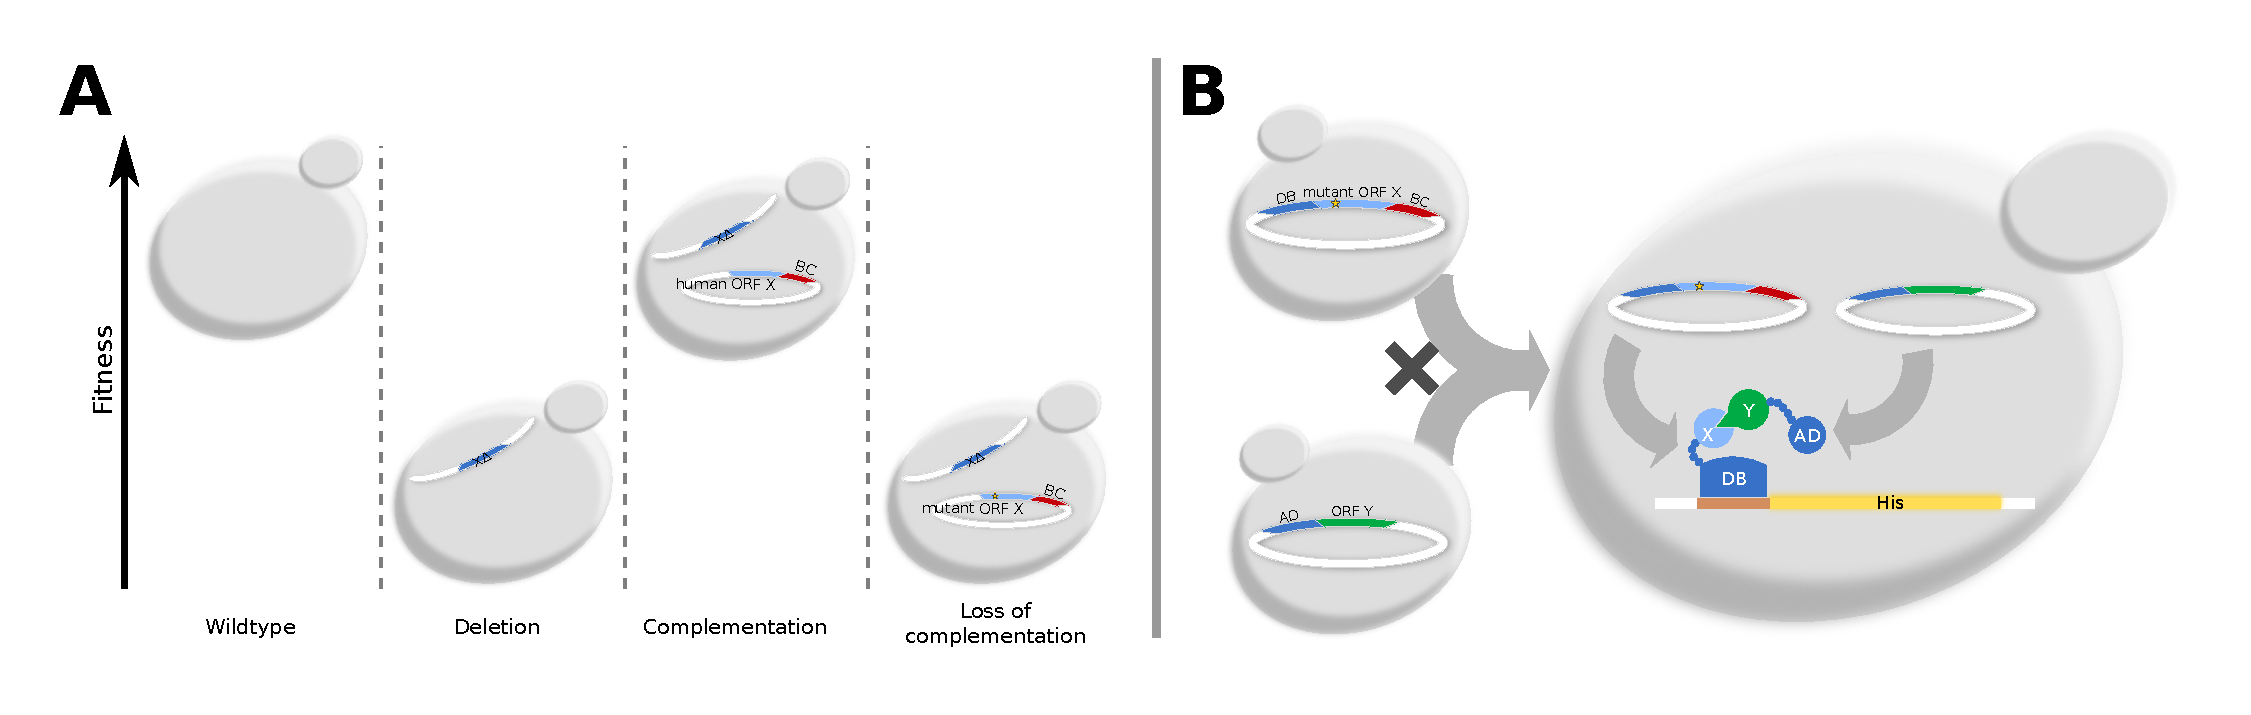
\includegraphics[width=\textwidth]{img/compl_y2h.pdf}
	\caption{Complementation and Yeast-2-Hybrid}
	\label{fig:compl_y2h}
\end{figure}
%Discuss Edgotyping?

Nonetheless, an assay that can measure the overall functionality of a protein within the cell would be preferable. Functional complementation~\cite{lee_complementation_1987} in yeast offers such an option. It based on the premise that some human genes can be used to rescue the deletion of their orthologues in yeast. That is, a fitness defect resulting from the inactivation of the yeast gene is alleviated by the artificial expression of the human gene. Therefore, any relative changes in fitness upon expressing a variant of the human gene can be interpreted as the variant's effect on the protein's overall ability to function. Song Sun and other members of the Roth Lab have recently examined the applicability of functional complementation in yeast to the assessment of disease variants~\cite{sun_extended_2016}. They have found an astonishing predictive capacity despite yeast and humans being diverged by a 1.5 billion year. Yeast complementation outperformed \textit{in silico} methods like PolyPhen-2 and PROVEAN in terms of disease variant prediction by a wide margin. At the 90\% specificity threshold discussed in section~\ref{insilicoIntro}, the complementation assay achieved a sensitivity of over 60\% (as compared to 19\% and 21\% for the two \textit{in silico} methods, respectively).

The only major drawback of yeast complementation is that currently only 60 human genes have been found to be amenable to the assay~\cite{sun_extended_2016}. %mention future outlook on human cell complementation and CRISPR? 

%Mention Phage display?


\section{Deep Mutational Scanning}

Complementation and Y2H promise to be useful tools in the classification of variants of uncertain significance. Yet applying them to retroactively test variants only once they have been found in the clinic would be a slow process. Instead, a proactive approach could prove to be more useful: Building an atlas of the functional effects of all possible variants before they are even seen in the clinic. This would require a massive parallelization of the assays. Indeed such parallelization efforts have previously been described, albeit not for the classification of VUS. Fowler and Fields have pioneered a technology called Deep Mutational Scanning (DMS)~\cite{fowler_high-resolution_2010}, which can be thought of as a natural extension to Alanine Scanning~\cite{cunningham_high-resolution_1989}, expanding it into the space of all possible amino acid changes. Fowler and Field's original paper has since inspired a fair number of similar efforts by other groups~\cite{ernst_coevolution_2010,fujino_robust_2012,adkar_protein_2012,mclaughlin_jr_spatial_2012,schlinkmann_critical_2012,whitehead_optimization_2012,traxlmayr_construction_2012,wu_systematic_2013,roscoe_analyses_2013,starita_activity-enhancing_2013,procko_computational_2013,tinberg_computational_2013,jiang_latent_2013,kim_high-throughput_2013,melamed_deep_2013,forsyth_deep_2013,wagenaar_resistance_2014,firnberg_comprehensive_2014,olson_comprehensive_2014,melnikov_comprehensive_2014,thyagarajan_inherent_2014,stiffler_evolvability_2015,doud_site-specific_2015,kitzman_massively_2015,starita_massively_2015,mishra_systematic_2016,doud_accurate_2016,mavor_determination_2016} (See Table~\ref{table:DMSstudies}). However, when considering these studies in the context of VUS classification, a number issues become apparent. Many of these have primarily used DMS in the context of biochemistry. The assays underlying different DMS studies are quite diverse and measure different aspects of a protein’s behaviour. As a consequence, they cannot be easily compared with each other. In addition, the achieved coverage of possible amino acid changes varies from map to map. Finally, many maps to do not control the quality of measurements. Therefore, the confidence levels underlying different parts of these maps are often unknown. A generalized framework that would allow for the construction of comparable, high-quality maps representing overall protein function would be of great utility.


\begin{landscape}
\begin{table}
	\centering
	\caption{Previous DMS studies}
	\label{table:DMSstudies}
	\begin{tabular}{l l l l l l l}
\textbf{Year} & \textbf{Authors} & \textbf{Protein} & \textbf{Region} & \textbf{Saturation} & \textbf{Selection} \\ \hline \hline
2010 & Fowler~\etal~\cite{fowler_high-resolution_2010} & YAP65 & WW domain & Very high & Phage display \\  
2010 & Ernst~\etal~\cite{ernst_coevolution_2010} & Synthetic protein & PDZ domain & ? & Phage display \\ 
2012 & Fujino~\etal~\cite{fujino_robust_2012} & Fab antibody fragment & fragment & Very high & Ribodisplay \\ 
2012 & Adkar~\etal~\cite{adkar_protein_2012} & Ccdb & whole protein & ? & Toxin activity in \species{E.~coli}\\ 
2012 & McLaughlin~\etal~\cite{mclaughlin_jr_spatial_2012} & PSD95 & PDZ domain & Very high & B2H+FACS (\species{E.~coli})\\ 
2012 & Schlinkmann~\etal~\cite{schlinkmann_critical_2012} & GPCR & whole protein & High & FACS (\species{E.~coli})\\ 
2012 & Whitehead~\etal~\cite{whitehead_optimization_2012} & Synthetic protein & whole protein & Very high & Yeast display \\ 
2012 & Traxlmayr~\etal~\cite{traxlmayr_construction_2012} & IgG1 & CH2/CH3 domains & ? & Yeast display \\ 
2013 & Wu~\etal~\cite{wu_systematic_2013} & Neuraminidase & SNP accessible & ? & Drug resistance (H1N1)\\ 
2013 & Roscoe~\etal~\cite{roscoe_analyses_2013} & Ubiquitin & whole protein & High & Yeast growth\\ 
2013 & Starita~\etal~\cite{starita_activity-enhancing_2013} & Ub.E3 E4B & whole protein & Low & Phage display\\ 
2013 & Procko~\etal~\cite{procko_computational_2013}  & Synthetic protein & 60AA & Very high & Yeast display\\ 
2013 & Tinberg~\etal~\cite{tinberg_computational_2013}  & Synthetic protein & 40AA & High & Yeast display\\ 
2013 & Jiang~\etal~\cite{jiang_latent_2013}  & Hsp90 & substrate binding loop & Very high & Yeast complementation\\ 
2013 & Kim~\etal~\cite{kim_high-throughput_2013}  & Mat alpha  & degron region & ? & Yeast growth\\ 
2013 & Melamed~\etal~\cite{melamed_deep_2013}  & Pab1 & RRM domain & High & Yeast complementation\\ 
2013 & Forsyth~\etal~\cite{forsyth_deep_2013}  & Antibody for EGFR & whole protein & Very high & Human cell display\\ 
2013 & Wagenaar~\etal~\cite{wagenaar_resistance_2014}  & BRAF & 77 Aas & ? & Drug resistance (Human)\\ 
2014 & Firnberg~\etal~\cite{firnberg_comprehensive_2014}  & TEM1-beta lactamase & Whole protein & High & Drug resistance (\species{E.~coli})\\ 
2014 & Olson~\etal~\cite{olson_comprehensive_2014}  & G protein (GB1) & IgG-binding domain & High & RNA display\\ 
2014 & Melnikov~\etal~\cite{melnikov_comprehensive_2014}  & APH(3′)II (kinase) & whole protein & Very high & Drug resistance (\species{E.~coli})\\ 
2014 & Thyagarajan~\etal~\cite{thyagarajan_inherent_2014}  & hemagglutinin & whole protein & ? & Viral replication (H1N1)\\ 
2015 & Stiffler~\etal~\cite{stiffler_evolvability_2015}  & TEM1 Beta-lactamase & whole protein & Very high & \species{E.~coli} growth\\ 
2015 & Doud~\etal~\cite{doud_site-specific_2015}  & influenza nucleoprotein & whole protein & ? & Viral replication (H1N1)\\ 
2015 & Kitzman~\etal~\cite{kitzman_massively_2015}  & Gal4 & DB domain & Very high & Yeast growth \\ 
2015 & Starita~\etal~\cite{starita_massively_2015}  & BRCA1 & RING domain & Low & Y2H + E3 activity\\ 
2016 & Mishra~\etal~\cite{mishra_systematic_2016}  & Hsp90 & ATPase domain & Very high & Yeast growth\\ 
2016 & Doud~\etal~\cite{doud_accurate_2016}  & Hemagglutinin & whole protein & ? & Viral replication (H1N1)\\ 
2016 & Mavor~\etal~\cite{mavor_determination_2016}  & Ubiquitin & whole protein & Very high & Yeast growth
\end{tabular}
\end{table}
\end{landscape}


Nonetheless, the existing studies allow for a survey of available methodologies and the structures they have in common. Deep Mutational Scanning can be broken down into a number of experimental and computational steps: (1) Mutagenesis; (2) Library construction; (3) Selection of functional mutants; (4) Sequencing of the pre- and post-selection libraries; and (5) Statistical analysis to determine the quantitative enrichment resulting from the selection. 

\begin{table}
	\centering
	\caption{Experimental steps in Deep Mutational Scanning}
	\label{table:DMSphases}
	\begin{tabular}{l p{10cm}}
	\textbf{Step}                & \textbf{Options} \\ \hline \hline
	Step 1: Mutagenesis          & Error-prone PCR, Kunkel, Oligo Array, Gene Synthesis\\ 
	Step 2: Library construction & Gibson Assembly, Gateway\\ 
	Step 3: Selection            & Complementation, Y2H, Phage display, Viral replication\\ 
	Step 4: Sequencing           & BarSEQ, Deep Sequencing\\ 
	Step 5: Analysis             & Enrich2\\ 
	\end{tabular}
\end{table}

The first step---mutagenesis---has been performed in different ways by different groups. The simplest method is error-prone PCR amplification~\cite{firstErrorPronePCR,mohan_pcr_2011}. While this has the advantage of being an inexpensive and facile procedure, it will only result in the generation of point mutations and as such will not generate all possible amino acid replacements. One may argue that the evaluation of VUS does not require insight into mutations outside of this set, however at the expense of potentially valuable biochemical insights. Another method often employed is Kunkel mutagenesis~\cite{kunkel_rapid_1985}. Originally developed as a method for simple site-directed mutagenesis, it can be scaled up to address a combination of multiple sites at once. It uses a special strain of \species{E.~coli} that has been modified to produce high levels of uradine and lacks the ability to excise uracil bases from DNA. A phage vector carrying the desired template sequence is transfected into the cells resulting in its replication with a high uracil incorporation rate. The thus uracilated template can be PCR amplified with primers containing the mutations of interest and subsequently amplified in regular \species{E.~coli} which will degrade the uracilated template, thus enriching the mutant copies. %More
A more recent development is the use of custom oligonucleotide arrays covering all possible (or desired) options of codon changes~\cite{kitzman_massively_2015}. These can then be used in linear amplification reactions with the gene template. While this option allows for the precise control of desired mutations, it is currently too expensive to be applicable at genome-scale. Similarly, mutagenesis libraries are becoming commercially available via gene synthesis~\cite{kosuri_scalable_2010}. While this method is certainly the most convenient, it is by far the most expensive option. A middle ground can be found in methods that employ amplification with oligonucleotides carrying degeneracy codons~\cite{pal_methods_2005}. Particularly popular is the use of NNK and NNS degeneracies, which have long been used in biochemistry~\cite{scott_searching_1990,barbas_semisynthetic_1992}. Here, S denotes Guanine or Cytosine and K denotes Guanine or Thymine in the third position of the codon. While either of these codes only allow 32 of all 64 possible codons to be formed, they do cover all 20 possible amino acids, while avoiding two of the three possible stop codons (opal and ochre).

Library construction is the second step in any DMS experiment. The choice of method in this step is dependent on the type of selection and sequencing used in the later steps. Some methods require mutants to be tagged with molecular barcodes, i.e. short unique DNA sequences inserted at a known location that allow identification of a molecule with just a single sequencing read. While the use of barcodes greatly simplifies the readout of the selection result it does require that the contents of the library are catalogued at the time of construction.

Step three of a DMS procedure is the selection of mutants that pass a given assay. In most cases, assays are designed to test for protein protein interactions, for example via Y2H or phage display~\todo{REF}. In other cases it may be overall protein function, as measured by complementation or in cases of viral proteins, the ability of the virus to replicate.

The fourth step in the procedure is sequencing. 

%The original method used phage display as a method of selection on an exhaustive library of mutant proteins followed by deep sequencing to identify which mutant proteins were enriched in the process. While the original method was developed as an extension to alanine scanning~\cite{alanineScanning} in the pursuit of biochemical insights, it can certainly be adapted to work with other selection methods such as Y2H and complementation. Indeed, \todo{Who?} and colleagues have recently adapted it to the use of complementation as a means of selection.
% \section{Edgotyping}

\section{Background: The Sumoylation Pathway}
\label{intro:sumoylation}

In the following chapters, we will evaluate the performance of sequence-function technology such as Deep Mutational Scanning with respect to its ability to detect effects not only on overall function but individual subfunction. Beyond the amenability of the proteins to the employed assays, an ideal testing ground would be comprised of a biological system that is both mechanistically complex and has been well studied previously in terms of structure and mechanism. The Sumoylation life cycle does not only fulfill these criteria, but is also of great biological importance. Sumoylation is a protein modification in which a small ubiquitin-like modifier (SUMO) is covalently attached to target proteins in order to modulate their behavior, especially in terms of localization and physical interactions~\cite{sumoylation}. Sumoylation plays an important role in a large number of cellular processes. It is therefore not surprising that the core members of the pathway are essential genes~\todo{REF}.

\begin{figure}
	\centering
	\includegraphics[width=\textwidth]{img/sumoylation_steps.pdf}
	\caption{Steps in the sumoylation cascade. SENP protease matures a SUMO precursor by cleaving off its four C-terminal residues. In the activation step, the E1 complex forms a thioester bond  between SUMO and one of its cysteine residues under ATP consumption. It then transestereficates SUMO to the E2. The E2 recognizes potential targets via their $\Psi$KXE motif. With the help of an E3, SUMO is then ligated to the central lysine within that motif. SENP proteases can reverse the process by hydrolysing this new peptide bond. Images are based on the following PDB structures: \texttt{2G4D}~\cite{Xu2006}, \texttt{3KYC}~\cite{Olsen2010}, \texttt{4W5V}~\cite{ReiterEtAl}, \texttt{3UIP}~\cite{Gareau2012}}
	\label{fig:sumoylation_steps}
\end{figure}

Despite employing a distinct set of proteins compared to the ubiquitination machinery, the sumoylation pathway bears many close similarities. Analogously to ubiquitin, an enzymatic cascade of proteases, E1, E2 and E3s guide SUMO through its maturation, activation, conjugation and ligation phase~\cite{sumoylation} (Figure \ref{fig:sumoylation_steps}). After expression, SUMO is matured through cleavage of four amino acids from its C-terminus, exposing a diglycine motif. In humans, this process is performed by two proteases, SENP1 and SENP2. Next, an E1 activation complex (UBA2-SAE1) forms a thioester bond between the SUMO C-terminal diglycine and a cysteine residue within the E1 protein under the consumption of ATP. An E2 conjugase (UBE2I) binds to the complex, so that the activated SUMO can be transfered to one of its own cysteine residues via transesterification. 

The thus loaded E2 can recognize potential target proteins via an exposed motif of four amino acids. The motif is generally described as $\Psi$KxD/E, i.e. a large hydrophobic residue, followed by a lysine, a spacer residue and an acidic residue~\cite{Sampson2001}. The motif is often found in an extended loop extending from the protein or in a disordered region~\todo{REF}. The central lysine within the motif enters the E2’s active site where it comes into contact with the SUMO diglycine. There, a peptide bond is formed between the lysine $\varepsilon$-amino group and the SUMO C-terminus~\cite{BernierVillamor2002}. This process can be made more efficient in the presence E3 proteins. It is interesting to note, that while only a single SUMO E2 conjugase (UBE2I) is encoded by the human genome, there is a variety of different SUMO E3 ligases. Some work by simply stabilizing the SUMO-E2 complex, while others can outright force-feed non-canonical targets to the E2~\cite{Streich2016}. 

\begin{figure}[h!]
	\centering
	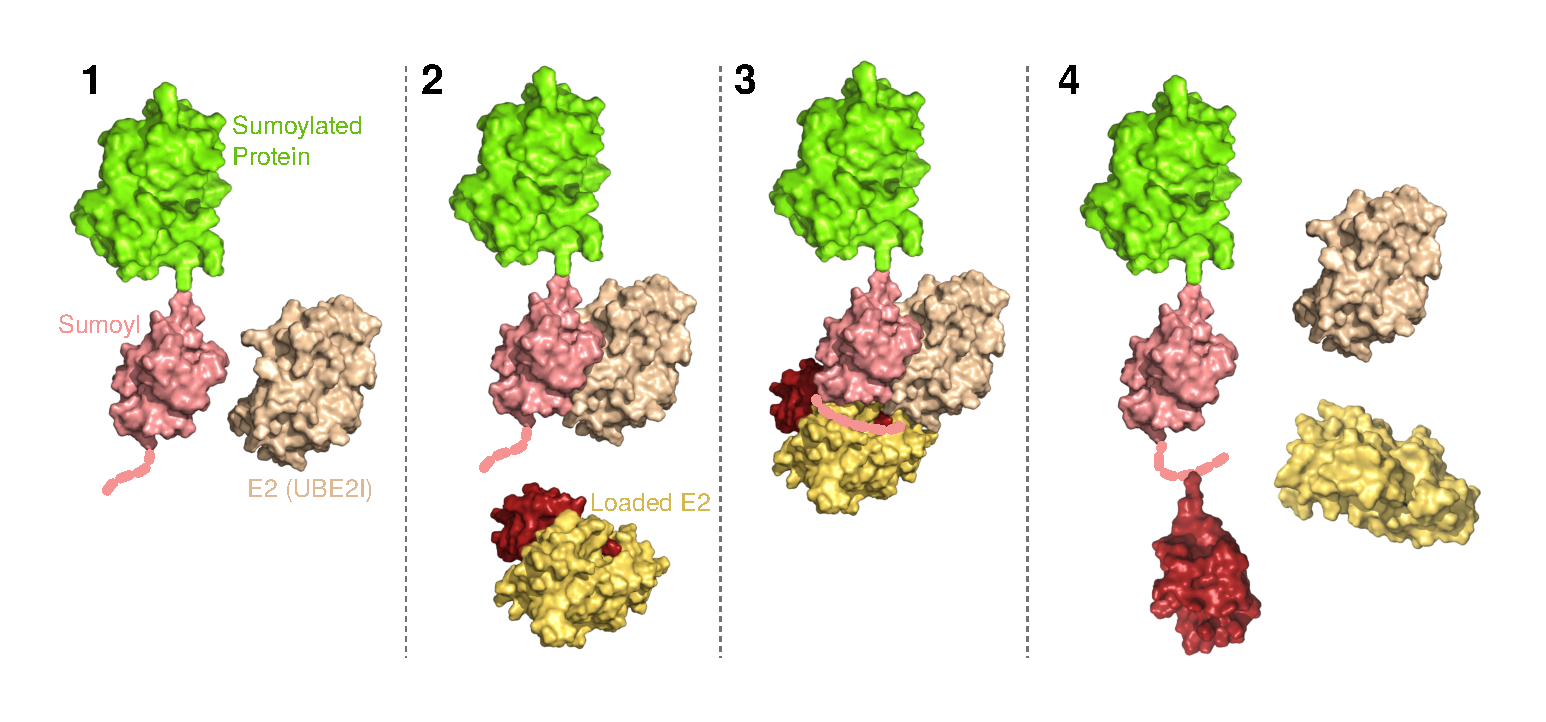
\includegraphics[width=\textwidth]{img/sumo_chaining.pdf}
	\caption{Steps in SUMO chain formation as proposed by Alontaga and colleagues~\cite{Alontaga2015}. An E2 noncovalently interacts with a SUMO modification of a target protein. A second E2 carrying a covalently bound second SUMO binds the first E2-SUMO complex, allowing for the first SUMO's N-terminal tail to enter the active site, where a lysine within the tail is forms a peptide bond with the second SUMO's C-terminus. Finally, the complex dissociates, leaving behind the newly formed SUMO chain. Images are based on the following PDB structures: \texttt{3UIP}~\cite{Gareau2012}, \texttt{4Y1L}~\cite{Alontaga2015}}
	\label{fig:sumo_chaining}
\end{figure}

Like ubiquitin, SUMO can also form chains (Figure \ref{fig:sumo_chaining}). However, of the four SUMO proteins encoded by the human genome, only SUMO2 and SUMO3 are capable of doing so, as they contain a suitable lysine residue within a disordered N-terminal tail\todo{REF}. Capili and Lima previously observed that the E2 (UBE2I) and SUMO can interact in a noncovalent manner via a distinct binding interface~\cite{CapiliLima2007}. According to a model proposed by Alontaga and colleagues~\cite{Alontaga2015} this interaction is a key mechanism in SUMO chain formation. The interaction recruits a second, SUMO-loaded E2 that interacts with the complex in such a manner that the lysine within the first SUMO's N-terminal tail can find its way into the active site of the second E2, where the second SUMO is concatenated.



Given the complexity of the Sumoylation system, especially surrounding the E2 component, an examination of sequence-structure-function relationships becomes a multifaceted problem. Mutations could in principle affect any combination of the multiple interaction interfaces which in turn contribute in complex ways to the overall cellular phenotype.
An alanine scan of the yeast SUMO E2 Ubc9 was previously performed and succeeded in identifying functionally important sites within the protein 20. Similarly, a DMS scan of ubiquitin, was previously completed 21. While both of these projects provided great insight into the biochemistry of ubiquitin-like protein pathways, neither has produced a complete map.
%Sampson2001: The small ubiquitin-like modifier-1 (SUMO-1) consensus sequence mediates Ubc9 binding and is essential for SUMO-1 modification. 
%BernierVillamor2002: Structural basis for E2-mediated SUMO conjugation revealed by a complex between ubiquitin-conjugating enzyme Ubc9 and RanGAP1.
%Streich2016: Capturing a substrate in an activated RING E3/E2–SUMO complex
%CapiliLima2007: Structure and analysis of a complex between SUMO and Ubc9 illustrates features of a conserved E2-Ubl interaction
%Alontaga2015: RWD Domain as an E2 (Ubc9)-Interaction Module
%Xu2006: http://www.biochemj.org/content/398/3/345
%Olsen et al. 2010 (Lima Lab) Active site remodelling accompanies thioster bond formation in the SUMO E1
%Katherine H. Reiter‡, Anita Ramachandran‡, Xue Xia‡, Lauren E. Boucher‡,§, Jürgen Bosch‡,§ and Michael J. Matunis‡1Characterization and Structural Insights into Selective E1-E2 Interactions in the Human and Plasmodium falciparum SUMO Conjugation Systems.




\chapter[A comprehensive high-fidelity DMS framework]{A framework for comprehensive and high-fidelity Deep Mutational Scanning}
\label{ch:data1}

\section{Introduction}

% \todo{Cast this introduction more in the light of functional assays and less about disease. (Save that for the next chapter.)}

Deep Mutational Scanning~(DMS)~\cite{fowler_high-resolution_2010}, a strategy for large-scale functional testing of variants, is yielding functional maps describing a large fraction of substitutions for an often substantial subset of residue positions. The assays used for DMS studies are diverse, often measuring different aspects of a protein's behaviour. Functional complementation assays test a variant's impact on overall protein function by testing the variant gene's ability to rescue the phenotype caused by reduced activity of the wild type gene (or its ortholog in the case of trans-species complementation)~\cite{lee_complementation_1987,osborn_rescuing_2007}. In a previous paper, Song Sun and other members of the Roth Lab have previously found cell-based functional complementation assays to accurately identify disease variants across a diverse collection of human disease genes~\cite{sun_extended_2016}. 

There are many challenges to the DMS strategy.  One challenge is establishment of robust interpretable assays that measure each variant's impact on the disease-relevant functions of a gene. Another is that the fraction of possible amino acid changes that are measured varies from map to map. Finally, many maps do not control the overall quality of measurements, or estimate the quality of each measurement. The lack of a comprehensively measured map of known-quality functional impact scores limits the opportunity for confident use of DMS maps to evaluate specific variants.

Here we describe a modular DMS framework to generate  complete, high-fidelity maps of variant function based on functional complementation. The framework employs a novel mutagenesis strategy, two alternative sequencing-based selection screens, and a machine learning strategy to impute  otherwise missing parts of the map with surprising accuracy, and uses regularization to correct less confidently measured data points. We evaluate our framework on the SUMO E2 conjugase UBE2I.


\section{Results}

To carry out deep mutational scans of protein sequences yielding comprehensive atlases of sequence-function relationships, we found it useful to organize the process into six stages (see Figure~\ref{fig:framework}): 1) mutagenesis; 2) generation of a clone library; 3) selection for clones encoding a functional protein; 4) read-out of the selection results and analysis to produce an initial sequence-function map; 5) computational analysis to impute missing values; and 6) computational analysis to refine measured values based on imputation models. This framework incorporates previously-described deep mutational scanning concepts as well as new experimental components (e.g., our saturation codon mutagenesis strategy) and analytic methods.  The last two stages enabling a complete and accurate DMS map have not been applied in any published DMS study.

We first describe a variant of the framework called DMS-BarSeq and apply it to the human SUMO conjugase UBE2I, exhaustively measuring the ability of protein variants to function and to physically interact with protein partners.  Next, we describe a more efficient DMS-TileSeq variant of the framework, and apply this to UBE2I.  Having combined these maps, we computationally infer missing data points and refine map quality.


\begin{figure}[h!]
	\centering
	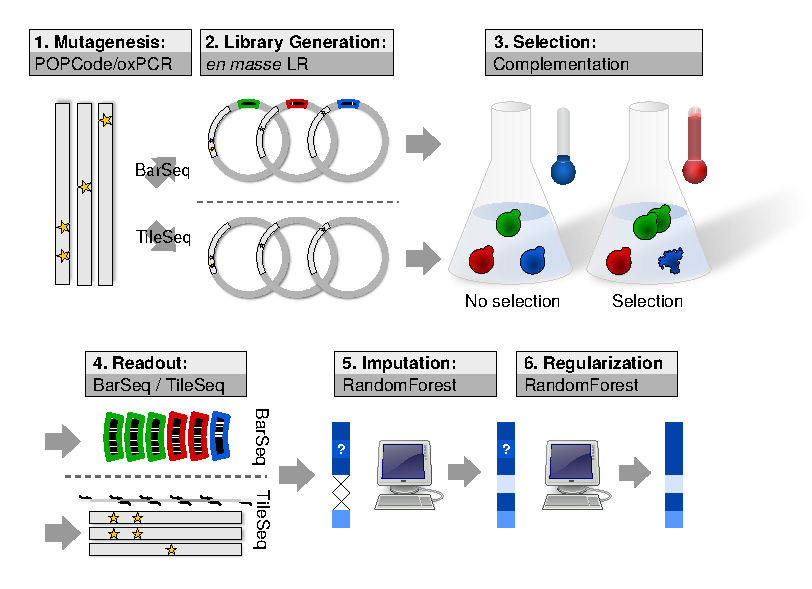
\includegraphics[width=\textwidth]{img/framework_flowchart.pdf}
	\caption{An overview of the Deep Mutational Scanning Framework. Step 1: Using mutagenesis via POPCode and oxidized nucleotide PCR, a pool of variant ORFs is created. Step 2: A library is generated via en-masse gateway cloning. Depending on the downstream sequencing procedure either plain or barcoded expression vectors are used. Step 3: Clones compete with each other for growth under selective and control conditions. 4: In case of BarSeq, barcodes are sequenced and counted. In case of TileSeq, individual tiles within the ORF are amplified used in paired-end sequencing. Step 5: Machine Learning methods are used to impute the effects of missing variants. Step 6: Machine learning predictions are also used to support less confidently measured variants. }
	\label{fig:framework}
\end{figure}


\subsection{A barcode-based Deep Mutational Scanning strategy}

%Describe goals for this screen, and then how the different choices below aim to achieve these.

As an initial test of the overall framework, we first aimed to generate a map of functional missense variation for UBE2I. Our goals for this map were as follows: (i) High and even coverage of the full spectrum of amino acid changes;(ii) Determination of mutant effects on overall protein functionality; (iii) High fidelity of functional effect readouts. We therefore designed the different stages of the framework accordingly. 

For Stage 1 of the DMS framework---mutagenesis--- to achieve a relatively even representation of all possible single amino acid substitutions, we wished to allow multiple mutations per clone. This would not only allow for greater mutational coverage for any given library size, but it would also offer an opportunity to discover intragenic epistatic relationships between variants.  To fulfill these requirements, we developed a mutagenesis protocol (Precision Oligo-Pool based Code Alteration or POPCode) which generates random codon replacements. 
At the second stage---library generation---we wished to be able to track the fitness effects of each individual mutant clone rather than just average effects of mutations across the population, as this could be expected to allow for higher quality measurements. Thus, in Stage 2 of the framework, we opted to assign molecular barcodes to each clone that could be identified by sequencing. To catalogue the pairing of mutant genotypes with barcodes, we developed a novel multiplex amplicon sequencing method called KiloSeq, in collaboration with SeqWell Inc, Boston. 
The selection process (Stage 3) was performed as a yeast complementation assay, to allow for determination of overall functional effects of mutations. The assay would be performed as a time series in triplicates, as this again promised to allow for higher quality of readouts 
Finally, Stage 4, would consiste of barcode sequencing and statistical analysis. All four stages will be described in further detail in the following subsections.


\subsubsection{POPCode: A Precision Oligo Pool Codon alteration mutagenesis method}

This method scales up a previously described method developed by Seyfang~\etal~\cite{seyfang_multiple_2004}. To achieve complete wide coverage over the complete spectrum of possible amino acid changes we design oligonucleotides centering on each codon in the Open Reading Frame (ORF) of interest and replacing the target with an \texttt{NNK} degeneracy code. As explained in chapter~\ref{intro:mutagenesis}, this has been previously used to allow all amino acid changes while reducing the chance of generating stop codons~\cite{pal_methods_2005}. 
In the next step, the ORF sequence is PCR amplified in the presence of dUTP to generate uracil-doped template for the mutagenesis reaction. Oligonucleotide pools were then hybridized with the template. Gaps between hybridizations were filled with non-strand-displacing polymerase. 

When finding a set of suitable oligonucleotide sequences, two important criteria need to be considered: 
(i) The melting temperature across the complete set is as uniform as possible as this will ensure a more even mutation rate across the ORF sequence; (ii) the degenerate codon sequence should be located as close to the center of the oligo as permissible given the first criterium. To simplify the process of choosing an appropriate set of oligos based on these criteria I developed a web tool that can be used to calculate the optimal solution to the given problem. The tool merely requires the sequence of the target ORF and flanking vector sequences, a desired average oligo length and a maximum offset parameter. The offset parameter determines how many bases can be maximally added or removed from each side of a given oligo to optimize its melting temperature. 

In some cases a moderate deviation from the average in melting temperature for some oligos cannot be avoided. To alleviate these effects, the webtool also offers a mutation rate prediction. This is based on observations from all the POPCode procedures performed as part of this work in combination with linear regression. The prediction can be used to preemptivly adjust concentrations of potentially troublesome oligos in the POPCode protocol. An additional webtool feature based on the mutation rate prediction is the automatic calculation of necessary library size to achieve a desired mutational coverage. The webtool as available at \verb|http://llama.mshri.on.ca/cgi/popcodeSuite/main|.

%%Figure: PopCode schema

\begin{figure}[h!]
	\centering
	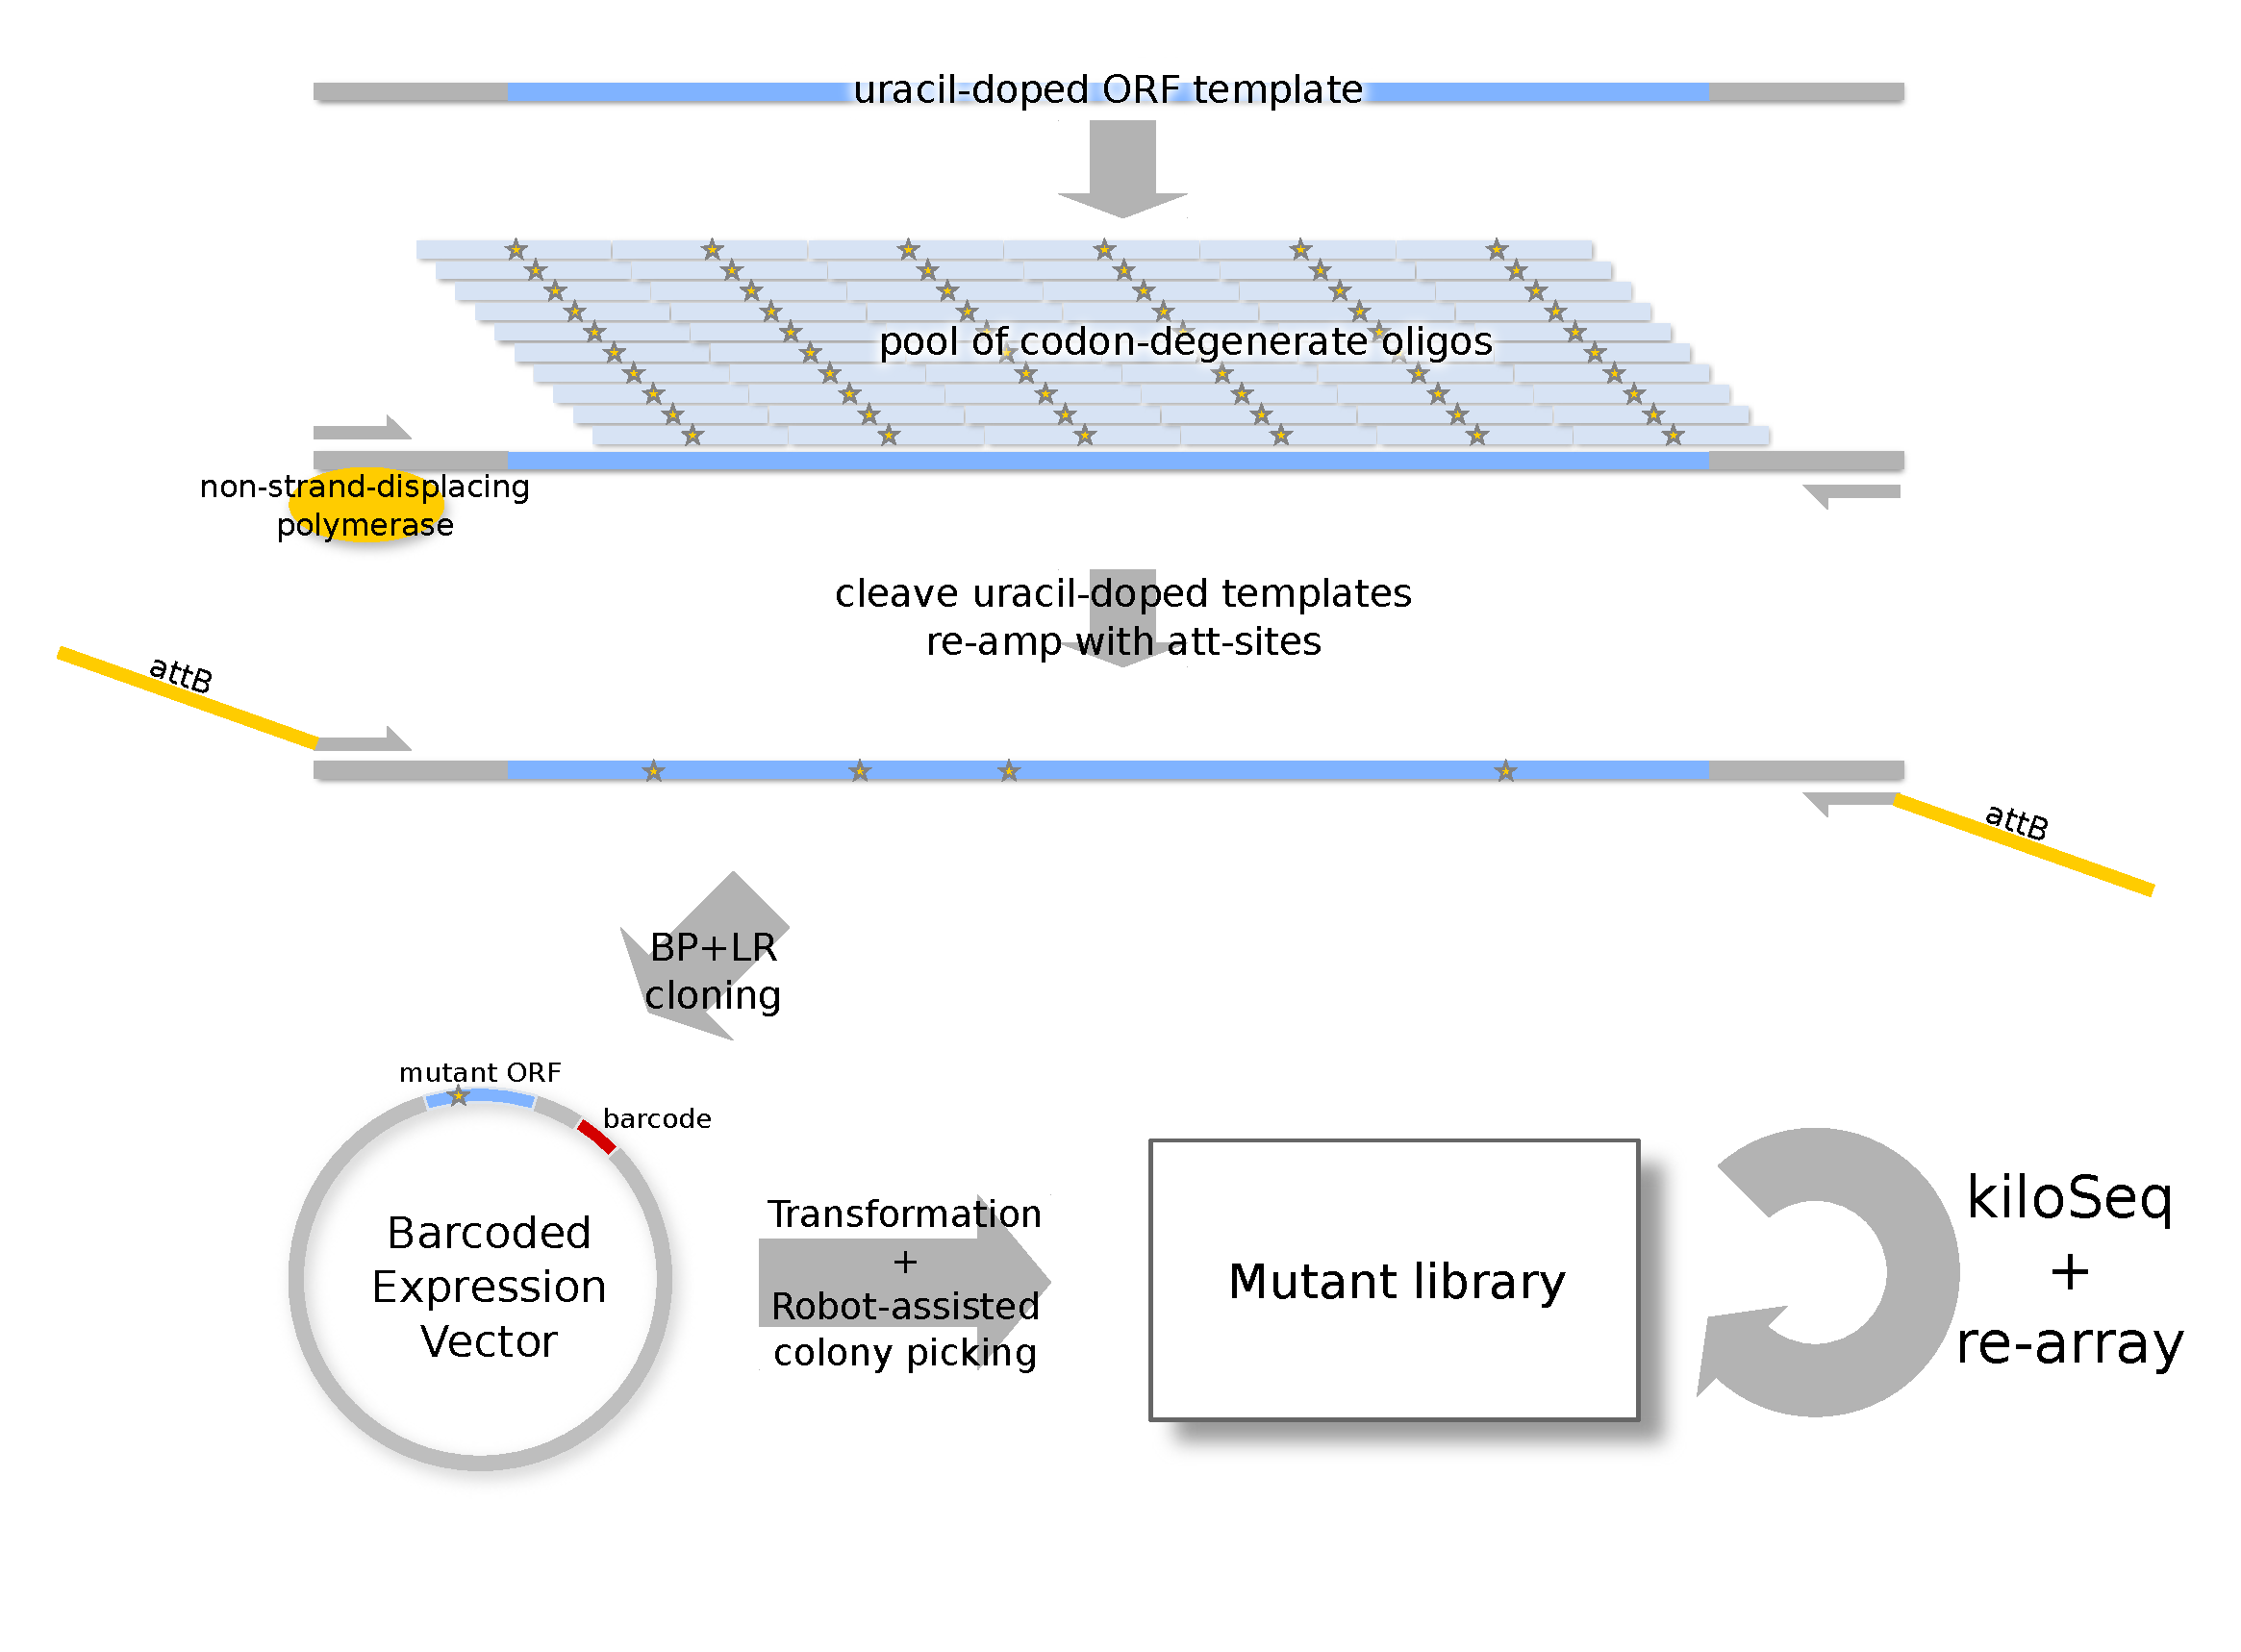
\includegraphics[width=\textwidth]{img/popcode_schema.pdf}%TODO: should be direct BP-LR cloning
	\caption{POPCode mutagenesis and library generation. A pool of codon-denerate oligos is hybridized to a uracil-doped template, gaps between oligos are closed via non-strand-displacing polymerase and the backbone sealed. Uracil-doped template is degraded to enrich for mutants. After mutagenesis, Gateway attB sites are added, followed by BP+LR cloning into barcoded vectors and transformation into bacteria. Finally, colonies are picked and arrayed.}
	\label{fig:popcode_schema}
\end{figure}
Following cleanup, the uracil-doped template was incapacitated using Uracil-DNA-Glycosylase (UDG). The mutagenesis product was then amplified with primers that added attB sites to allow Gateway BP cloning into entry vectors.

To accomplish mutagenesis across the entire coding region of our gene of interest, \gene{UBE2I}, we designed a tiled collection of oligos (one per codon) and applied POPCode to generate a codon-mutagenized amplicon library.  In parallel, we carried out PCR with oxidized nucleotides~\cite{mohan_pcr_2011} to enable deeper representation of amino acid changes achievable from single-nucleotide changes.

\subsubsection{Library generation and highly multiplexed amiplicon sequencing}

For Stage 2 of the framework---generation of a clone library---we employed an \textit{en masse} recombinational cloning strategy to generate a Gateway Entry vector library of \gene{UBE2I} variants. This library was transferred via \textit{en~masse} recombinational subcloning into a pool of randomly-barcoded plasmids enabling expression of \gene{UBE2I} variants in yeast. As sequencing is required to establish the full-length ORF sequence and barcode of each clone, the complementation vector is designed such that the variant ORF and the barcode locus are in close proximity to each other. Thus, only a relatively small segment of the plasmid needs to be inspected to determine the pairing of genotype and barcode. 

After bacterial transformation, we proceeded to robotically pick 19,968 colonies, which were stored in 52 384-well plates. As sequencing needs to be performed to catalogue the identities of nearly 20,000 individual samples, we used a novel sequencing method called KiloSeq which combines plate-position-specific index sequences with Illumina sequencing (Figure~\ref{fig:kiloseq_schema}).
KiloSeq was developed in collaboration with SeqWell Inc., Boston. First, for each clone in the library, the region of interest is amplified with primers containing well-specific tags, uniquely identifying each well coordinate. This step is dependent on the use of a HydroCycler, which allows up to 4608 PCR reactions to be performed in parallel. In the next step, wells for each plate can be pooled. Nextera tagmentation using Tn5 transposase is used to break the amplicons into random fragments and simultaneously ligate them to Illumina sequencing linkers with plate-specific indices. We then re-amplify the pool with  3'-specific primers, to enrich for fragments that contain the well tags. The resulting library is now ready for paired-end sequencing. In each pair of reads, one read will contain the well tag and the barcode locus, whereas the other will contain a fragment of the mutant ORF.
%TODO: move to methods: This is done using a hydrocycler, allowing for thousands of PCR reactions to be performed in parallel. ----- Amplicons can then be plate-wise pooled.

\begin{figure}[h!]
	\centering
	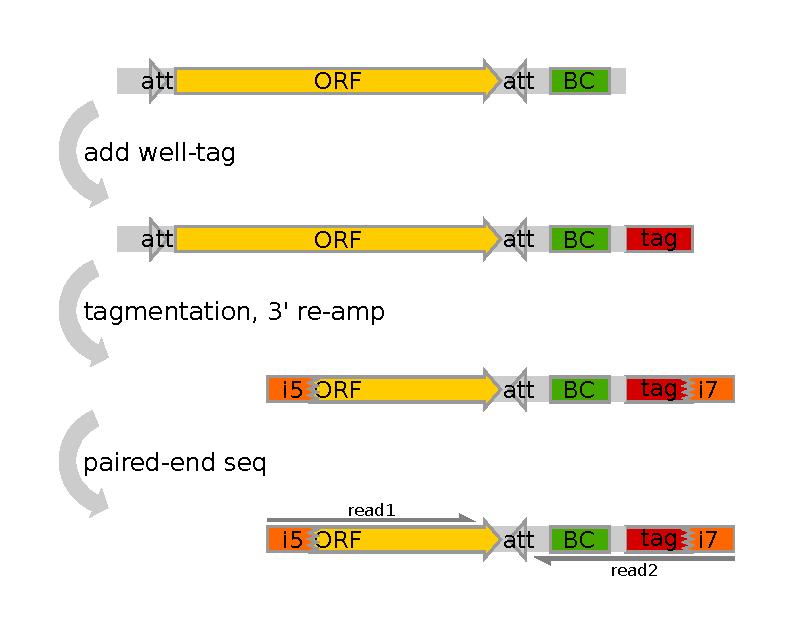
\includegraphics[width=.5\textwidth]{img/kiloseq_schema_new.pdf}
	\caption{KiloSeq schema. 1) For each library well, amplicons containing the variant ORF (gold) and Barcode locus (green) are amplified with primers adding a well-specific tag. 2) Tn5 tagmentation fragments the DNA while simultaneously adding Illumina i5/i7 linkers. 3' re-amplification enriches for fragments containing the well tags. 3) Each pair of sequencing reads now contains a fragment of ORF sequence and the associated barcode and well tag.}
	\label{fig:kiloseq_schema}
\end{figure}

To process the results of a KiloSeq sequencing run, a special software pipeline was developed, which can be divided into three phases: demultiplexing; barcode clustering; and alignment and variant calling.
The first phase---demultiplexing---takes place on two levels, corresponding to library plates and the wells within those plates. Demultiplexing at plate level is performed by Illumina's bcl2fastq software, which resolves i5-i7 index combinations. The second phase is performed on a high performance computing cluster. Sets of read pairs are distributed across computing nodes, where they are processed by worker scripts. The well-tag within each R2 read is identified using a k-mer search algorithm, and read-pairs are sorted accordingly into bins. Each bin corresponds to one well in a given plate. At the same time, barcode sequences are extracted from the R2 reads in preparation for the next phase. 

The second phase---barcode clustering---uses the extracted barcode sequences within each bin and clusters them according to their Levenstein distance~\cite{levenshtein_binary_1966} (i.e. the number of edit operations required to transform one into the other). This step is necessary in order to resolve possible contamination across wells that occurred during library preparation. Each barcode cluster corresponds to a different clone, and the different unique sequences within each clusters correspond to different sequencing errors. The most frequently observed sequence within each cluster is interpreted as the true barcode. Finally, read pairs within each bin are again subdivided according to their respective barcode cluster.

The third phase---alignment and variant calling---is then executed for each barcode cluster within each well within each plate. The R1 reads are aligned to the template sequence and variants are called. This is complicated by the fact that the KiloSeq library preparation usually creates a certain amount of cross-contamination between wells. While single or multi-nucleotide variants are still relatively unproblematic to identify, standard tools were found to be unable to identify copy number variations (CNVs) due to these problems. We thus developed a custom method for CNV calling, based on detecting sudden changes in read depth across the alignments. First the individual read depth track is normalized to the average read depth across the plate. Then a one-dimensional Sobel operator is used to detect sharp edges in the signal. An example of this can be seen in Figure~\ref{fig:border_detect}. Detection thresholds were optimized by comparison with Sanger sequencing.

\begin{figure}[h!]
	\centering
	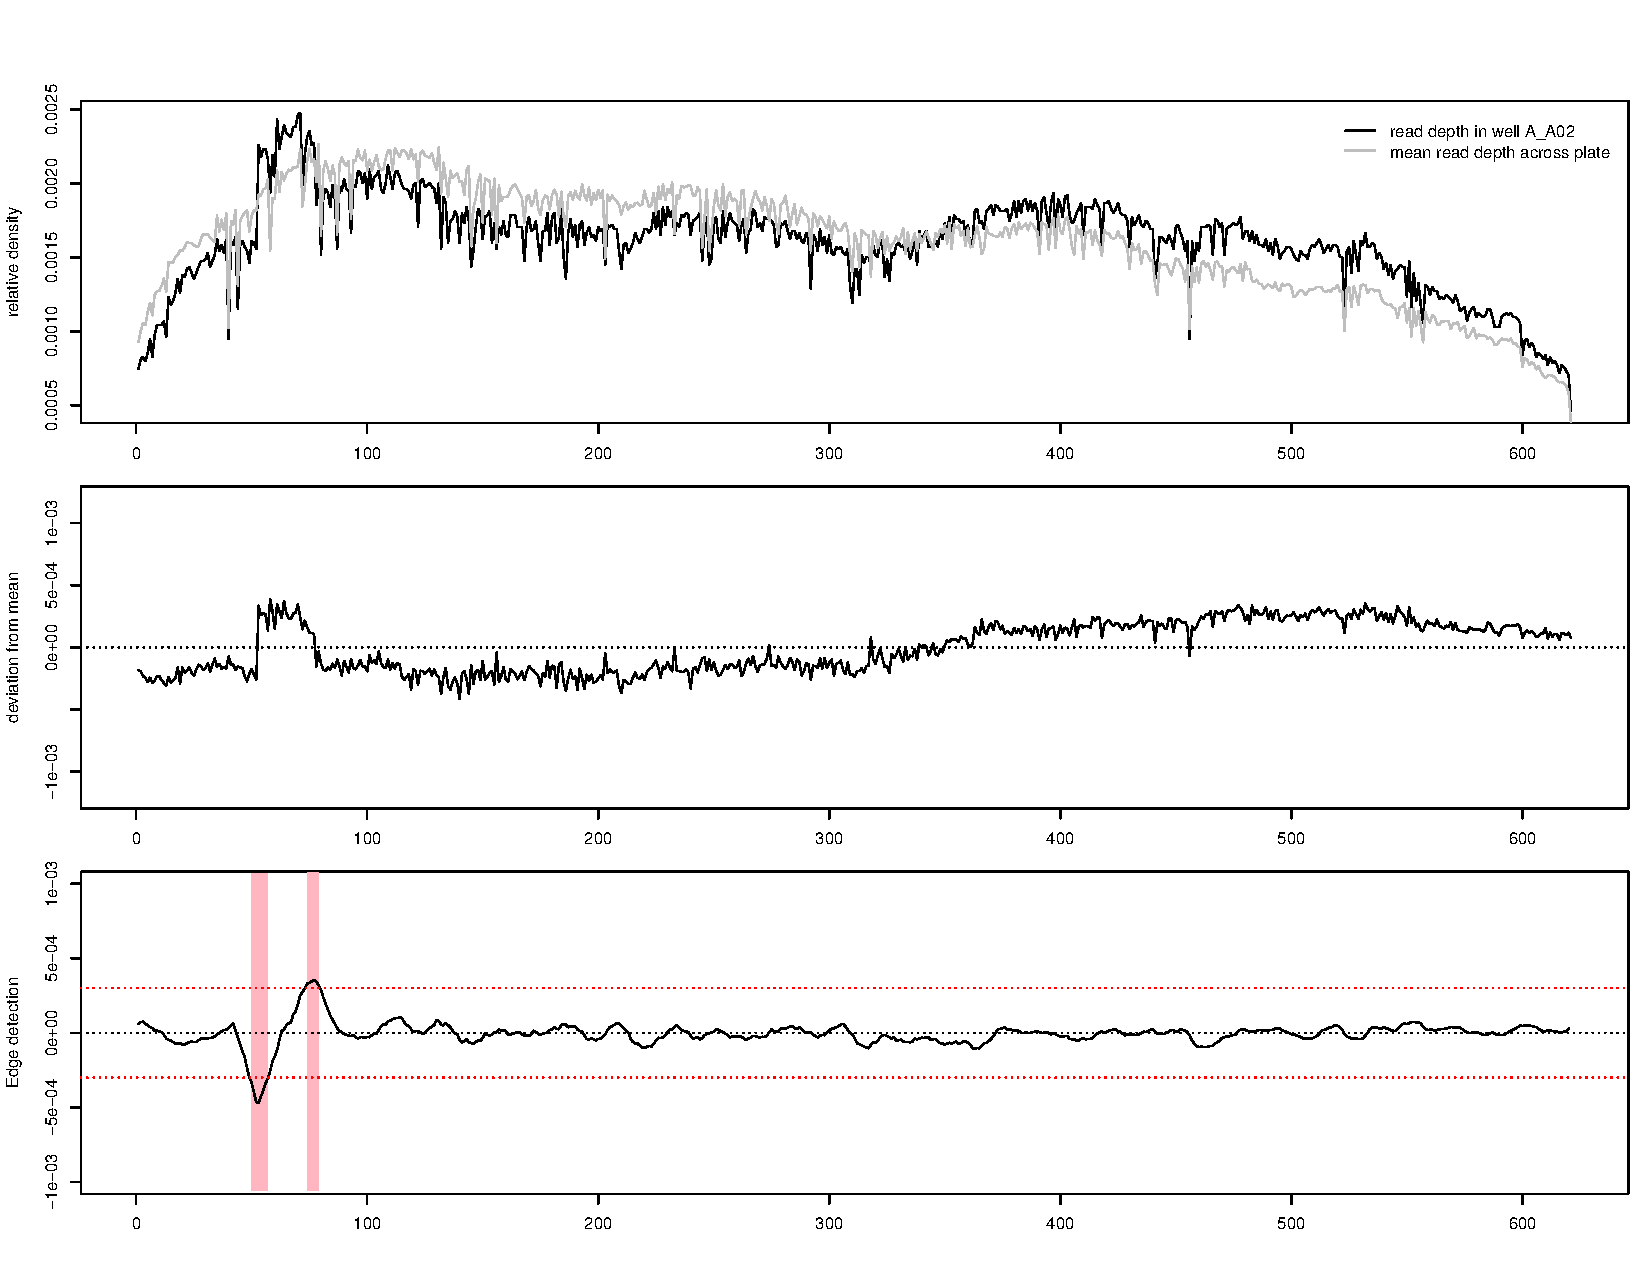
\includegraphics[width=\textwidth]{img/border_detect.pdf}
	\caption{Indel detection example. A duplication event in well \texttt{A\_A02} is detected by normalizing relative read depth by the mean depth across the plate and using a Sobel operator to detect sudden changes.}
	\label{fig:border_detect}
\end{figure}


After successful genotyping with kiloseq, we determined the subset of clones that (i) contained at least one missense mutation, (ii) did not contain any insertions or deletions, (iii) did not contain mutations outside of the ORF, (iii) had unique barcodes, (iv) had sufficient read coverage during KiloSeq to allow for confident genotyping.
Over half of clones in the library conformed to these criteria. The single largest reason for exclusion was the occurrence of indels and CNVs (Figure~\ref{fig:popcode_census}A). 

An analysis of the mutation signatures across clones generated by POPCode revealed that two different mechanisms appear to underly mutagenesis. When considering only mutations that change more than one base in a given codon, there is an equal chance for every possible base except in the third position, where almost no adenine or cytosine was introduced. This is consistent with the NNK degeneracy code used in the POPCode oligo design. By contrast, variants that change only a single base in a given codon show a strong bias for transitions over transversions. These could be introduced due to polymerase error (Figure~\ref{fig:popcode_census}B). This is also reflected in the relative share of single nucleotide variants, which make up 56\% of mutations (Figure~\ref{fig:popcode_census}C). As a consequence, when examining the mutation coverage across the sequence of the ORF, it is clearly visible that the share of amino acids reachable with a single nucleotide change from the respective wildtype codon is much closer to saturation than the the set of all possible amino acid changes (Figure~\ref{fig:popcode_census}D). Additionally some hotspots are visible, in which mutation rate is higher, which is likely due to different hybridization efficiencies of oligos across the ORF sequence.

Using the Biomatrix robot, we re-arrayed the subset of usable clones into a condensed final library of 40 plates. This final library comprised 6,553 \gene{UBE2I} variants, covering different combinations of 1,848 (61\% of all possible) unique amino acid changes. In preparation for the next stage, variant plasmids were pooled, together with barcoded empty vector and wild type control plasmids.

\begin{landscape}
\begin{figure}[h]
	\centering
	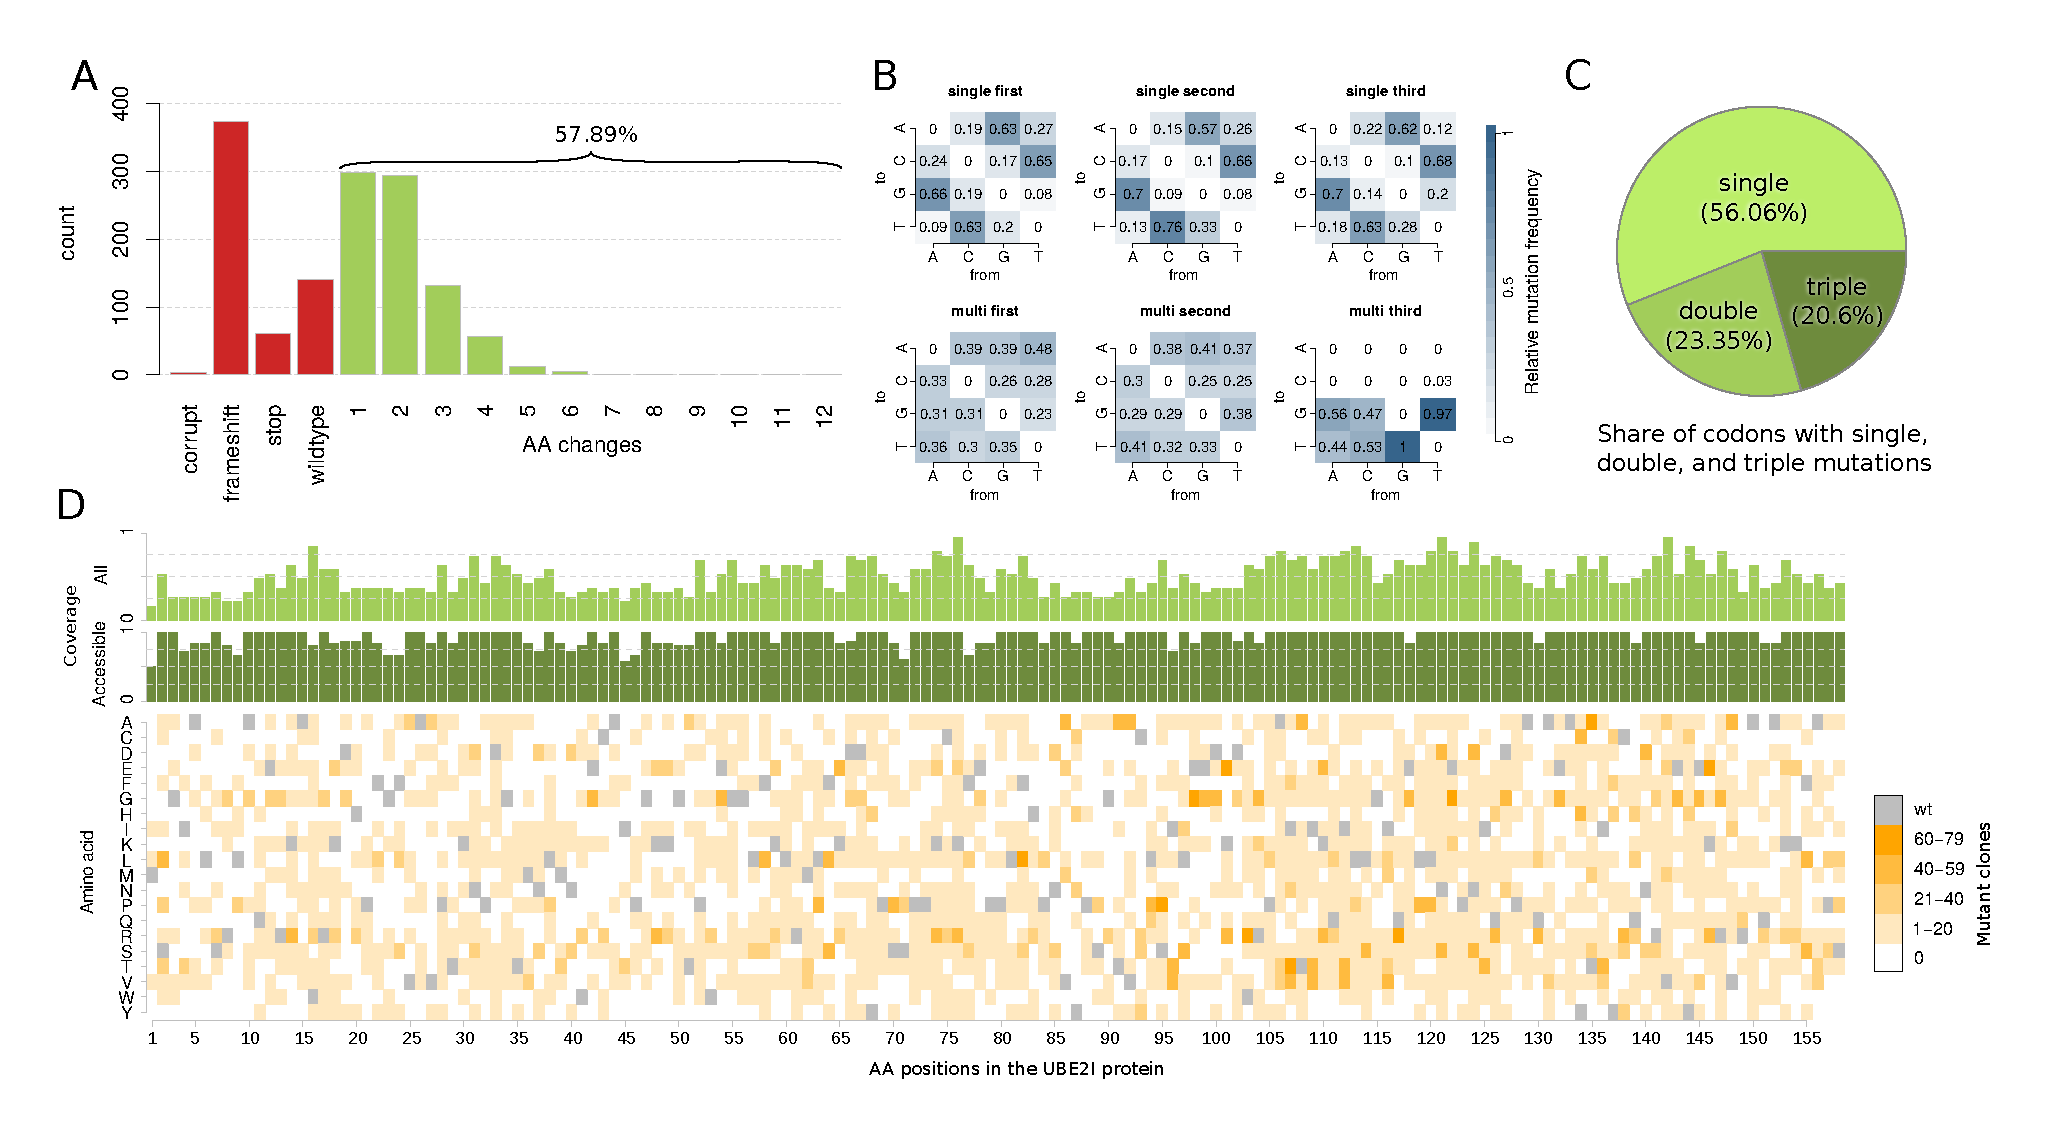
\includegraphics[width=9in]{img/popcode_census.pdf}
	\caption{KiloSeq census of \gene{UBE2I} POPCode library. A) Breakdown of KiloSeq results for a set of five 384 well plates of mutant clones generated by POPCode. Corrupt: Clones containing mutations outside of the ORF; Frameshift: Clones containing indels or copy number variants; Stop: Clones containing stop codons. B) Breakdown of mutations in codons. Top: Single nucleotide variants; Bottom: Multi-nucleotide variants. Columns correspond to the first, second and third position in a codon. C) Relative shares of single, double and triple nucleotide variants among all missense variants in the library. D) Coverage map of missense variants in the library. Light green track: Coverage across all possible amino acids; Dark green track: Coverage across amino acids reachable with a single nucleotide change from the wildtype codon.}
	\label{fig:popcode_census}
\end{figure}
\end{landscape}



\subsubsection{Complementation screen and Barcode sequencing}

For Stage 3---the selection of clones encoding a functional protein---we employed a previously described \species{S.~cerevisiae} functional complementation assay~\cite{lee_complementation_1987,osborn_rescuing_2007}. This assay is based a yeast strain carrying a temperature sensitive (ts) allele of the \gene{UBE2I} orthologue \gene{UBC9}. Expression of human \gene{UBE2I} rescues growth at an otherwise lethal elevated temperature. As such, the fitness observed for a clone carrying a mutant allele of \gene{UBE2I} can be interpreted as the overall ability of the variant protein to function within its biological context~\cite{sun_extended_2016}. 
The plasmid library from Stage 3 was introduced into the appropriate ts strain by en-masse transformation. Pools were then grown in triplicates over a period of 48 hours at the permissive (25\celsius ) and selective (37\celsius ) temperatures, respectively (see Online Methods) and evaluated at multiple time points via high-throughput sequencing.

To facilitate the readout of the selection (Stage 4), I developed a sequence analysis pipeline. The pipeline distributes sets of read pairs across across the nodes of a high-performance computing cluster, where a k-mer search algorithm is used to identify multiplexing tags that encode the temperature and time point and replicate number associated with the sample. The same algorithm is also used to identify the barcode itself. The number of occurrences of each barcode in each sample is counted and aggregated across the cluster nodes. The frequencies at which each barcode is observed corresponds to the population size of the associated clone. This can then be used to reconstruct of individual growth curves and quantify the normalized fitness for each of the 6,553 strains. The fitness measurements are normalized to the wildtype and null controls, such that a score of 1 is equivalent to the average wildtype fitness, and 0 is equivalent to the average null control fitness.

Additional care needs to be taken to quantify the level of confidence for each fitness measurement. While comparing the three technical replicates available for each clone allows for a rough estimation of standard error, improvements can be made. Baldi and Long previously published a Bayesian method allowing for the regularization of variance estimations using prior data~\cite{baldi_bayesian_2001}. Two sources of prior information offer themselves: (1) A low number of reads counted at time 0 of the experiment which is likely to result in a poor frequency estimate; and (2) the fitness estimate itself, as variance is often proportional to the mean. Indeed, when comparing both properties with the standard deviation, a clear trend is visible (Figure~\ref{fig:baldiLong}). After obtaining a prior via linear regression, it can be used to regularize the empirical standard deviation estimate.

\begin{figure}[h!]
	\centering
	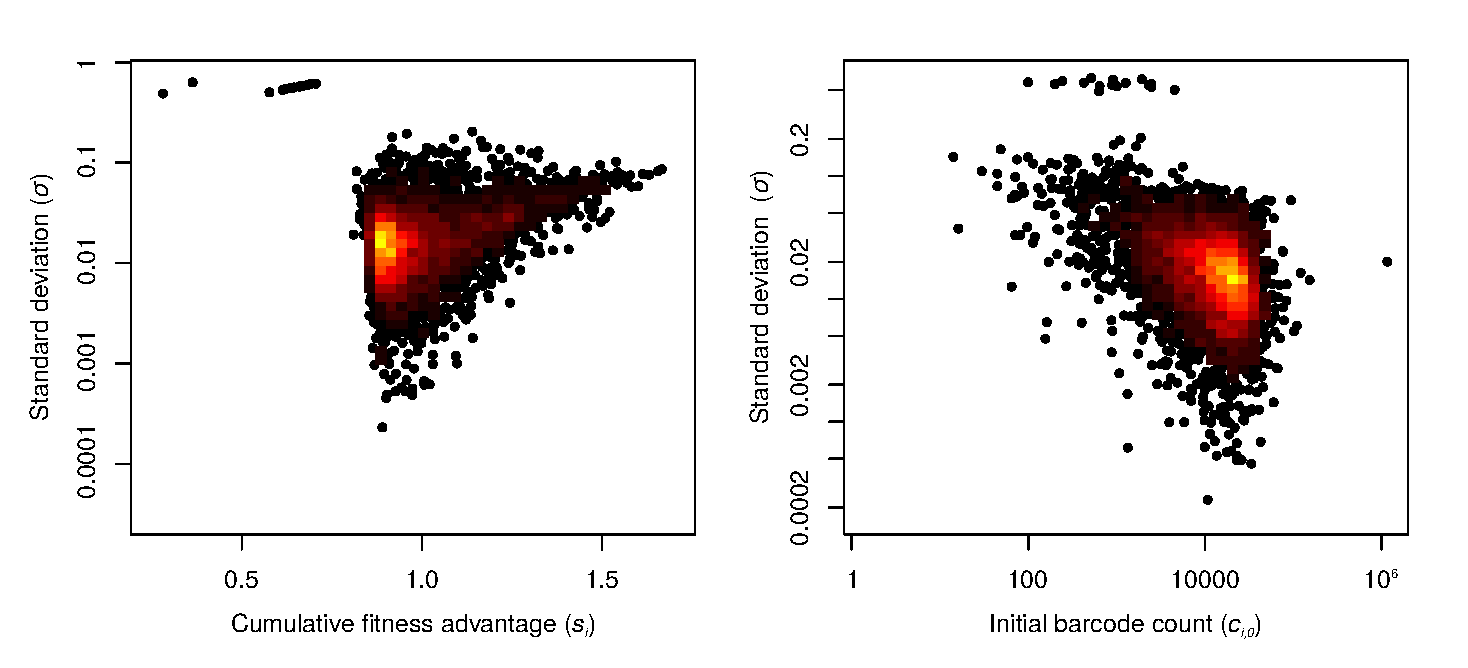
\includegraphics[width=\textwidth]{img/baldi_long.pdf}
	\caption{Comparison of fitness and initial barcode count against standard deviation. Both properties can be used as prior information to improve confidence quantification.}
	\label{fig:baldiLong}
\end{figure}


\subsubsection{A barcoded-based functional map of UBE2I}

Before further refinement in Stages 5 and 6, we wished to assess the quality of complementation scores. We first examined reproducibility of scores between technical replicates (Figure~\ref{fig:barseqValidation}A), and biological replicates (different clones carrying the same mutation; Figure~\ref{fig:barseqValidation}B).  In each case the scores were reproducible (Pearson's R of 0.97 and 0.78, respectively). We next carried out semi-quantitative manual complementation spotting assays for a subset of mutants that spanned the range of fitness scores. Complementation scores from deep mutational scanning correlated well with these small-scale tests. Indeed, agreement between the large-scale and manual scores was about the same as agreement between internal replicates of the large-scale scores (Figure~\ref{fig:barseqValidation}B,C). 

As a further sanity check, we next examined evolutionary conservation and common predictors of deleteriousness, such as PolyPhen-2~\cite{adzhubei_predicting_2001} and PROVEAN~\cite{choi_predicting_2012}.  Although each of these measures is far from perfect in predicting the functionality of amino acid changes, they should and did each correlate with functionality (Figure~\ref{fig:barseqValidation}D,E,F). Finally, we confirmed that, as expected, amino acid residues on the protein surface are more tolerant to mutation than those in the protein core or within interaction interfaces (Figure~\ref{fig:barseqValidation}G).  Taken together, these observations support the biological relevance of the DMS-BarSeq approach.

\begin{landscape}
\begin{figure}
	\centering
	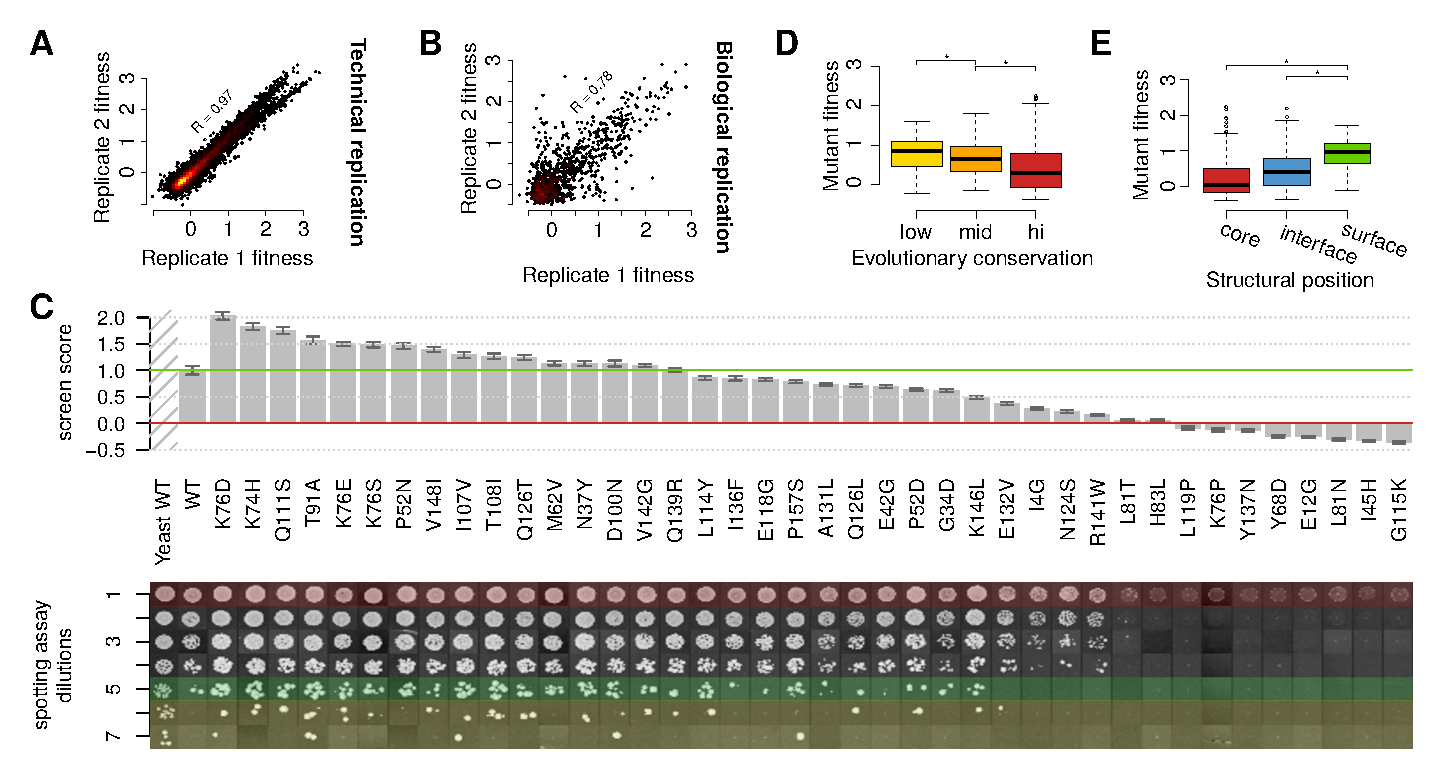
\includegraphics[width=9in]{img/barseq-validation.pdf}
	\caption{Validation of DMS-BarSeq of UBE2I. A: Correlation between technical replicates B: Correlation between biological replicates. C: Manual complementation spotting assay compared to DMS fitness measurements. D: Comparison of fitness levels for mutations at positions with low, medium and high evolutionary conservation. E:Comparison of fitness levels for mutations at positions within the hydrophobic core, at interaction interfaces, and unused surfaces}
	\label{fig:barseqValidation}
\end{figure}
\end{landscape}


\subsubsection{An alternative strategy for DMS via tiled regional sequencing}

While the DMS-BarSeq approach has many advantages (see Discussion), its performance comes at the cost of producing and maintaining an arrayed clone library, and of determining the full-length sequence of each coding region and barcode for each clone. We therefore investigated an alternative approach called DMS-TileSeq: Instead of tracking the fitness of each individual clone, we carried out \textit{en masse} measurements of the frequency of each variant in the pool before and after selection, by deep sequencing.  Sequencing was carried out for a set of short amplicon tiles that collectively encompass the complete coding region.  In this way, we can discern the impact of each mutation by observing the impact of selection on the abundance of clones carrying this mutation.

In terms of mutagenesis (Stage 1), DMS-TileSeq is identical to DMS-BarSeq.  Given the mutagenized amplicon library, the cloning step (Stage 2) was carried out by \textit{en~masse} recombinational subcloning into complementation vectors (thus skipping the step of arraying and sequencing individual clones).  This plasmid pool was next transformed \textit{en~masse} into the \textit{ubc9-ts} strain appropriate for assessing the complementation ability of \gene{UBE2I} variants. As with DMS-BarSeq, DMS-TileSeq employs pooled strains grown competitively (Stage 3) at the permissive and selective temperatures. However, instead of using barcode sequencing to determine the fitness associated with individual stains, we directly sequence the coding region from the clone population to determine the frequency of each variant in each pool (before and after selection). To overcome the problem of distinguishing mutations from sequencing errors, we divide the coding region into tiles such that each individual template molecule can be completely sequenced on both strands.  By requiring that each variant be seen on both strands, the incidence of base-calling errors can be substantially reduced. %pipeline?

An important aspect of DMS-TileSeq is that it requires the library to be sufficiently complex to ensure that the effect of a mutation is determined from enough clones and averaged over enough genetic backgrounds to be reproducible. Therefore we considered it necessary to first validate the reliability of DMS-TileSeq in comparison to DMS-BarSeq on our established UBE2I map. Correlation between DMS-TileSeq and DMS-BarSeq was comparable to the correlation observed between biological replicates of DMS-BarSeq (Supplementary Figure 2), suggesting that reproducibility of DMS-TileSeq is at least comparable to that of DMS-BarSeq. DMS-TileSeq and DMS-BarSeq showed comparable agreement with complementation scores from manual assays (Supplementary Figure 3).  Thus, DMS-TileSeq avoids the substantial cost of arraying and sequencing thousands of individual clones, while performing on par with DMS-BarSeq in terms of reliability of the functional complementation scores it produces.

\begin{figure}[h!]
	\centering
	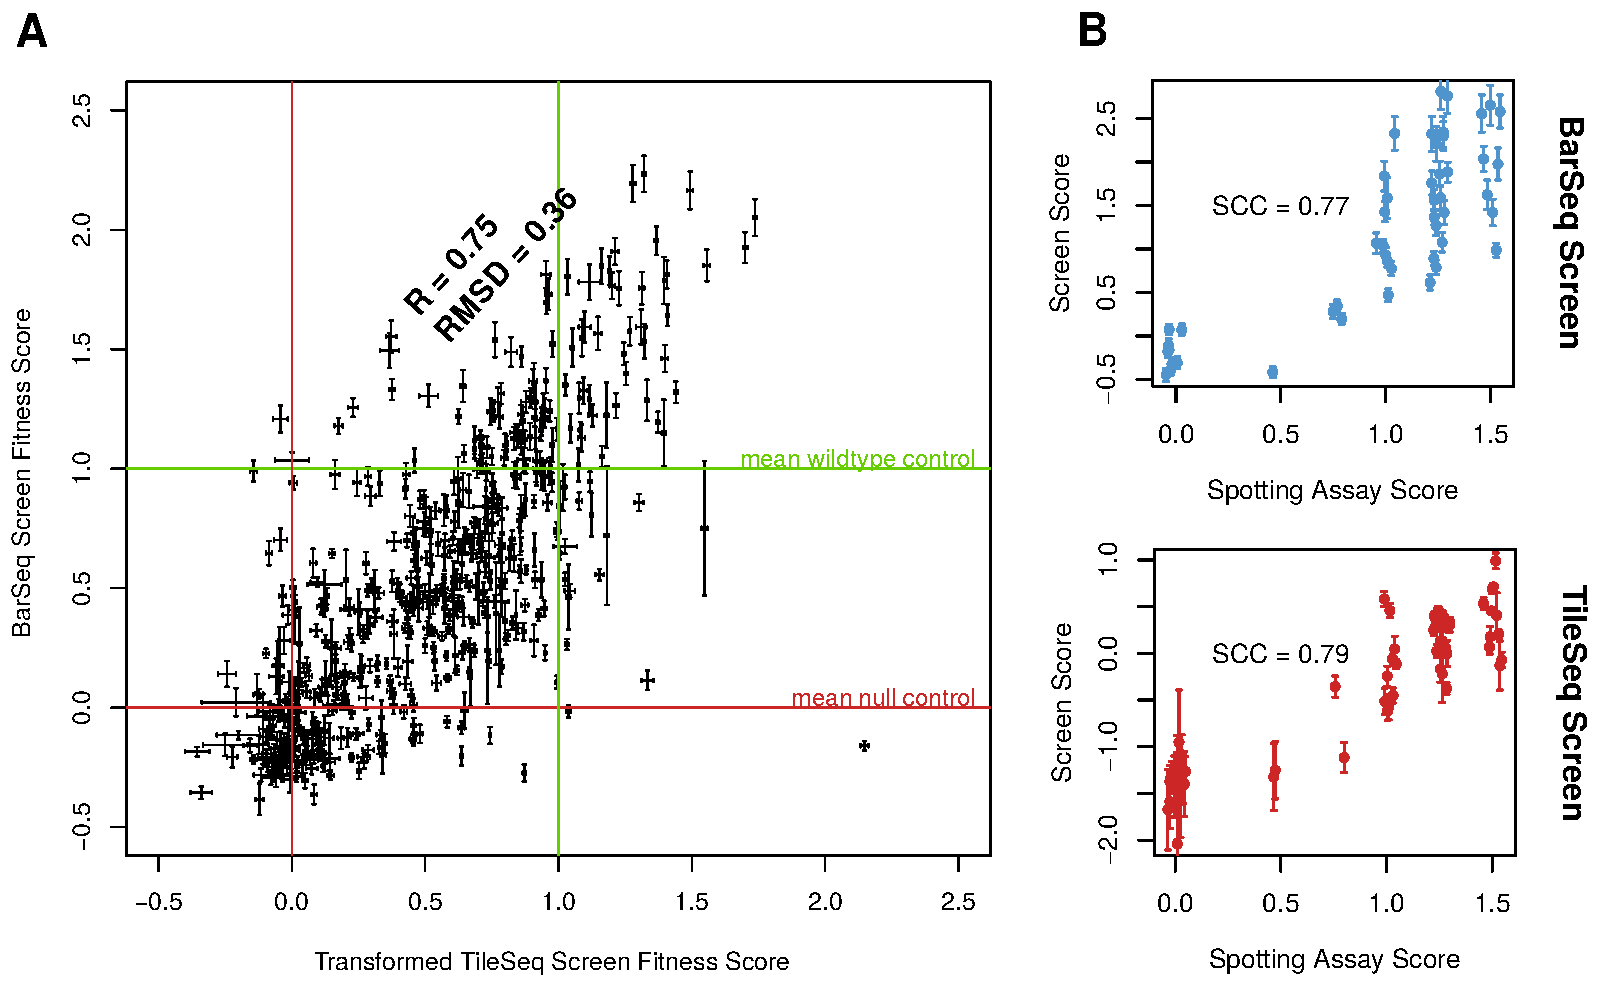
\includegraphics[width=.7\textwidth]{img/barVtile.pdf}
	\caption{Comparison of BarSeq to TileSeq scores. }
	\label{fig:barVtile}
\end{figure}

\subsection{A complete functional map of UBE2I}

Having performed two independent deep mutational scans of UBE2I using functional complementation assays, we wished to integrate both results into a single comprehensive high-quality map. To accomplish this, we first combined the results of each screening approach into a joint map.  This required bringing the maps onto the same scale. Using a regression-based transformation function, we transformed the DMS-TileSeq scores to the more intuitive scale of DMS-BarSeq (where 0 corresponds to the typical score of a null mutant and 1 corresponds to the typical score of a wildtype control). We then combined scores from the two methods, giving greater weight to more confident measurements (see Online Methods).

\subsubsection{Imputation and regularization of missing or less accurate data}

As is the case for all previously published DMS maps, our combined map contained some entries that were poorly measured or missing (e.g., because these substitutions were underrepresented in the input clone library). To fill the gaps in the map (Stage 5 in the framework), we trained a Random~Forest~\cite{breiman_random_2001} regression model using the existing measurements in the map. The features used for the model fall into four categories: intrinsic information; conservation information; chemicophysical properties; and structural properties. 

The most important intrinsic feature consists of weighted positional averages in the map. That is, for any given amino acid change, we weight all other observed effects of variants at the same amino acid position by their measurement confidence and form the average. A second intrinsic feature consists of the confidence-weighted average effect of all variants containing the amino acid change in question. Finally, as a third intrinsic feature we calculate the expected variant fitness predicted by a multiplicative model often applied to detect genetic interactions~\cite{phillips_language_1998,onge_systematic_2007}. In the absence of interaction, the fitness of a double mutant $f_{A,B}$ is expected to follow the product of the individual single mutant fitness levels $f_{A,B}\approx f_A \cdot f_B$. Thus, in cases where a double mutant $(A,B)$ and a single mutant $B$ is known, we can estimate the fitness of $A$ to be $f_A\approx \frac{f_{A,B}}{f_B}$. The model is applied to all available double mutants fitness values carrying the mutation in question in combination with available complementary single mutant fitness values. As the latter two features rely on multi-mutant fitness measurements, they can only be applied where DMS-BarSeq data is available. 

The second category of features describes evolutionary conservation. For each amino acid change in question this encompasses the corresponding BLOSUM62~\cite{henikoff_amino_1992}, SIFT~\cite{ng_predicting_2001} and PROVEAN~\cite{choi_predicting_2012} scores, and the AMAS~\cite{livingstone_protein_1993} conservation at the given position. The third set of features comprises chemicophysical properties such as mass and hydrophobicity of  the original and wildtype amino acids and the difference between the two. The fourth and final set of features consisted of structural properties of the affected amino acid residues, such as solvent accessibility and burial in interaction interfaces.

We assessed the performance of the imputation model using cross-validation. Surprisingly, we found the root-mean-squared deviation (RMSD) of imputed values to be on par with measurement error in experimentally measured data (Figure~\ref{fig:imputation}A). An examination of the prediction performance by location showed increased error in positions with lower mutation density and for variants with in above-WT fitness levels (Figure~\ref{fig:imputation}B). As an additional validation step, we performed manual complementation assays for a set of UBE2I variants that were not present in the machine learning training data set and compared the results against the predictions (Figure~\ref{fig:imputation}C), again finding a surprisingly strong agreement. Notably however, variants showing above wild-type level growth in the manual assay

\begin{landscape}
\begin{figure}[h]
	\centering
	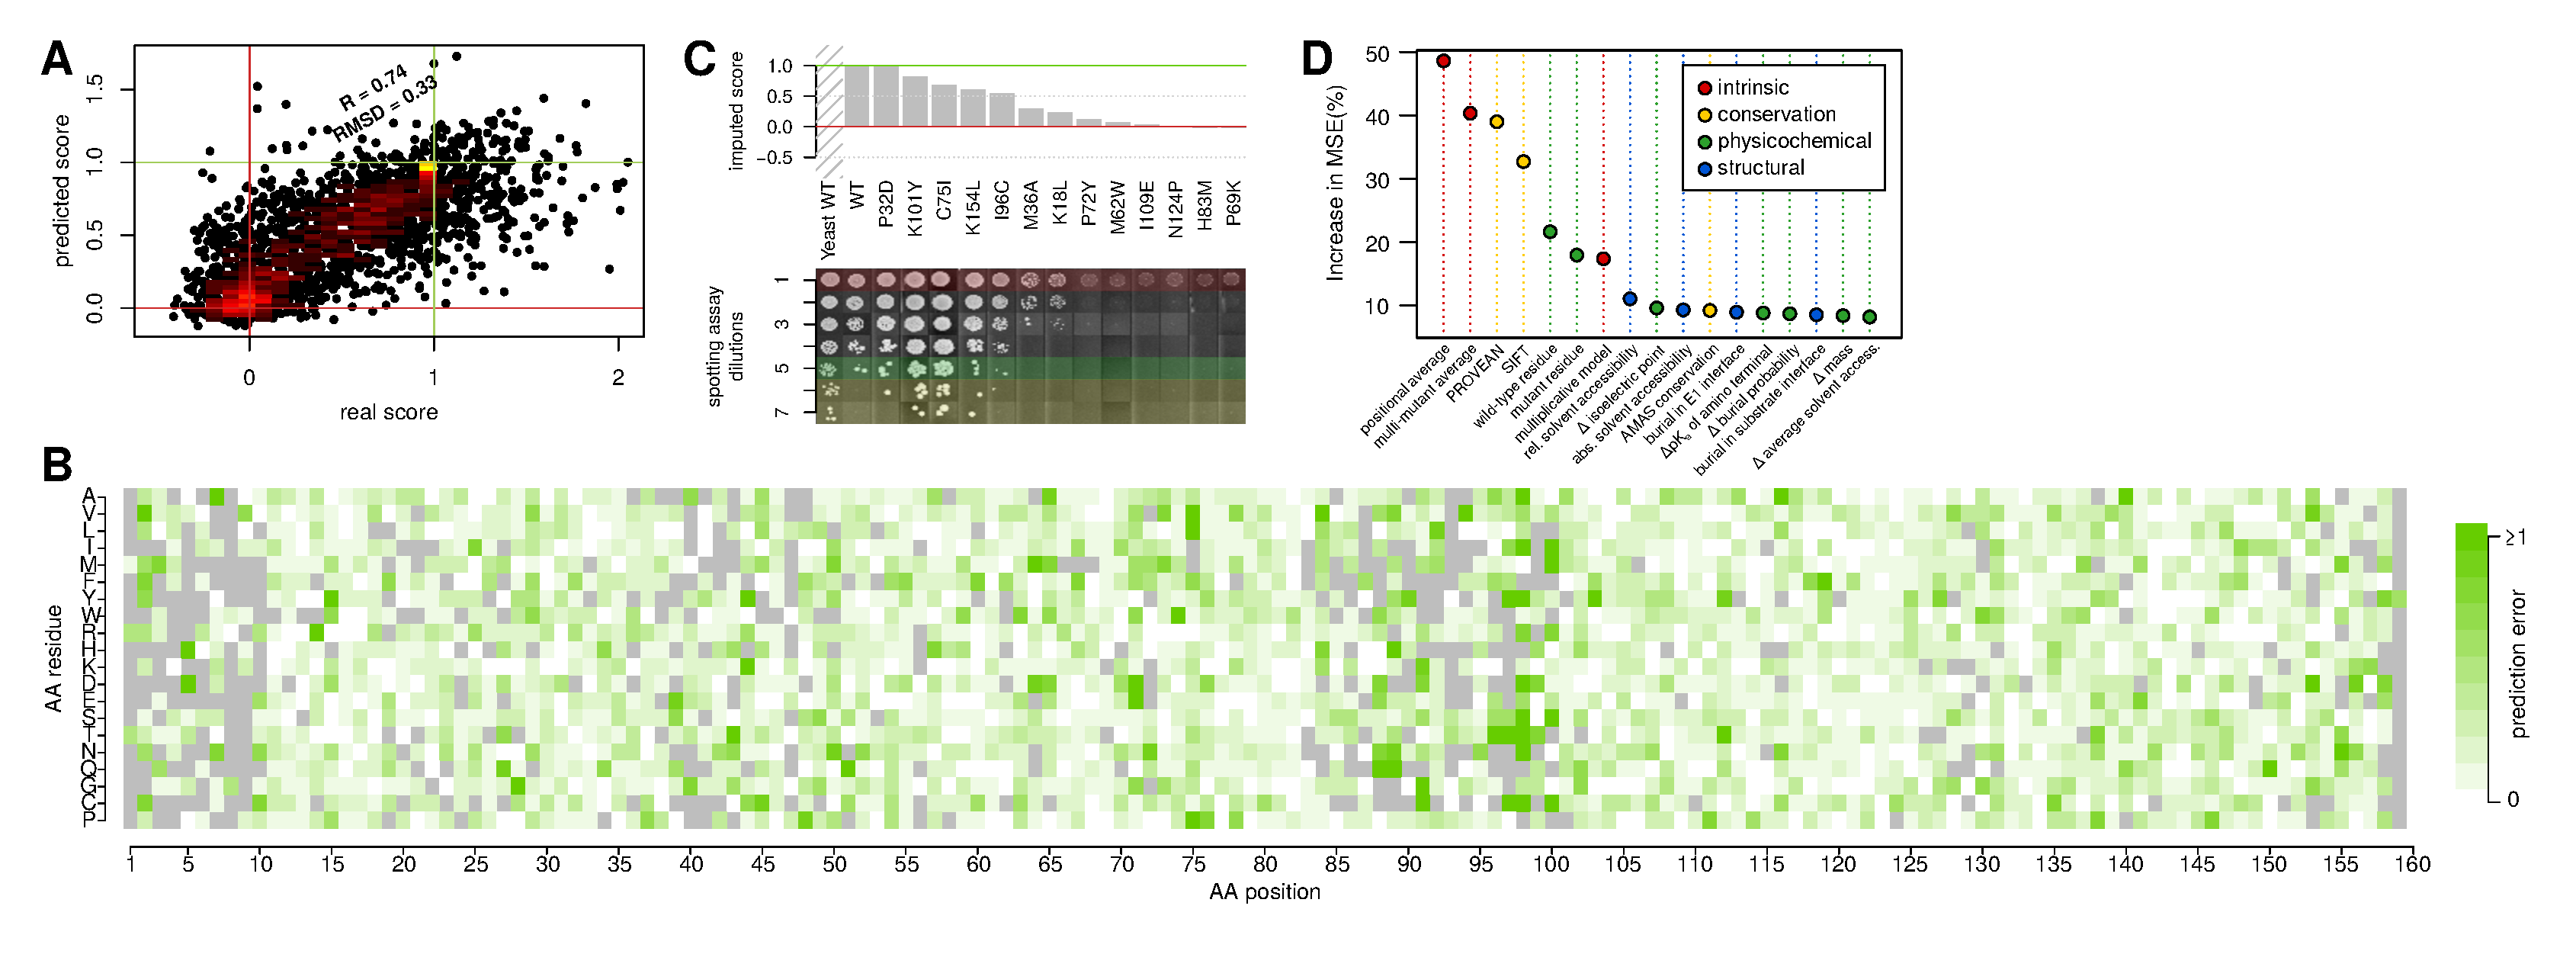
\includegraphics[width=9in]{img/imputation.pdf}
	\caption{Evaluation of Machine learning imputation. A) Cross-validation correlation between measured values and machine learning predictions. B) Cross validation prediction error landscape. C) Manual complementation spotting assay compared to machine learning predictions for an independent test set of variants not present in the training data. D) Feature importance as measured by average increase in mean squared error.}
	\label{fig:imputation}
\end{figure}
\end{landscape}

An analysis of feature importance can be performed by comparing the increase in means squared prediction error upon permuting the values of a feature in question. The analysis revealed that intrinsic features were the most informative (Figure~\ref{fig:imputation}D), with the weighed position-wise average and multi-mutant average were seen to be the two single most important features (49\% and 40\%, respectively), while the multiplicative model contributed 14\%. The second most important group was conservation information, with PROVEAN and SIFT weighing in at 39\% and 32\%, respectively.

Finally, towards stage 6 of the framework, we wished to address cases in which experimental measurements were available but less confident. We employed a regularization method, combining experimental measurements with machine-learning predicted values after dynamically weighting them according to their respective confidence levels. That means: the less confident a measurement, the stronger the regularization. 

\todo{At this point it would be nice to show off the value of the regularization, but for the unflipped UBE2I map it doesn't improve anything. The flipped maps, especially for TPK1 and CALM1 benefit much more from regularization. It would also be great if we could point to the spotting assay, but we didn't test any poorly measured clones, so we don't have any interesting data there.}

% \subsection{Evaluation and validation of the UBE2I map}
To evaluate the complete map, we once more applied manual complementation assays to a set of variants that represented the full range of fitness scores.  DMS fitness scores corresponded closely with manual assays (Figure~\ref{fig:imputation}E), thus validating our framework.  To more specifically evaluate the imputation process, we selected a smaller test set of variants (again spanning the range of scores), and recalculated imputation scores using a training set that excluded variants in this test set.  Collectively, our framework yielded a comprehensive map covering all possible missense variants, with overall quality that was on par with the highest-quality measurements from either screen alone.

The complete, refined functional map of UBE2I after imputation and regularization can be seen in Figure~\ref{fig:ube2i-map}. For comparison, additional tracks showing position-specific evolutionary conservation, secondary  structure, relative solvent accessibility and burial in protein-protein interaction interfaces are also shown.  

\begin{landscape}
\begin{figure}[h]
	\centering
	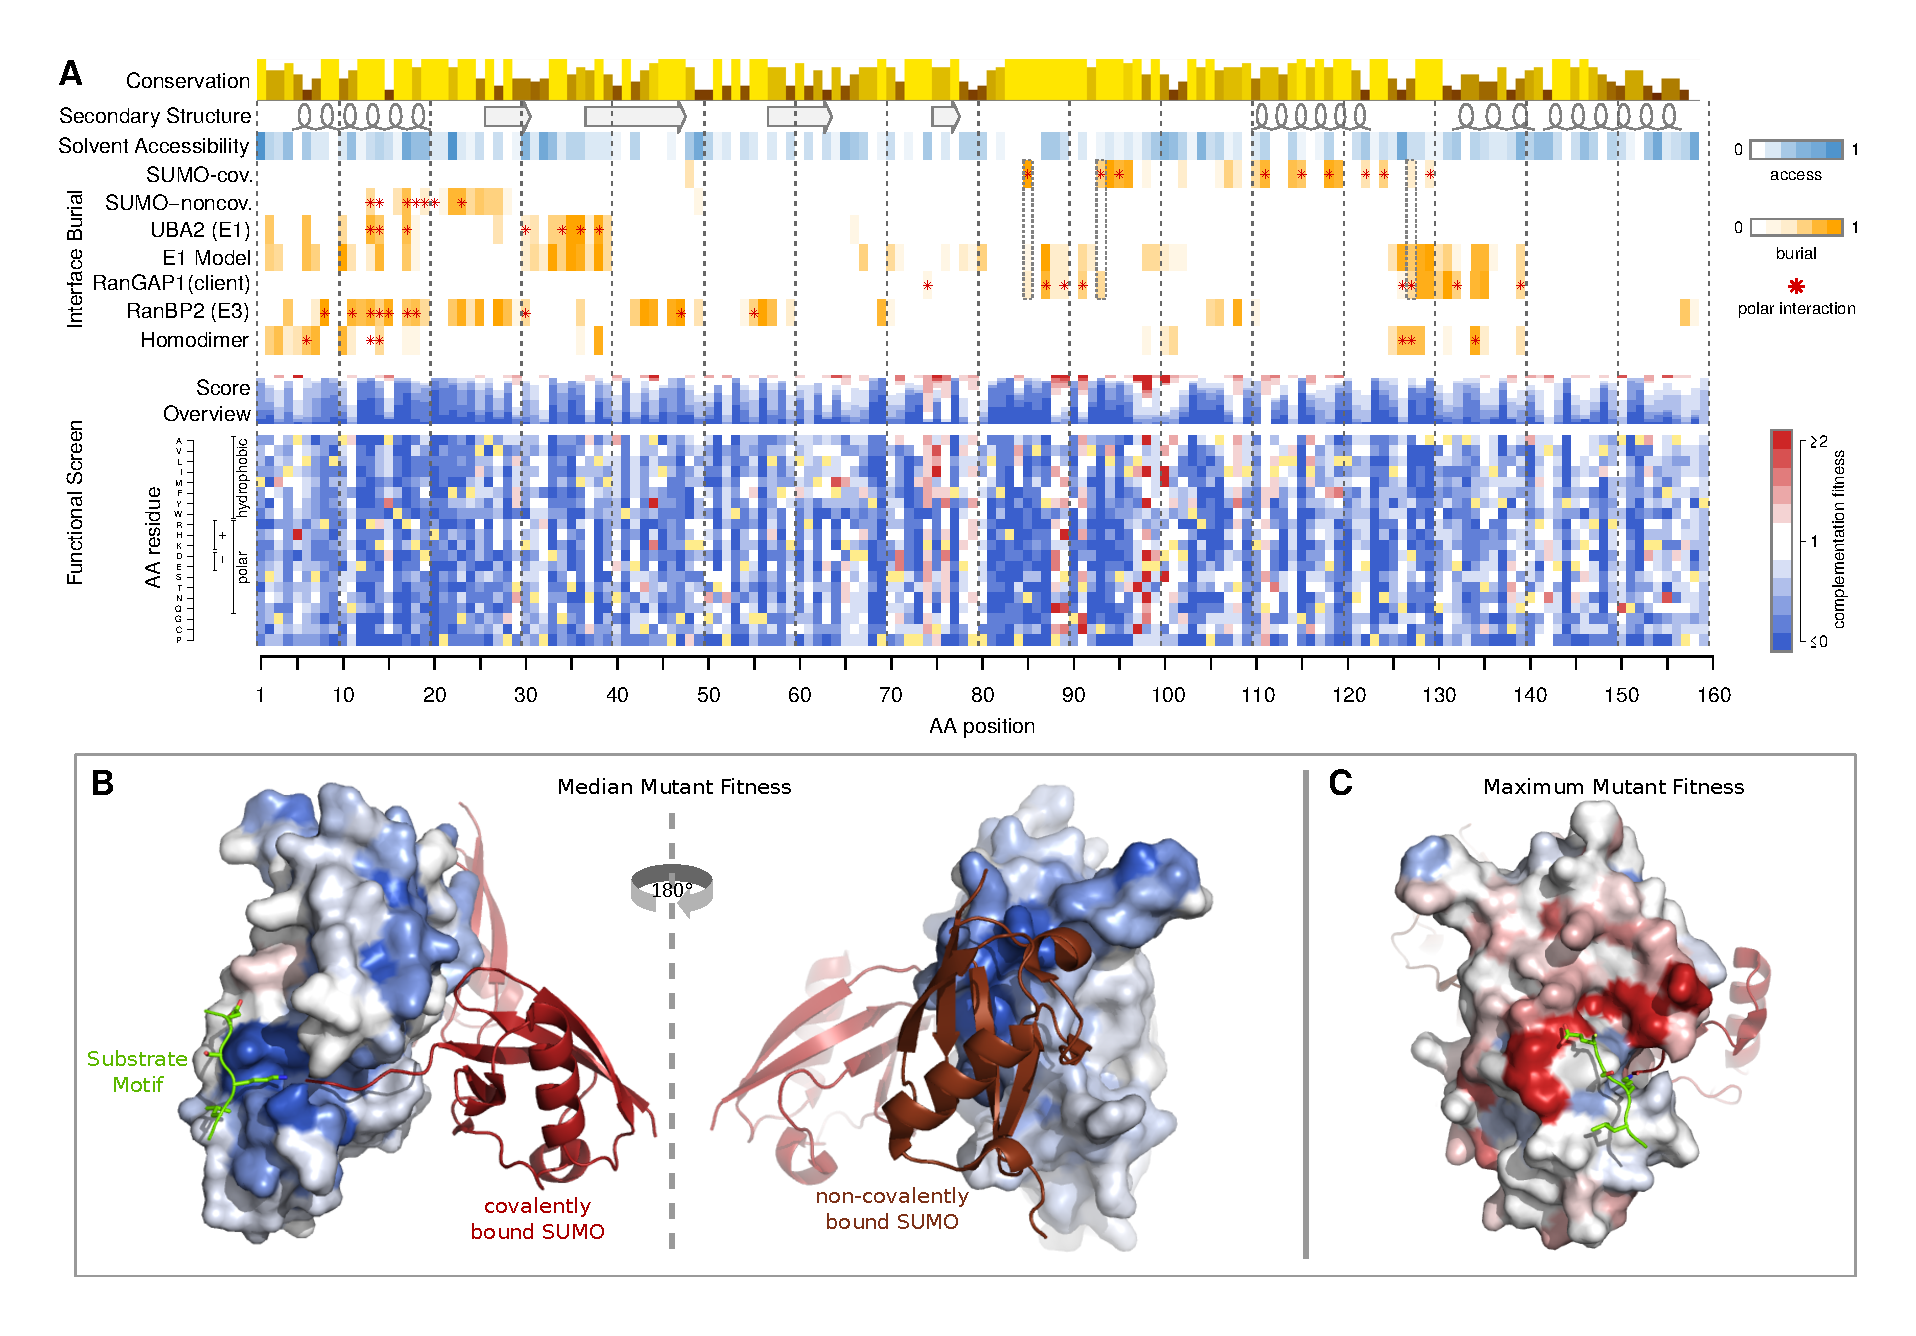
\includegraphics[width=9in]{img/ube2i_map.pdf}
	\caption{Functional map of UBE2I. From top to bottom: Position-wise evolutionary conservation (AMAS); Secondary structure; Relative solvent accessibility; Relative burial in protein-protein interaction interfaces with covalently bound SUMO, non-covalently bound SUMO, the SUMO E1 complex at two different stages of activation, the sumoylation substrate RanGAP1, the E3 RanBP2, and the UBE2I homodimer; A summary track showing the relative number of amino acid changes resulting in different fitness effects; and finally the individual amino acid change effects sorted by physicochemical groups.}
	\label{fig:ube2i-map}
\end{figure}
\end{landscape}


\section{Discussion}

Here we have demonstrated the capabilities of a new improved Deep Mutational Scanning framework that uses functional complementation in yeast to map the impact of mutations on the overall ability of a protein to function. We integrated a machine learning-based imputation and regularization strategy into the deep mutational scanning process, to allow the first DMS scans that are complete with respect to high-quality functional impact scores over the full length of a protein.

The two versions of DMS we described, DMS-BarSeq and DMS-TileSeq, each have advantages and limitations. DMS-BarSeq permits study of the combined effects of mutations located at any distance along the clone, and therefore can reveal intramolecular genetic interactions.  Mutant clones produced for DMS-BarSeq are arrayed, sequenced and indexed which can enable follow up investigation of individual variants. DMS-BarSeq can directly compare growth of any clone to null and wild type controls, resulting in an intuitive scoring scheme. However, the cost of arraying and sequencing clones for DMS-BarSeq renders it more costly and labour intensive, even given the efficient KiloSeq strategy. By contrast, the regional sequencing strategy of DMS-TileSeq is substantially more efficient, but can only analyze fitness of those double mutant combinations that fall within the same tile. 

The use of codon-replacement mutagenesis allowed us to observe a fuller repertoire of amino-acid substitutions than single-nucleotide mutagenesis would have allowed (only $\sim~30\%$ of all possible amino acid substitutions are accessible by single nucleotide mutation).  However, given that the majority of missense variants observed on individual genome are single-nucleotide variants29, one might reasonably wonder whether codon mutagenesis is worth carrying out in addition to single-nucleotide mutagenesis.  We see three arguments for using codon-level mutagenesis to reveal the impact of all 19 possible amino acid substitutions at each position:  1) a full picture of functional missense variation enables a clearer understanding of what biochemical properties required of each functionally important residue; 2) an analysis of over 60,000 unphased human exomes~\cite{lek_analysis_2016} found that each individual human harbors approximately 23 codons containing multiple nucleotide variants that collectively encode an amino acid not encoded by either single variant; 3) it seems likely that, going forward, the dominant cost of DMS will be development and validation of the functional assay, so that carrying out codon-level mutagenesis instead of (or in addition to) nucleotide-level mutagenesis has a relatively small impact on overall cost.


\section{Methods}

\subsection{Mutagenesis and library construction}

\paragraph{Oxidized nucleotide PCR: } Oxidized nucleotide PCR was performed by Jennifer Knapp as previously described by Mohan and colleagues~\cite{mohan_pcr_2011}. Primers were designed to attach attB sites to the product in preparation for Gateway cloning.

\paragraph{POPCode:} POPCode oligos are generated using the POPCodeSuite webtool which uses the following algorithm. The source code is provided on the attached storage media and can also be found online\footnote{http://dalai.mshri.on.ca/$\sim$jweile/projects/popcodeSuite/}.

POPCode mutagenesis was performed by Atina Cote, Jennifer Knapp and Marta Verby in the following steps: (i) A uracil-containing wild type template was generated by PCR-amplifying the ORF in the presence of dUTP, (ii) pooled oligonucleotides were hybridized with the template and gaps between hybridized oligonucleotides were filled with the non-strand-displacing Sulpholobus Polymerase IV (NEB) or Kapa HiFi Uracil+ DNA polymerase (KapaBiosystems) and sealed with T4 DNA ligase (NEB), (iii) the uracil-doped wild-type template was then degraded using Uracil-DNA-Glycosylase (UDG) (NEB) and the mutagenesis product was amplified with attB-sites-containing primers to allow the downstream Gateway BP cloning.

\paragraph{Library construction:} Library construction was performed by Atina Cote, Jennifer Knapp and Marta Verby. Pooled mutagenesis product carrying attB sites is cloned in to barcoded expression pHYC expression vectors in en-masse Gateway BP and LR reactions and subsequently transformed into E.coli. Automated colony picking using a BioMatrix robot was used to array $\sim$10,000 clones.

\subsection{KiloSeq and library condensation}

KiloSeq library preparation was performed by Atina Cote, Jennifer Knapp and Marta Verby. 384-well plates are prepared with PCR mastermix, where each well contains differently tagged oligos representative its respective well coordinate. A BioMatrix robot is used to stamp clones directly from the library plates into the wells. Colony PCR is performed directly in the plates using a HydroCycler. Wells across each plate are then pooled and fragmented using Nextera Tn5 tagmentation. Fragments carrying the well-specific tags within each pool are then re-amplified using primers carrying Illumina i5/i7 linkers with plate-specific indices. Finally, the products are pooled, purified and size selected.

Sequencing data is processed using a custom pipeline that runs on a high-performance computing cluster. The source code is provided on the attached storage media and can also be found online\footnote{http://dalai.mshri.on.ca/$\sim$jweile/projects/kiloseq/}.

After identification of desirable clones using KiloSeq, the selected clones were condensed into a smaller library using the BioMatrix Robot. A custom software library was developed to help program the BioMatrix Robot's picking protocol. It is provided on the attached storage media and can also be found online\footnote{http://dalai.mshri.on.ca/$\sim$jweile/projects/biomatrix/}.

\subsection{DMS-BarSeq}

\paragraph{Complementation competition experiment:} Complementation experiments were performed by Jennifer Knapp, Song Sun and Marta Verby. After pooling the barcoded \gene{UBE2I} variant library it was transformed \textit{en masse} together with barcoded null and wildtype controls into an \species{S. cerevisiae} \textit{ubc9-ts} strain. 
The pool was grown in triplicates on solid media at 25\celsius\ and 37\celsius\ to be examined at 5 different timepoints (0h, 6h, 12h, 24h, 48h), which required a total of 30 plates. At their respective timepoints, plates were scraped, OD quantified, and their barcode loci amplified with primers carrying sample-specific tags. The amplified product is then sequenced on an Illumina NextSeq 500.

\paragraph{Sequence analysis:}A custom sequenca analysis pipeline was used to identify and count individual sample tags and barcode combinations within each read. The pipeline source code is provided on the attached storage media and can also be found online\footnote{http://dalai.mshri.on.ca/$\sim$jweile/projects/screen\_pipeline/}.

\paragraph{Scoring:} A custom software was developed to perform scoring and statistical analysis. First, the relative population size for each clone is calculated by dividing each clone's barcode count by the total number of barcodes in each condition. Then the estimated absolute population size for each clone is calculated by multiplying the relative population size with the estimated total number of cells on the respective plate at the corresponding time point (obtained from OD measurements). We then treat the amount of growth between each individual time point compared to the pool average as an individual estimate of fitness, all of which act cumulatively. This is calculated as follows: Let $c_{i,t_k}^\tau$ be the barcode count for clone $i$, timepoint $t_k$ at temperature $\tau$, then $ \forall i \in \{1 \le i \le N | i \in \mathbb{N} \}$, 
$\forall k \in \{1 \le k \le 5 | k \in \mathbb{N} \}$, 
$\forall \tau \in \{25^{\circ},37^{\circ} \}$

\begin{align*}
r_{i,t_k}^{(\tau)} &= \frac{ c_{i,t_k}^{(\tau)} }{ \sum_j c_{j,t_k}^{(\tau)} }\\
P_{i,t_k}^{(\tau)} &= r_{i,t_k}^{(\tau)} \cdot P_{*,t_k}^{(\tau)} \\
\rho_{i,t_k}^{(\tau)} &= \sqrt[\uproot{5}(t_k - t_{k-1})]{\frac{P_{i,t_k}^{(\tau)}}{P_{i,t_{k-1}}^{(\tau)}}} \\
%\rho_{*,t_k}^\tau &= \sqrt[\uproot{5}(t_k - t_{k-1})]{\frac{P_{*,t_k}^\tau}{P_{*,t_{k-1}}^\tau}} \\
\phi_{i,t_k}^{(\tau)} &= \frac{\rho_{i,t_k}^{(\tau)}}{\rho_{*,t_k}^{(\tau)}}\\
\phi_{i,t_k}^\prime &= \frac{\phi_{i,t_k}^{(37^{\circ})}}{\phi_{*,t_k}^{(25^{\circ})}}\\
s_i &= \prod_k \phi_{i,t_k}^\prime \\
s'_i &= \frac{s_i - s_\text{null}}{s_\text{wt} - s_\text{null}},
\end{align*}

where $r_{i,t_k}^{(\tau)}$ is the relative population size for clone $i$ and timepoint $t_k$ at temperature $\tau$, $P_{i,t_k}^{(\tau)}$ is the absolute population size for clone $i$, timepoint $t_k$ at temperature $\tau$, $\rho_{i,t_k}^{(\tau)}$ is the measured hourly growth rate for clone $i$, timepoint $t_k$ at temperature $\tau$, $\phi_{i,t_k}^{(\tau)}$ is the fitness advantage relative to the pool growth for clone $i$, timepoint $t_k$ at temperature $\tau$, $\phi_{i,t_k}^\prime$ is the normalized relative fitness advantage for clone $i$ at timepoint $t_k$, and $s_i$ is the cumulative normalized relative fitness advantage for clone $i$. Finally, $s'_i$ is the fitness score relative to the internal null and wild type controls. This results in null-like mutants receiving a score of zero and wild type-like mutants receiving a score of one.

The scoring software is part of a larger DMS analysis package provided on the attached storage media. It is also available online\footnote{http://dalai.mshri.on.ca/$\sim$jweile/projects/popcodePipeline/doc}.

\paragraph{Error regularization: } Standard error measurements for each clone were regularized using a Bayesian method published by Baldi and Long~\cite{baldi_bayesian_2001}. A prior estimate for each measurement were obtained via linear regression over permissive read counts and fitness value. The prior is combined with the empirical standard deviation obtained from technical replication using Baldi and Long's original formula $$\sigma^2 = \frac{v_n \sigma_n^2}{v_n - 2} = \frac{v_0 \sigma_0^2 + (n-1)s^2}{v_0 + n - 2},$$ where $v_0$ represents the degrees of freedom assigned to the prior estimate, $\sigma_0$ is the prior estimate, $n$ represents the degrees of freedom for the empirical data (i.e. the number of replicates) and $s$ is the empirical standard deviation.


\subsection{DMS-TileSeq}

\paragraph{Complementation competition experiment} 
The complementation experiment was performed by Song Sun and Marta Verby in much the same way as for DMS-TileSeq, but only in duplicates rather than triplicates and only a single 48h timepoint.

\paragraph{TileSeq Sequencing:} Oligos were designed to evenly distribute across the sequence of the \gene{UBE2I} ORF in 60bp intervals and used to amplify individual sequence tiles. The resulting product was used in paired-end sequencing. A custom script was used to align reads to the \gene{UBE2I} template to identify and count variants detected by both reads in each pair. Mutation counts in each condition are normalized to sequencing depth at the respective position. Then, wildtype control counts are subtracted from the selective and permissive condition counts. Finally, the log ratio between adjusted selective and permissive counts is calculated. Error regularization was performed the same way as in DMS-BarSeq. 
The scoring procedure is implemented as part of a larger DMS analysis package provided on the attached storage media. It is also available online\footnote{http://dalai.mshri.on.ca/$\sim$jweile/projects/popcodePipeline/doc}.

\subsection{Joining of maps, imputation and regularization}

While DMS-TileSeq produces only one fitness score per variant, DMS-BarSeq in many cases contains multiple biological replicates of the same variant associated with different barcodes. To provide summary fitness values on a per-variant basis scores from biological replicates were combined using weighted means, where the weight is inversely proportional to the Bayesian regularizes standard error. The standard error assocated with the joint score is also adjusted to account for difference input fitness measurements and increased sample size.
The results from the barcoded and regional sequencing screens do not scale linearly to each other. We used regression to find a monotonic transformation function $f(x) = a \cdot e^x + b \cdot x + c$ between the two screens' respective scales. The standard deviation is transformed accordingly using a Taylor series approximation. After both datasets have been brought to the same scale we can join corresponding data points using weighted means, where the weight is again inversely proportional to the Bayesian regularized standard error. Output standard error was adjusted as before. 

Imputation of missing values was performed using RandomForest Regression~\cite{breiman_random_2001}. The following intrinsic features were generated: The confidence-weighted average fitness across mutations at the same position; The average fitness of multi-mutant clones that contain the mutation of interest; the estimated fitness according to a multiplicative model to infer mutant fitness A using a double mutant AB and single mutant B.
A second set of features was computed from differences between various chemical properties of the wildtype and mutant amino acids. These properties include size, volume, polarity, charge, hydropathy.
A third set of features is derived from the structural context of each amino acid position. This includes secondary structure, solvent accessibility, burial in interfaces with different interaction partners and involvement in hydrogen bonds or salt bridges with interaction partners. Secondary structures were calculated using Stride~\cite{frishman_knowledge-based_1995}. Solvent accessibility and interface burial were calculated using the GETAREA tool~\cite{fraczkiewicz_exact_1998} on the following PDB entries: 3UIP~\cite{gareau_determinants_2012}; 4W5V~\cite{reiter_characterization_2016}; 3KYD~\cite{olsen_active_2010}; 2UYZ~\cite{knipscheer_noncovalent_2007}; 4Y1L~\cite{alontaga_rwd_2015}. Hydrogen bonds and salt bridges candidates were predicted using FreeMol and evaluated for validity by manual inspection.
Additional features used are the PROVEAN~\cite{choi_predicting_2012} and BLOSUM~\cite{henikoff_amino_1992} scores for a given amino acid change and the evolutionary conservation of the amino acid position. Conservation was obtained by generating a multiple alignment of direct functional orthologues across many eukaryotic species using CLUSTAL~\cite{russell_clustal_2014}, which was used as input for AMAS~\cite{livingstone_protein_1993}.

The machine-learning predictions resulting generated above were also used to regularize experimental measurements of lower confidence. To this end the corrected standard error associated with each datapoint can be used to determine the weight of assigned to the measurement, as follows:
$$s_\text{joint} = \frac{1}{\frac{1}{\sigma_{\bar x}^{(0)}}+\frac{1}{\sigma_{\bar x}^{(1)}}}(\frac{1}{\sigma_{\bar x}^{(0)}} s'_0 + \frac{1}{\sigma_{\bar x}^{(1)}}s'_1),$$
where $s'_0$ is machine learning prediction, $\sigma_{\bar x}^{(0)}$ is the prediction standard error approximated by RMSD, $s'_1$ is the experimental fitness measurement, and $\sigma_{\bar x}^{(1)}$ is the assocated adjusted standard error.

The joining, imputation and regularization procedures are implemented as part of a larger DMS analysis package provided on the attached storage media. It is also available online\footnote{http://dalai.mshri.on.ca/$\sim$jweile/projects/popcodePipeline/doc}.

\subsection{Complementation spotting assays}
To validate the reliability of the fitness scores obtained during the screen, we selected a subset of clones from our original variant library that evenly covered the spectrum of scores present in the screen. After genotype verification using Sanger sequencing, \species{S. cerevisiae} \textit{ubc9-ts} strains were transformed, grown to saturation, spotted in 1/5 dilution steps and grown at the permissive and selective temperatures respectively for 48 hours in the presence of null and wildtype control. A custom software was developed to help organize and analyze image data from spotting assays. It is provided on the attached storage media and can also be found online\footnote{http://dalai.mshri.on.ca/$\sim$jweile/projects/PlateOrganizer/}.




\chapter[Expanding the atlas of human disease variants]{Expanding the atlas of variant effects in human disease genes}

\section{Introduction}

Within coming decades, millions of people will have their genome sequenced. Unfortunately, we have limited ability to interpret personal genomes, each carrying 100-400 rare missense variants~\cite{the_1000_genomes_project_consortium_global_2015} of which many must currently be classified as Variants of Uncertain Significance (VUS). For example, gene panel sequencing aimed at identifying germline cancer risk variants in families yielded VUS for the majority of missense variants~\cite{maxwell_evaluation_2016}. While functional variants can be predicted via computational tools such as PolyPhen-2~\cite{adzhubei_predicting_2001} and PROVEAN~\cite{choi_predicting_2012}, these methods can confidently detect only one third as many disease variants as are detectable by experimental assays~\cite{sun_extended_2016}. Unfortunately, experimental assays are either unavailable or economically inviable for most human disease genes. 

Recent DMS studies have provided individual maps the critical RING domain of BRCA1~\cite{starita_massively_2015} associated with breast cancer risk, and the PPAR$\gamma$ protein associated with Mendelian lipodystrophy and increased risk of type 2 diabetes~\cite{majithia_prospective_2016}. Such maps can not only identify functionality of a clinical variant accurately, but also potentially do so in advance of that variant's first clinical presentation. 

In the previous chapter, we established a framework for comprehensive high-quality screening of the functional effects across all possible missense mutations in human genes. The functional complementation assay used in the assay allows for the generation of maps that not only represent the overall functional consequences of mutations, but also serves as a common basis to make maps more directly comparable. In addition, the statistical analysis and machine learning component we introduced supports allows for high overall map quality and completeness. Using this framework we have created a complete functional map for the SUMO E2 conjugase UBE2I. Here we create a map of a second member of the Sumoylation pathway, SUMO1. We examine both map in detail before discussing the interpretation of yeast complementation phenotypes in terms of humans. 

To demonstrate the value of our frameworks in terms of clinical interpretation of variants, we proceed to add a diverse set of six new disease gene maps to our atlas: \gene{TPK1} encoding Thiamin Pyrophosphokinase 1, \gene{NCS1} encoding Neuronal Calcium Sensor 1, as well as the paralogues \gene{CALM1}, \gene{CALM2} and \gene{CALM3}, which each encode the protein Calmodulin. We evaluate the maps in terms of pathogenicity prediction and VUS reclassification.

\section{Results}

% \todo{Outline the structure of the results section}

\subsection{A functional map of SUMO E2 recapitulates known biology and poses new questions}

% \todo{Quickly recap how maps for UBE2I and SUMO1 were made}

The DMS map of UBE2I produced in the previous chapter paints a comprehensive picture of variant effects on protein function (Figure~\ref{fig:ube2i-map}). Based on the map, several observations can be made. Consistent with the results of smaller-scale biochemical studies of the SUMO E2 conjugase\cite{bencsath_identification_2002,bernier-villamor_structural_2002}, the areas most sensitive to mutation are those proximal to the active site (particularly residues 81-88, 90, 92-96, and 127-130), and the N-terminal $\alpha$-helix which mediates four protein interactions including the critical interaction with the E1 SUMO-activating complex. Within the active site, particularly strong sensitivity to mutation can be observed at the Cystein residue at position 93. This is consistent with its central role in E2 function, as it forms a thioester bond with the SUMO C-terminus~\cite{bernier-villamor_structural_2002}.

An interesting feature of the map is the alternating tendency towards damaging and benign substitutions across positions 55-65. A comparison with solvent accessibility reveals this to be caused by alternating externally and internally-oriented residues, with the latter positions constrained to be hydrophobic. This alternating tendency is also reflected in evolutionary conservation across these positions. 

All protein-protein interaction interfaces previously captured in co-crystal show increased sensitivity to mutation when compared to other surface residues (Figure~\ref{fig:ube2i_interfaces}). When comparing individual protein interaction interfaces, the most substantial fitness defects are observed in those for the E1 activating complex binding interface and the covalent and non-covalent SUMO binding interfaces (Figure~\ref{fig:ube2i_interfaces}A). While the homodimerization interface also shows significant sensitivity, the effects are not as severe as those at the E1 interface (Figure~\ref{fig:ube2i_interfaces}B). This is consistent with the Alontaga and colleagues' hypothesis regarding its involvement in SUMO chaining~\cite{alontaga_rwd_2015}, as in yeast SUMO chain formation has so far only been observed to be involved in meiosis, which is not a mechanism vital to fitness in a complementation assay. Alontaga \etal also postulate however, that non-covalent SUMO binding is necessary for SUMO chain formation. In contrast to the homodimerization interface, the non-covalent SUMO binding interface shows a very strong sensitivity to mutation. This may be due to two different reasons: (i) there is a 27\% overlap between the interface for non-covalent SUMO binding interface and the interface for E1-E2 binding, which is among the most sensitive surfaces in UBE2I; and (ii) non-covalent SUMO binding also plays an important role as an adapter for many E3 proteins~\cite{cappadocia_structural_2015}.


\begin{figure}[h!]
	\centering
	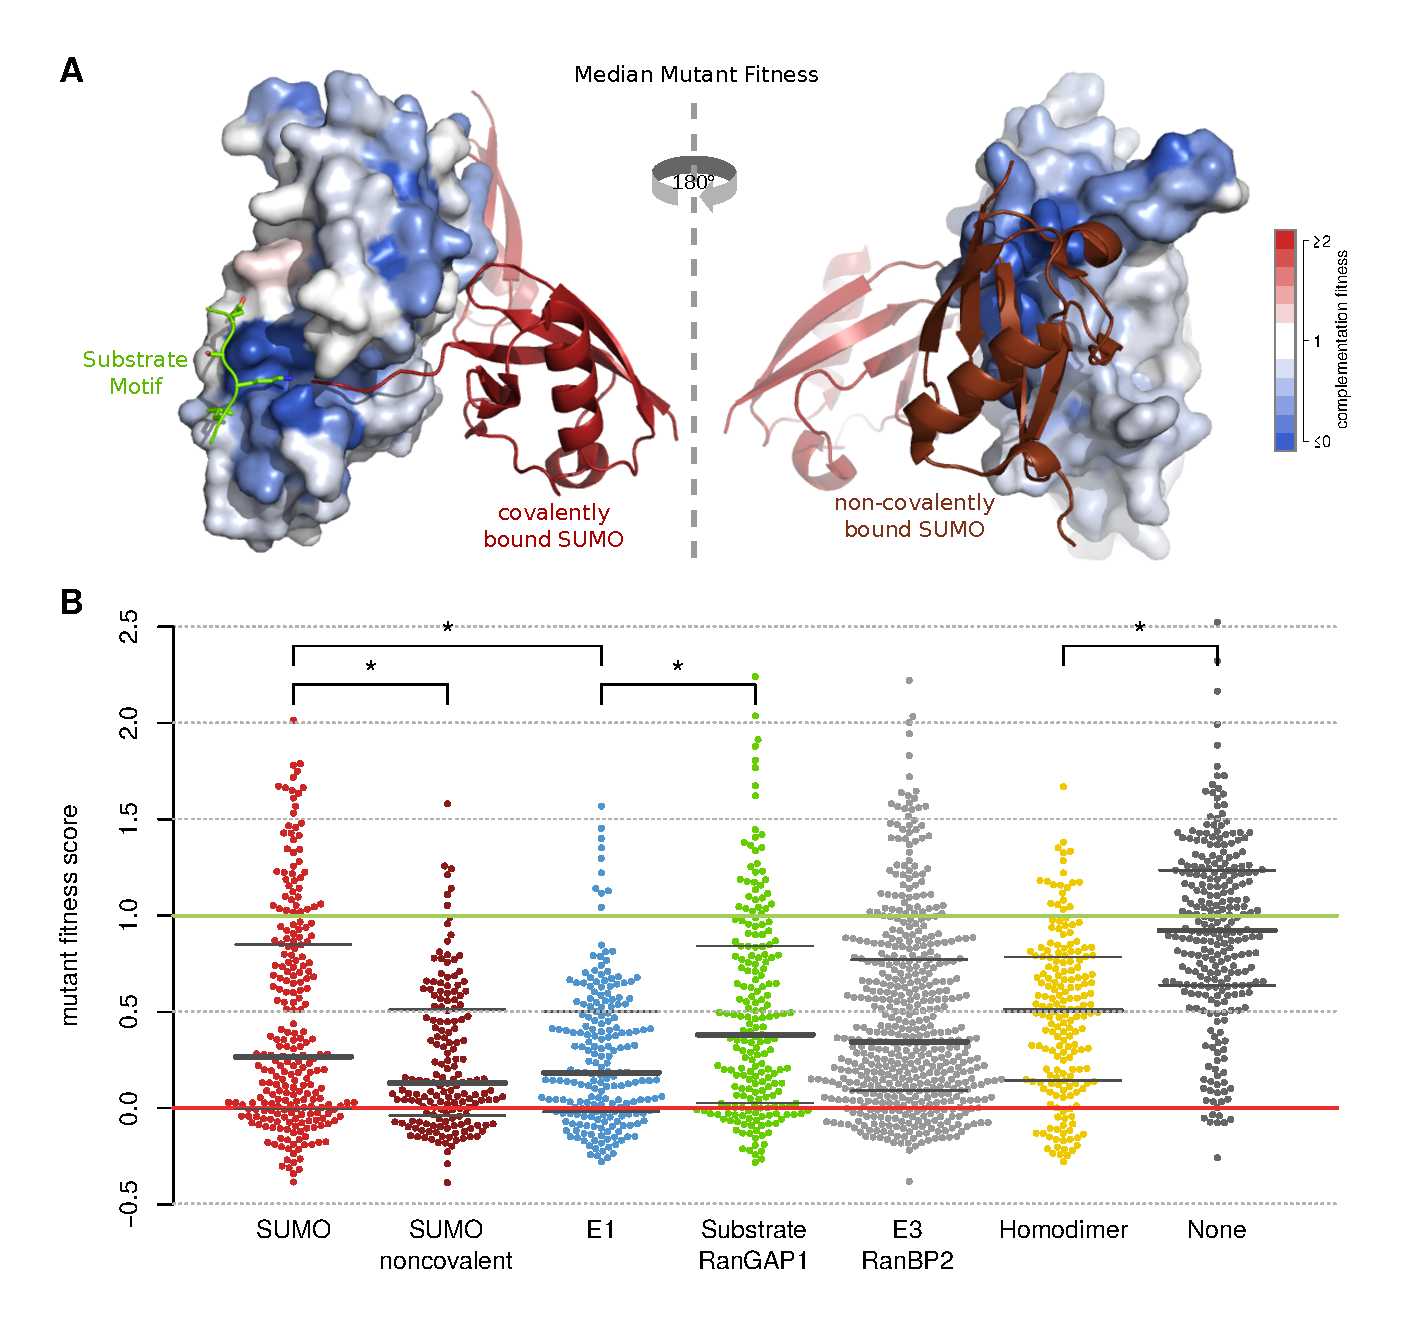
\includegraphics[width=\textwidth]{img/ube2i_interfaces.pdf}
	\caption{Complementation fitness of mutations at interaction interfaces. A) Median mutant fitness mapped to the crystal structure of UBE2I. The $\Psi$KXE substrate recognition motif is shown as green stick model, covalently and non-covalently bound SUMO are shown as crimson and brown cartoon model, respectively. B) Mutant fitness scores distributions for residues at different interaction interfaces. }
	\label{fig:ube2i_interfaces}
\end{figure}

Another interesting observation can be made with respect to a known phosphorylation site on the surface of UBE2I. Su and colleagues previously discovered that phosphorylation of Serine 71 via the Cyclin-dependent Kinase CDK1 results in sumoylation hyperactivity~\cite{su_phosphorylation_2012}. Our map shows that substitutions with phosphomimetic residues at this position lead to hyperactive complementation, consistent with Su~\etal's observations. Furthermore, other residues amenable to phosphorylation are also tolerated, while hydrophobic replacements are generally deleterious (Figure~\ref{fig:phosphosite}).


\begin{figure}
	\centering
	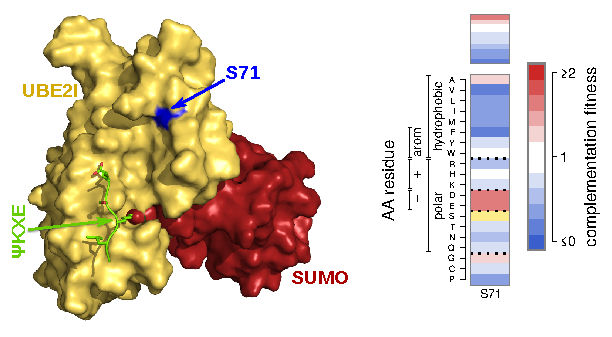
\includegraphics[width=\textwidth]{img/phosphosite.pdf}
	\caption{Phoshporylation site of UBE2I shows hyperactive complementation when mutated to phosphomimetic residues.}
	\label{fig:phosphosite}
\end{figure}


\subsubsection{Substrate specificity shifts and E2 hyperactivity}

Intriguingly, many sites show fitness that is better than wildtype (e.g., positions 74, 76, 88, 89, 91 and 98). Manual functional complementation spotting assays confirmed that complementation with these mutants allows greater growth than does the wild type human protein, but resemble more closely the growth at the permissive temperature for the \textit{ubc9-ts} strain (Figure~\ref{fig:hyperactive}A). One might be tempted to interpret these cases as reversions to residues present in the yeast protein. However, a comparison of fitness score distributions between changes to S. cerevisiae  residues and those occurring in the distant species \species{Dictyostelium~discoideum} (amoeba) or \species{Drosophila~melanogaster} (fly) showed no significant difference (Figure~\ref{fig:hyperactive}B). Recognizing that in this assay, human UBE2I must function with the yeast versions of other sumoylation pathway members, it stands to reason that some substitutions could be adaptive by improving compatibility with yeast interaction partners. A comparison with co-crystal structure data~\cite{gareau_determinants_2012} shows that many of the apparently-adaptive residues are located on the surface facing the general direction of the substrate, with some being in direct contact with the substrate's sumoylation motif (Figure~\ref{fig:hyperactive}C). This suggests a possible adaptation via improved recognition of substrates for which sumoylation is most important for yeast growth. Indeed, \textit{in vitro} sumoylation assays performed previously for a small number of UBE2I mutants revealed increased sumoylation for some substrates~\cite{bernier-villamor_structural_2002}. Comparing our map with these sumoylation assay results, we confirmed that above-WT complementation levels were enriched for cases of substrate specificity shift (Figure~\ref{fig:hyperactive}D). \todo{This needs to be discussed in more detail}


\begin{figure}[h!]
	\centering
	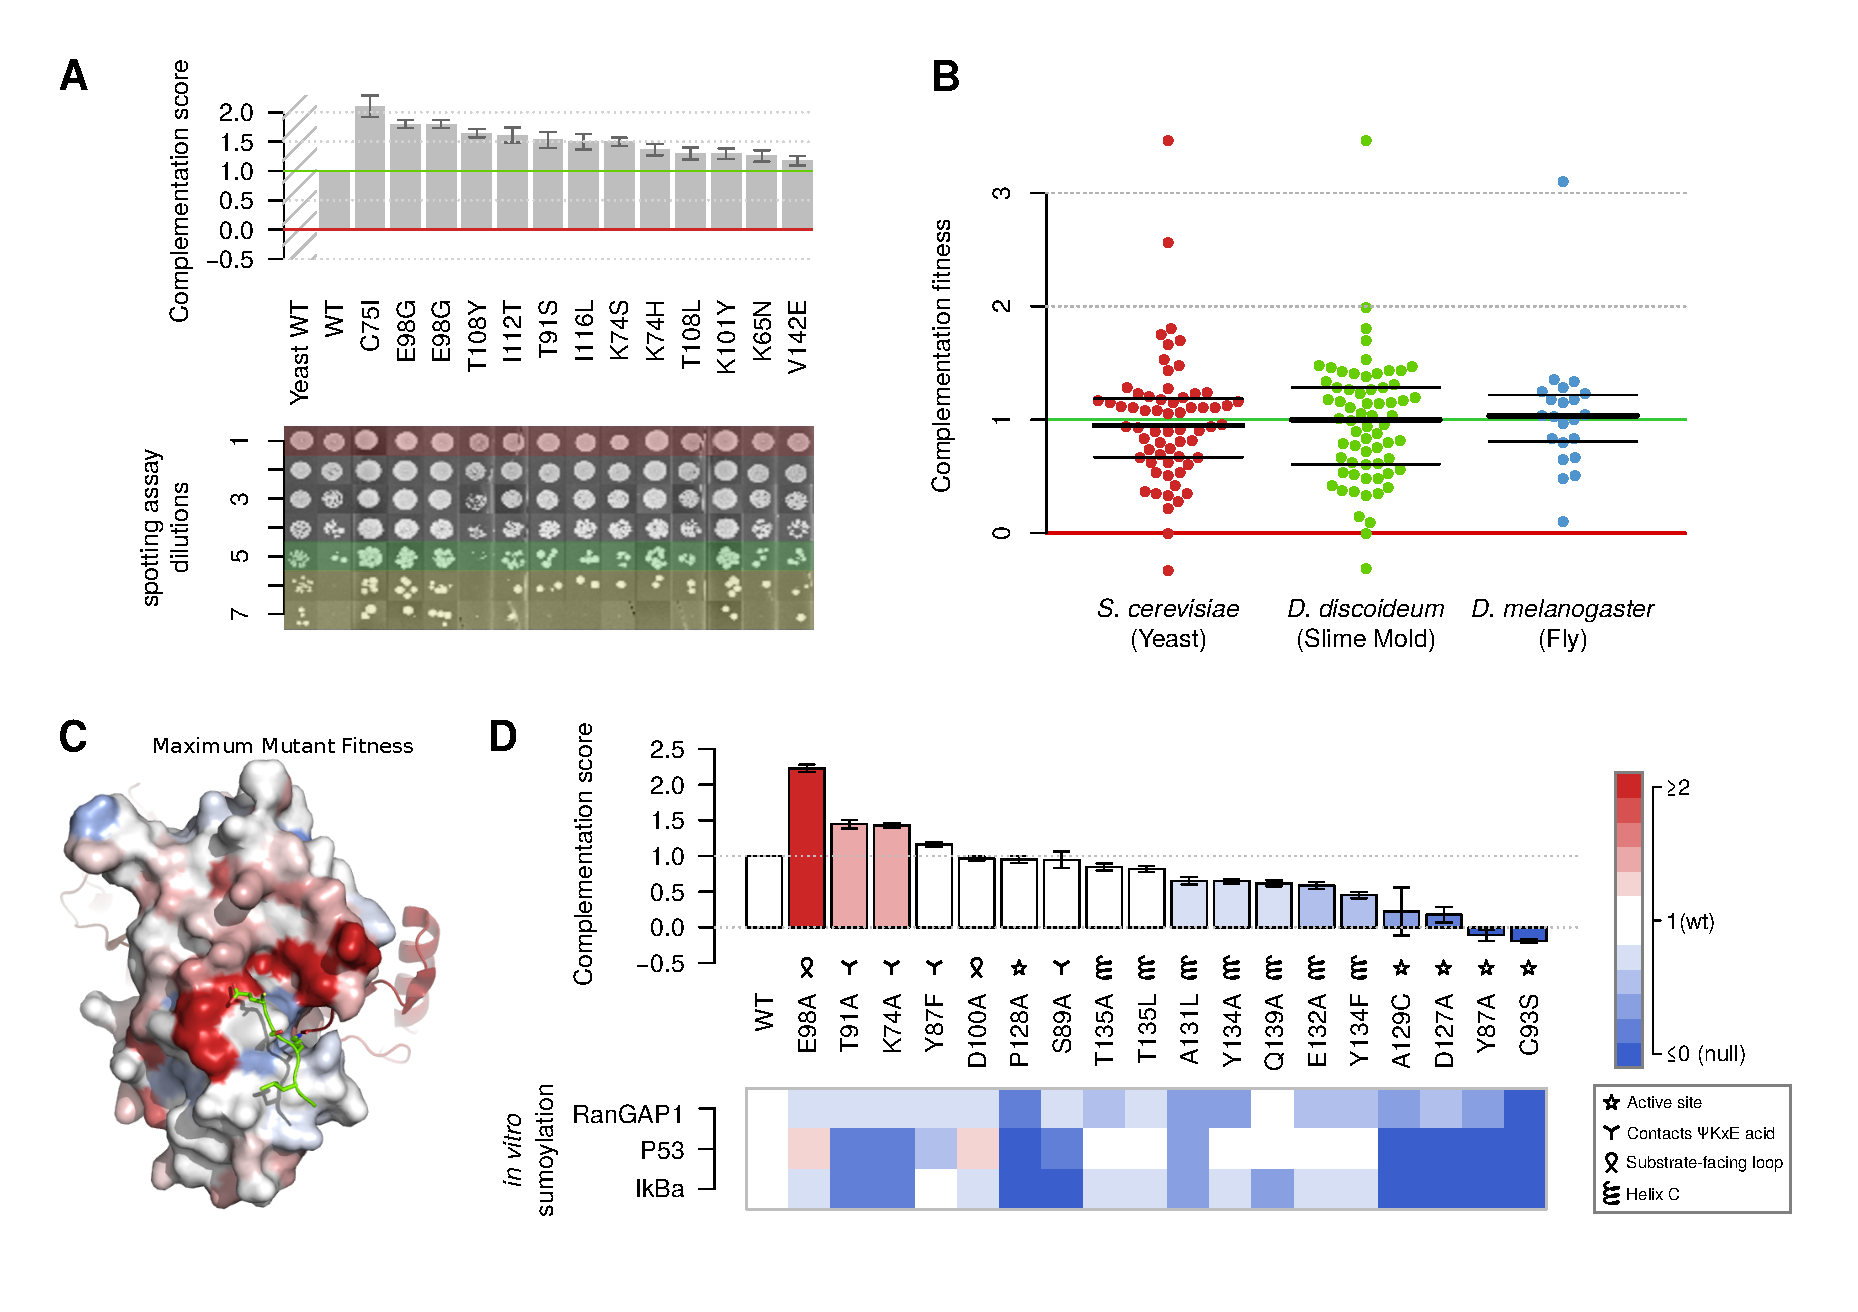
\includegraphics[width=\textwidth]{img/hyperactive.pdf}
	\caption{Hyperactive complementation in UBE2I. A) Variants scoring higher than the wildtype controls show stronger growth in manual complementation spotting assays and resemble the WT yeast. B) Distribution of scores for changes to residues naturally occurring in yeast, amoeba and fly are not significantly different from each other. C) Maximum mutant score mapped to amino acid positions on UBE2I structure. Hyperactive mutations are clustered at the substrate recognition site. Structure data from \texttt{PDB:3UIP}~\cite{gareau_determinants_2012} D) \textit{In vitro} sumoylation assay data from Bernier-Villamor~\etal~\cite{bernier-villamor_structural_2002} in comparison to the complementation fitness scores.}
	\label{fig:hyperactive}
\end{figure}


As Figure~\ref{fig:hyperactive}D shows, substrate specificity does not paint a complete picture of the mechanisms potentially underlying hyperactive complementation. A particularly interesting exception can be observed at residues A15 and T108. Both residues harbor hyperactive mutations but do not face towards the substrate. Instead, they form part of the interface with the E3 SUMO ligase RanBP2, and flank a small cavity on UBE2I's surface into which RanBP2 inserts a phenylalanine residue upon binding~\cite{gareau_determinants_2012}. Changing either A15 or T108 into aromatic residues results in a large fitness increase (Figure~\ref{fig:pi-stack}). This may be the result from the emergence of a $\pi$-stack interaction that strengthens E2-E3 binding.

\begin{figure}[h!]
	\centering
	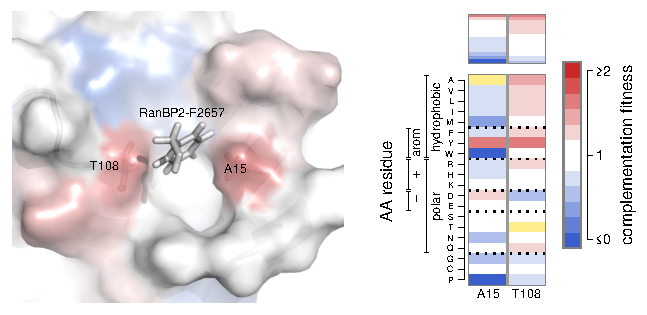
\includegraphics[width=\textwidth]{img/pi-stack.pdf}
	\caption{Potential de-novo pi-stack interaction between UBE2I and the E3 RanBP2. Structure data from \texttt{PDB:3UIP}~\cite{gareau_determinants_2012}}
	\label{fig:pi-stack}
\end{figure}

It is unclear how to interpret the effect of mutations that enhance growth in the yeast complementation assay. If fitness measured in the assay is directly proportional to fitness in the real biological context, then these enhancing mutations would be beneficial. However one can also imagine an alternative scenario in which activity-enhancing mutations are deleterious in the real biological context. To objectively distinguish between these possibilities, we collaborated with Jesse Bloom to employ a method he recently published that leverages likelihood-based phylogenetics to quantitatively compare how well different experimental measurements represent actual evolutionary constraints in nature~\cite{bloom_experimentally_2014,bloom_identification_2017}. We compared three models relating the experimental fitness to the evolutionary preference for a mutated amino-acid sequence: (a) the evolutionary preference was directly proportional to the untransformed experimental fitness; (b) the preference had a ceiling at the wildtype experimental fitness (values greater than 1 were set to 1); or (c) the preference was set to the reciprocal of fitness for mutations with greater-than-wildtype scores, corresponding to a deleterious effect of enhancing mutations. Dr. Bloom kindly provided the phydms software~\cite{bloom_identification_2017} to test which of these three approaches best described the evolutionary constraint on a set of naturally occurring UBE2I homologs, using fitness scores that excluded conservation features from the regularization process, to avoid the circularity of using natural sequence data when deriving the scores. As shown in Table~\ref{tab:phydms}, the best fit is achieved using the model that assumes that enhancing mutations are deleterious. This result provides objective support for the idea that mutations that enhance activity above wildtype levels in the complementation assay are actually deleterious in a real biological context.

Based on these observations we reinterpreted cases of hyperactive complementation in our map as deleterious and repeated the imputation and regularization procedure. This lowered the cross-validation RMSD substantially, from $0.33$ to $0.24$.

\begin{table}[h!]
	\centering
	\caption{Comparison of different models for the effects of hyperactivating mutations. AIC: Akaike Information Criterion\newline}
	\begin{tabular}{l r}
Model & \parbox[t]{1in}{$\Delta$AIC relative\newline to best model}\\ \hline\hline
Hyperactive mutations as deleterious & 0\\
Hyperactive mutations as WT & 27.7\\
Hyperactive mutations as beneficial	& 60.6	
	\end{tabular}
	\label{tab:phydms}
\end{table}



\subsubsection{Intragenic epistasis and compensatory mutations}

Full-length UBE2I clones generated for DMS-BarSeq analysis often encoded more than one amino acid change. Multi-mutant clones offer the opportunity to search for intragenic genetic interactions. Genetic interaction is defined when a combination of mutations yields an unexpected phenotypic effect, so that identifying genetic interactions requires that we model the phenotype expected from a combination of mutations, given the single-mutant effects.  Here we used a previously-described multiplicative model~\cite{phillips_language_1998,onge_systematic_2007} in which genetic interaction is measured as $\varepsilon_{ij} = f_i \cdot f_j - f_{ij}$, where $f_i$ and $f_j$ represent single mutant fitness and $f_{ij}$ represents double mutant fitness scores. Most double mutants (71\%) did not show a significant deviation from $\varepsilon_{ij} = 0$ under this model, while 328 position pairs did show significant genetic interaction (Figure~\ref{fig:epsistasis}, see Methods). Of particular interest are compensatory interactions, i.e. cases where a double mutation is more fit than either of the component single mutations.  Where compensatory residues are proximal in the protein structure, the combination of two mutant residues may be able to re-establish a physical interaction that was lost in each of the single mutants. Although the majority of genetically interacting sites were not proximal in the structure (Figure~\ref{fig:epsistasis}B), there were interesting exceptions. For example, the I4T-P69S double mutant appears to exhibit compensatory behaviour: In the wild type structure, the van-der-Waals radii of the two residues are in direct contact (Figure~\ref{fig:epsistasis}C). Either mutation alone would be expected to destabilize the hydrophobic interaction between isoleucine and proline.  However, In the double mutant, hydroxyl groups on the two residues could adopt a hydrogen bond that re-establishes interaction and re-stabilizes the fold (Figure~\ref{fig:epsistasis}D).

\begin{figure}[h!]
	\centering
	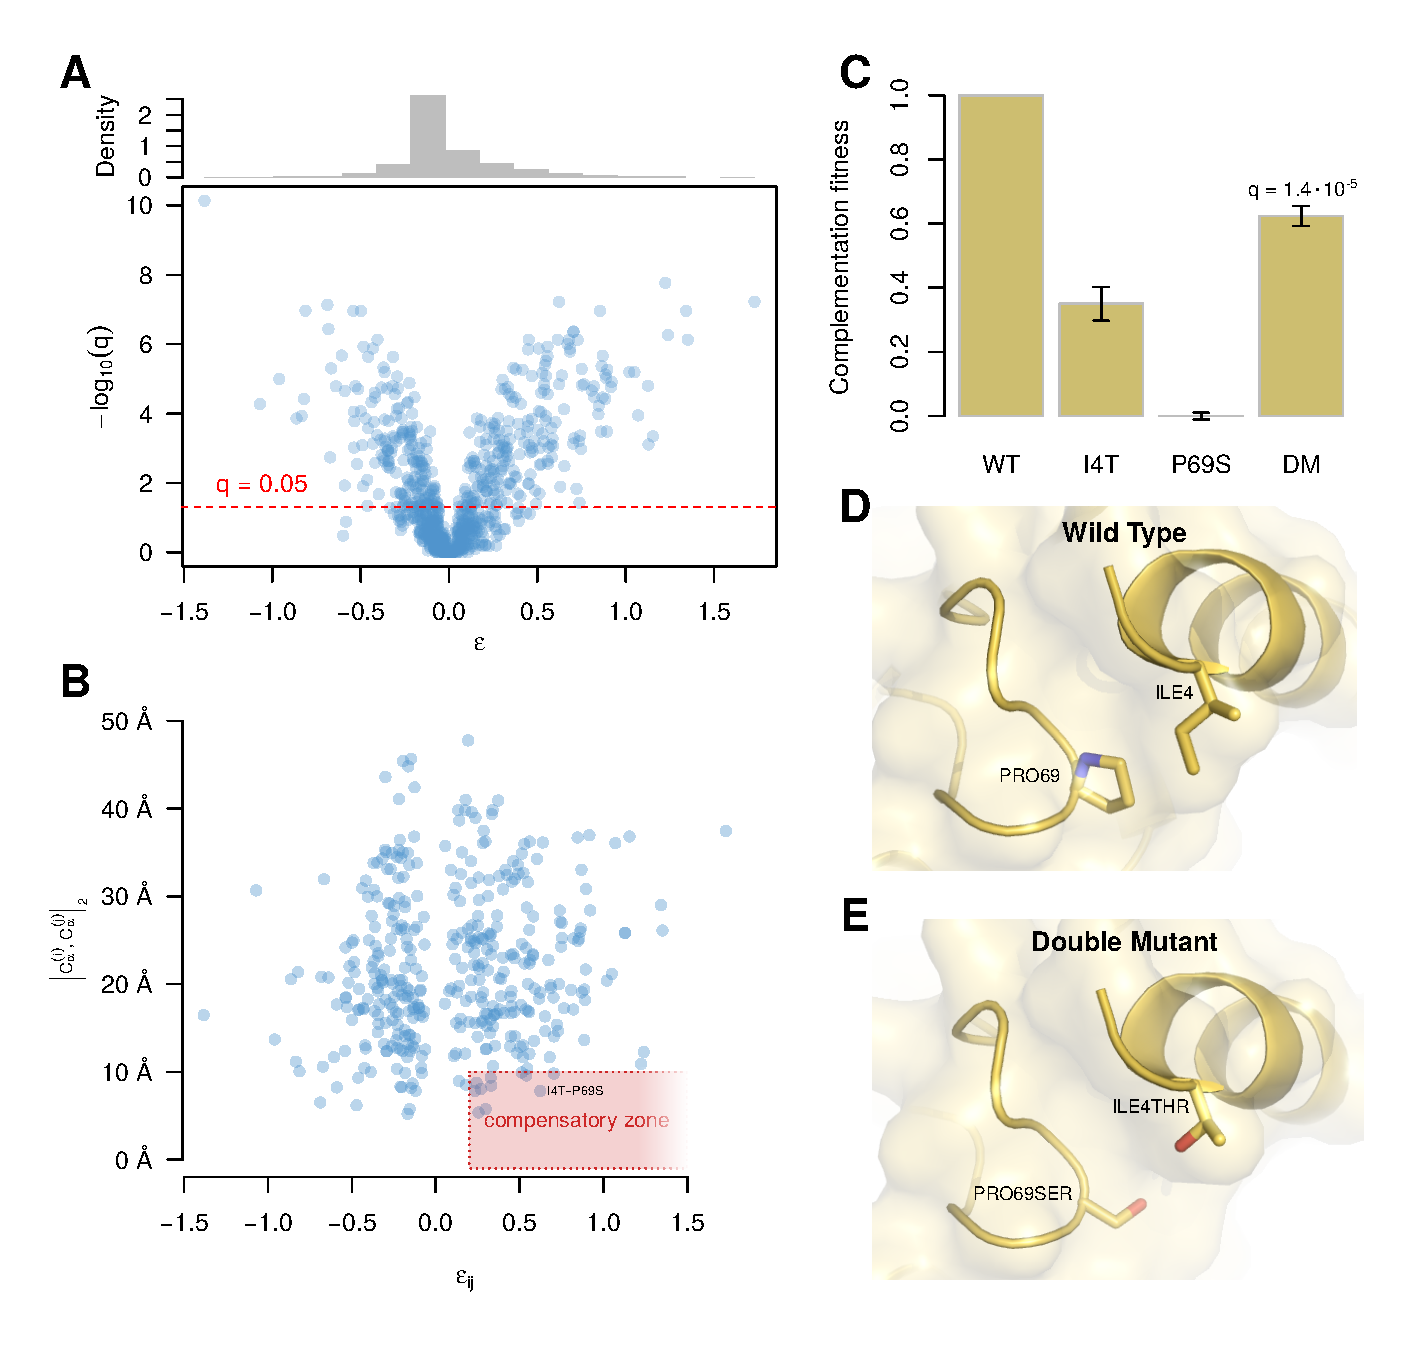
\includegraphics[width=\textwidth]{img/epistasis.pdf}
	\caption{Epistasis}
	\label{fig:epsistasis}
\end{figure}


\subsection{A comparison of complementation and Y2H reveals a interaction interface}

An important factor behind the choice of UBE2I as a testing ground for our DMS framework was the mechanistic complexity of the Sumoylation pathway, in which the central component UBE2I engages in many different protein-protein interactions. Having examined the relative importance of its known interaction interfaces we wished to evaluate the possibility of detecting new interfaces. To this end, we adapted our framework to use a Y2H assay in the selection step.

We explored the set of previously identified Y2H interactions of UBE2I and found its interaction with the Special AT-rich sequence Binding protein SATB1, a sumoylation target, to be the strongest interaction signal. We used DMS-BarSeq to map the effects of UBE2I variants on the interaction and compared the results to those of the complementation assay. Although too few variants in the Y2H screen were measured with high enough confidence to perform reliable imputation, we were able to identify a \todo{find number} variants that specifically disrupted the UBE2I-SATB1 binding without affecting its overall function as measured by the complementation assay. Figure~\ref{fig:y2hVScompl}A highlights these residues on the surface of UBE2I, which may determine the specificity of the UBE2I-SATB1 interaction. Consistent with SATB1's known role as a sumoylation target, the residues are clustered near the known substrate recognition and binding surface. Intriguingly, we also found a number of residues within UBE2I's hydrophobic core, that upon mutation to alternative hydrophobic residues resulted in a disruption of UBE2I-SATB1 binding (Figure~\ref{fig:y2hVScompl}B). The fact that these residues are physically close to the locations of surface residues with similar behaviour may indicate that mutations at these positions could result in subtle shifts of UBE2I's fold that disrupt the SATB1 binding interface without affecting other functions.

%%%%%%%%%%%Figure for Y2H vs Compl. %%%%%%%%%%


\subsection{A functional map for SUMO1}

Using the DMS-TileSeq version of the framework established in the previous chapter we also created a complete functional map for SUMO1 (Figure~\ref{fig:sumo-map}A). Out of the 1919 possible amino acid changes, fitness effects for 1700 (89\%) were measured directly in the complementation competition experiment. The remaining 11\% were obtained through imputation, which achieved a cross-validation RMSD of 0.25, a performance very similar to that of the UBE2I map.

The most immediately apparent feature of the SUMO1 map was the strong enrichment for neutral substitutions within the first 20 amino acid positions, which is consistent both with the low level of evolutionary conservation for this region and its annotation as a disordered region. The last four amino acid positions appeared similarly insensitive to mutation, consistent with the cleavage of this region by SENP proteases during SUMO maturation. By contrast, other residue positions were strongly sensitive to mutation, including many inward-facing residues that are apparently constrained to be hydrophobic. As expected, the C-terminal diglycine, directly preceeding the last four cleaved residues, is also very sensitive to mutation, as it is required for the covalent binding of SUMO to the E1, the E2 and to the sumoylation target protein.Interestingly, except for the C-terminal diglycine, the residues that directly touch the E2 during covalent binding are not as sensitive (Figure\ref{fig:sumo-map}B). This may be due to  SUMO being force-fed to the E2 by the E1 activating complex and the thioester bond it forms with the E2's cystein \#93 is all that is needed to maintain the complex. By contrast, residues in the interface for non-covalent E2 binding are much more sensitive (Figure\ref{fig:sumo-map}C). Especially leucine \#80 and methionine \#82 appear to be important

Other strongly constrained residues are core members of interaction interfaces. These include the central phenylalanine 36 in the SUMO recognition motif (SRM) interface; glycine 68, which forms the apex of a tight turn within the interface with de-sumoylation enzymes, as well as the E1 and E2 proteins; and leucine 80, which is part of the interface with non-covalently bound E2. 

\begin{figure}[h!]
	\centering
	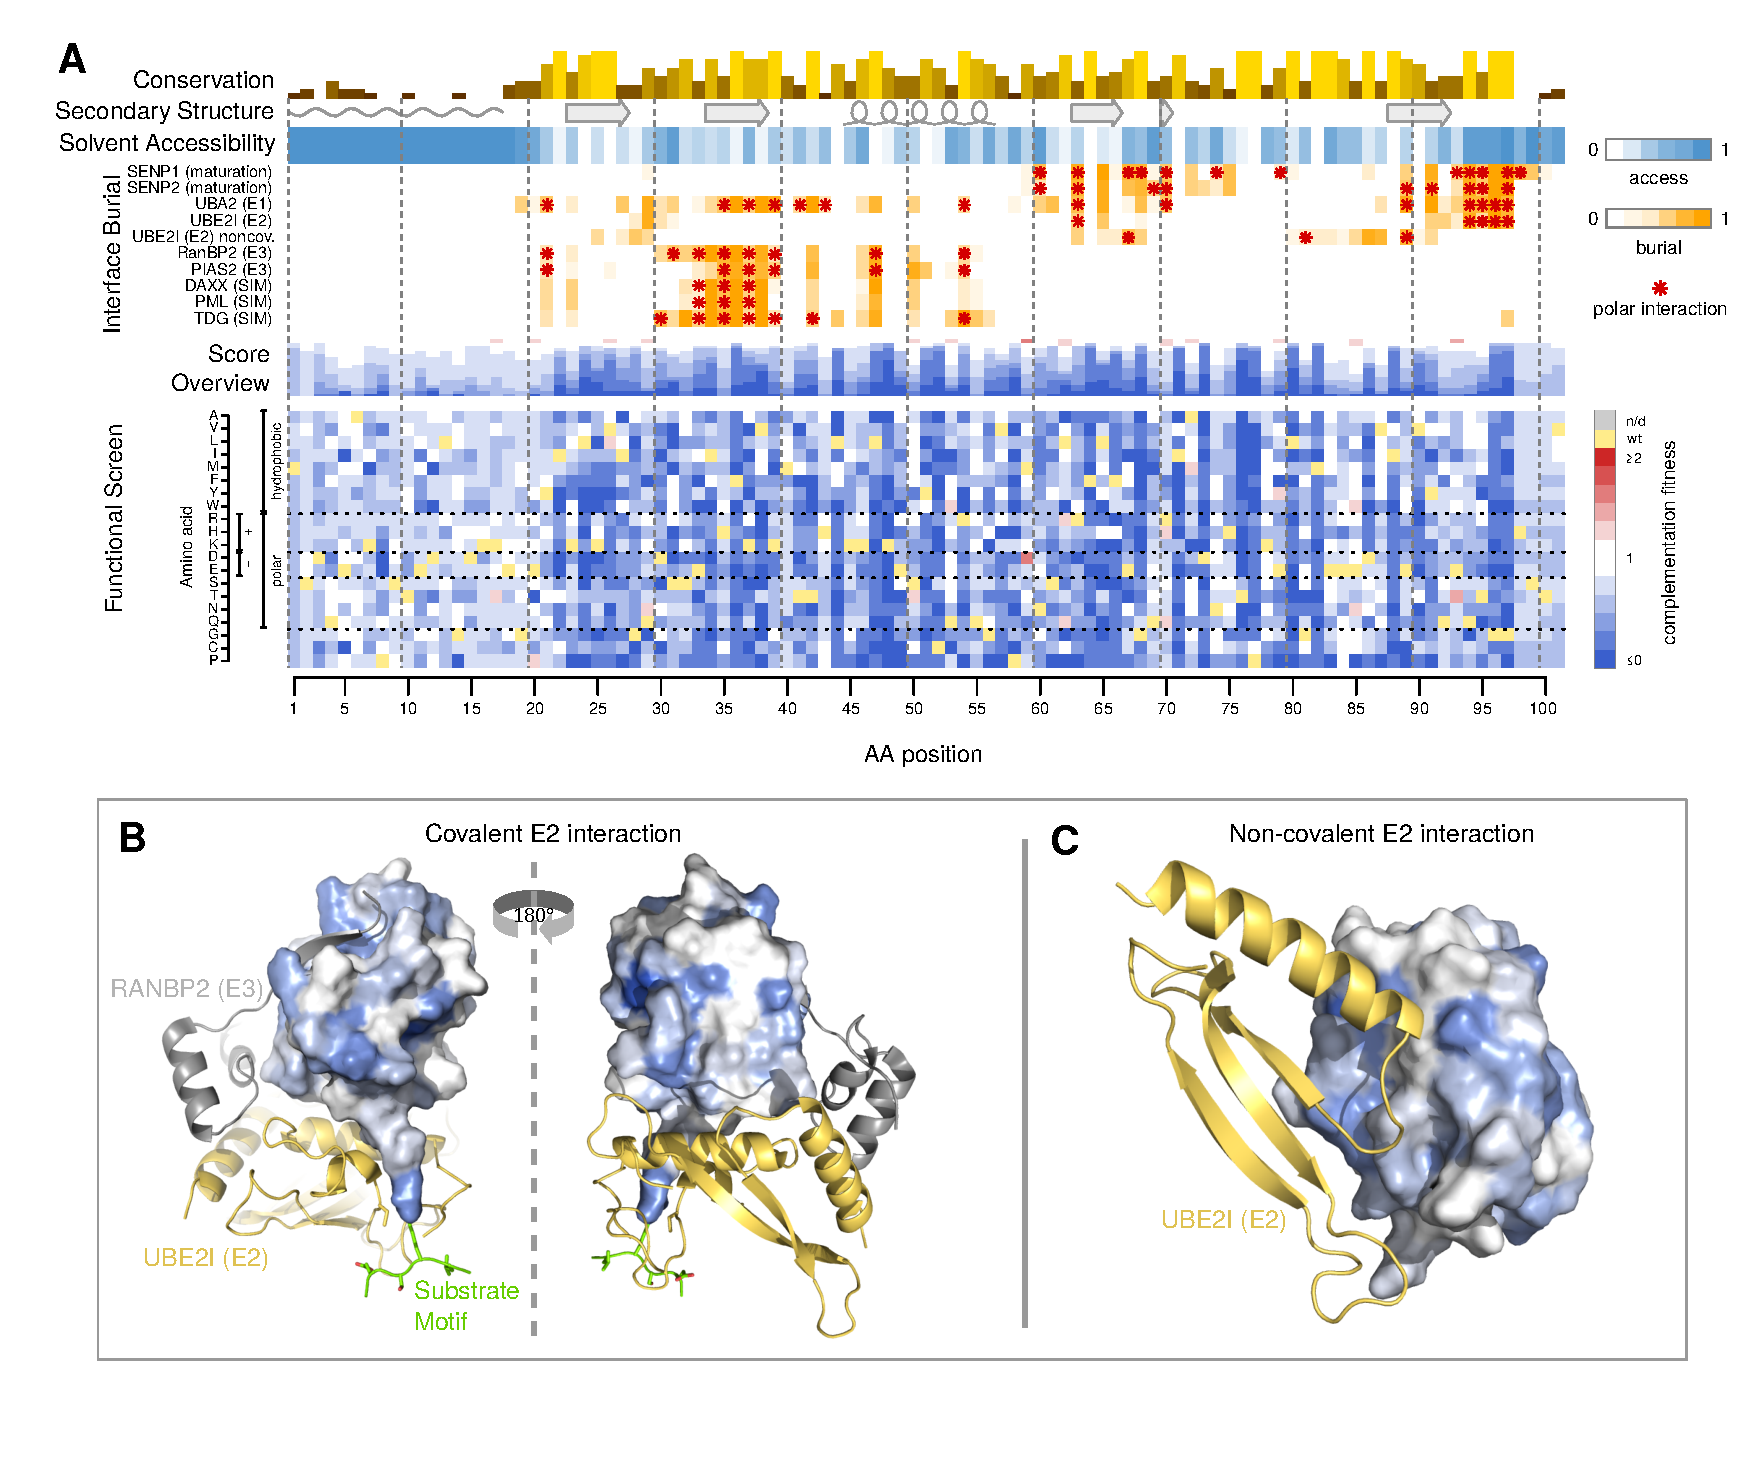
\includegraphics[width=\textwidth]{img/sumo-map.pdf}
	\caption{Functional map of SUMO1}
	\label{fig:sumo-map}
\end{figure}

The proximity and orientation of aspartate \#73 and lysine \#48 suggests that they are able to form a salt bridge with one another.  The importance of each residue according to the DMS map supports a model in which this salt bridge is important for SUMO folding and/or stability. Interestingly, substituting aspartate for methionine \#59, which points towards lysine \#48 from an angle similar to that of aspartate \#73, enhances the complementation fitness of SUMO1 beyond wild type levels.  This further underlines the potential importance of a polar interaction involving lysine \#48 (Figure~\ref{fig:saltbridge}).

\begin{figure}[h!]
	\centering
	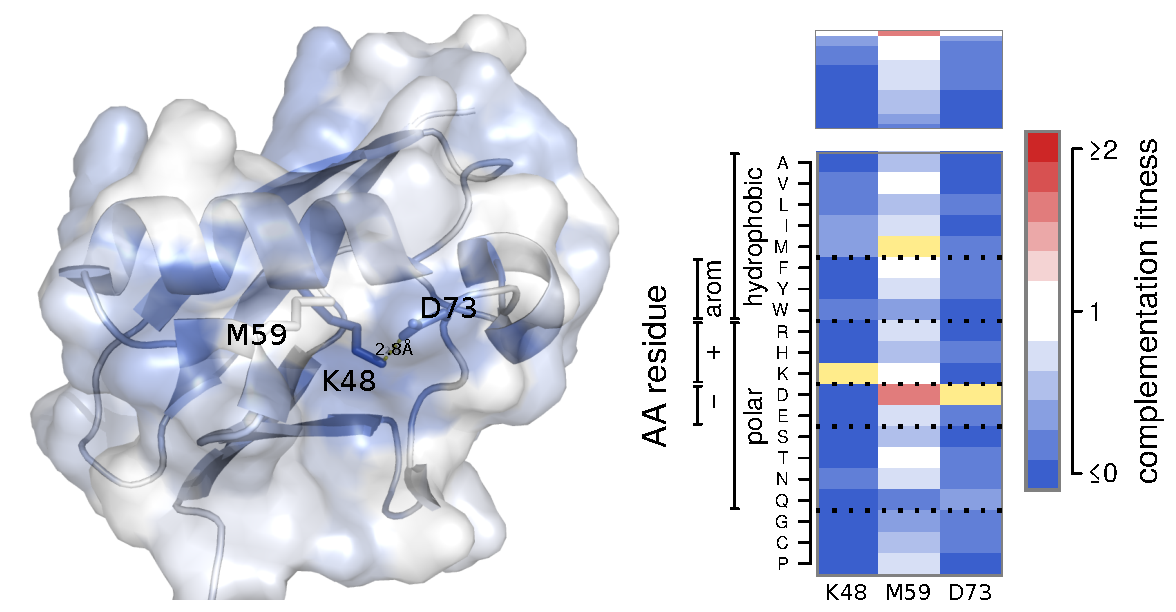
\includegraphics[width=\textwidth]{img/saltbridge.pdf}
	\caption{A salt bridge within SUMO1 between Asp73 and Lys38 appears important for stability. Met59Asp may increase stability even further.}
	\label{fig:saltbridge}
\end{figure}


% As was shown above for UBE2I, phylogenetic analysis of SUMO1 similarly showed that adaptive mutations with ability to complement yeast better than wild-type are likely deleterious in humans. We therefore transformed fitness scores so that such adaptive mutations are considered to be deleterious (see Methods).  However, because adaptive substitutions may provide interesting clues about differences between yeast and human cellular contexts, we provide both transformed (Figure 5) and untransformed versions of each map.




\subsection{Functional maps of three human disease genes}

Having established and evaluated our Deep Mutational Scanning framework on two members of the sumoylation pathway, we aimed to create maps for a diverse set of genes that have been associated with disease with varying degrees of confidence. While  heterozygous null mutations in SUMO1 have previously been associated with cleft palate, we wished to create maps that could be tested in the context of variant classification in terms of disease. Based on the availability of robust complementation assays, we applied DMS-TileSeq to the following protein targets: Thiamine Pyrophosphokinase 1 (TPK1), associated with vitamin B1 metabolism dysfunction; Neuronal Calcium Sensor 1 (NCS1), which has been implicated in autism based on a single \textit{de novo} mutation;  and CALM1, CALM2 and CALM3 associated with heart conditions long-QT syndrome and catecholaminergic polymorphic ventricular tachycardia. Although the three calmodulin genes differ in nucleotide sequence, each encodes the same polypeptide sequence. Thus, we performed a deep mutational scan only for CALM1, which enabled us to also map missense variant effects in CALM2 and CALM3. In each case, we used the TileSeq approach coupled with complementation to generate a map of missense variant functions. 


\begin{table}
	\centering
	\caption{Map quality comparison. RMSD: Root-Mean-Squared-Deviation in $10\times$ cross validation. $\max(\sigma_{\bar{x}})$: maximal standard error across non-imputed values in the map.\newline}
	\begin{tabular}{l p{.9in} p{.9in} p{1in} p{1in} p{1in}}
\textbf{Gene} & 
\textbf{Possible AA~changes} & 
\textbf{Achieved AA~changes} & 
\textbf{Imputation RMSD} & 
\textbf{Experimental $\max(\sigma_{\bar{x}})$} & 
\textbf{Regularized $\max(\sigma_{\bar{x}})$} \\ \hline\hline
\textbf{UBE2I} & 3021 & 2563 (85\%) & 0.24 & 0.36 & 0.25 \\
\textbf{SUMO1} & 1919 & 1700 (89\%) & 0.25 & 0.19 & 0.17 \\
\textbf{TPK1} & 4617 & 3181 (69\%) & 0.34 & 0.49 & 0.37 \\
\textbf{CALM1} & 2831 & 1813 (64\%) & 0.29 & 0.28 & 0.22 \\
\textbf{NCS1} & 3610 & 2542 (70\%) &  0.63 & 1.84 & 0.97
	\end{tabular}
	\label{tab:summary}
\end{table}



As was shown above for UBE2I, phylogenetic analysis of SUMO1 similarly showed that variants with ability to complement yeast better than wild-type are likely deleterious in humans. We therefore transformed fitness scores so that such adaptive mutations are considered to be deleterious \todo{expand on this}. The transformed disease gene maps can be seen in Figures \ref{fig:tpk1-map} and \ref{fig:calm+ncs1-maps}.  However, since adaptive substitutions may provide interesting clues about differences between yeast and human cellular contexts, we also provide untransformed versions of each map (see Appendix).

%%FIGURE: Map for TPK1/NCS1/CALM1


\subsubsection{A thiamine pyrophosphokinase map reflects a recessive phenotype}

Thiamine pyrophosphokinase (TPK1) is a protein that forms a dimer to perform its biochemical function. Its substrate, thiamine diphosphate, is bound within two active sites formed by the dimerization interface~\cite{timm_crystal_2001}. That is, each monomer contributes half of the residues making up each of the two active sites.  Each monomer in turn is made up of an N-terminal globular domain and a C-terminal $\beta$-sandwich domain (Figure~\ref{fig:tpk1_structure}A). The residues most sensitive to mutation in the protein make up the hydrophobic cores of the two domains: L21, V22, W36, G48, Y53, P65, G70, Y83, L108, I122, T124, and G127 for the N-terminal domain; and L161, G168, G199, L200, V227, V229, L236, and W237 for the C-terminal domain (Figure~\ref{fig:tpk1_structure}B). As might have been expected, mutation-sensitive residues include those closely involved in forming the active sites: D46, G70, D71, D73, D100, and K103 in the N-terminal half of the active site , contacting the diphosphate portion of the substrate (Figure~\ref{fig:tpk1_structure}C). In the C-terminal half of the active site, K203, L209, G212, L214, S216, T217, and N219 show similar sensitivity. Interestingly, the tryptophan residue at position 202 appears to be insensitive to mutation despite its close and extensive contact with the thiamine ligand. By contrast, a neighbouring lysine at position 201 is surprisingly sensitive suggesting potential importance in coordinating the ligand.  The remainder of the dimerization interface also features a number of sensitive residues, such as M136, G184, V188, G189 and G211. Finally, residues 1-12, which form a $\beta$-strand anchoring the N-terminal domain back to the C-terminal domain were also found to be sensitive.

\begin{landscape}
\begin{figure}[h!]
	\centering
	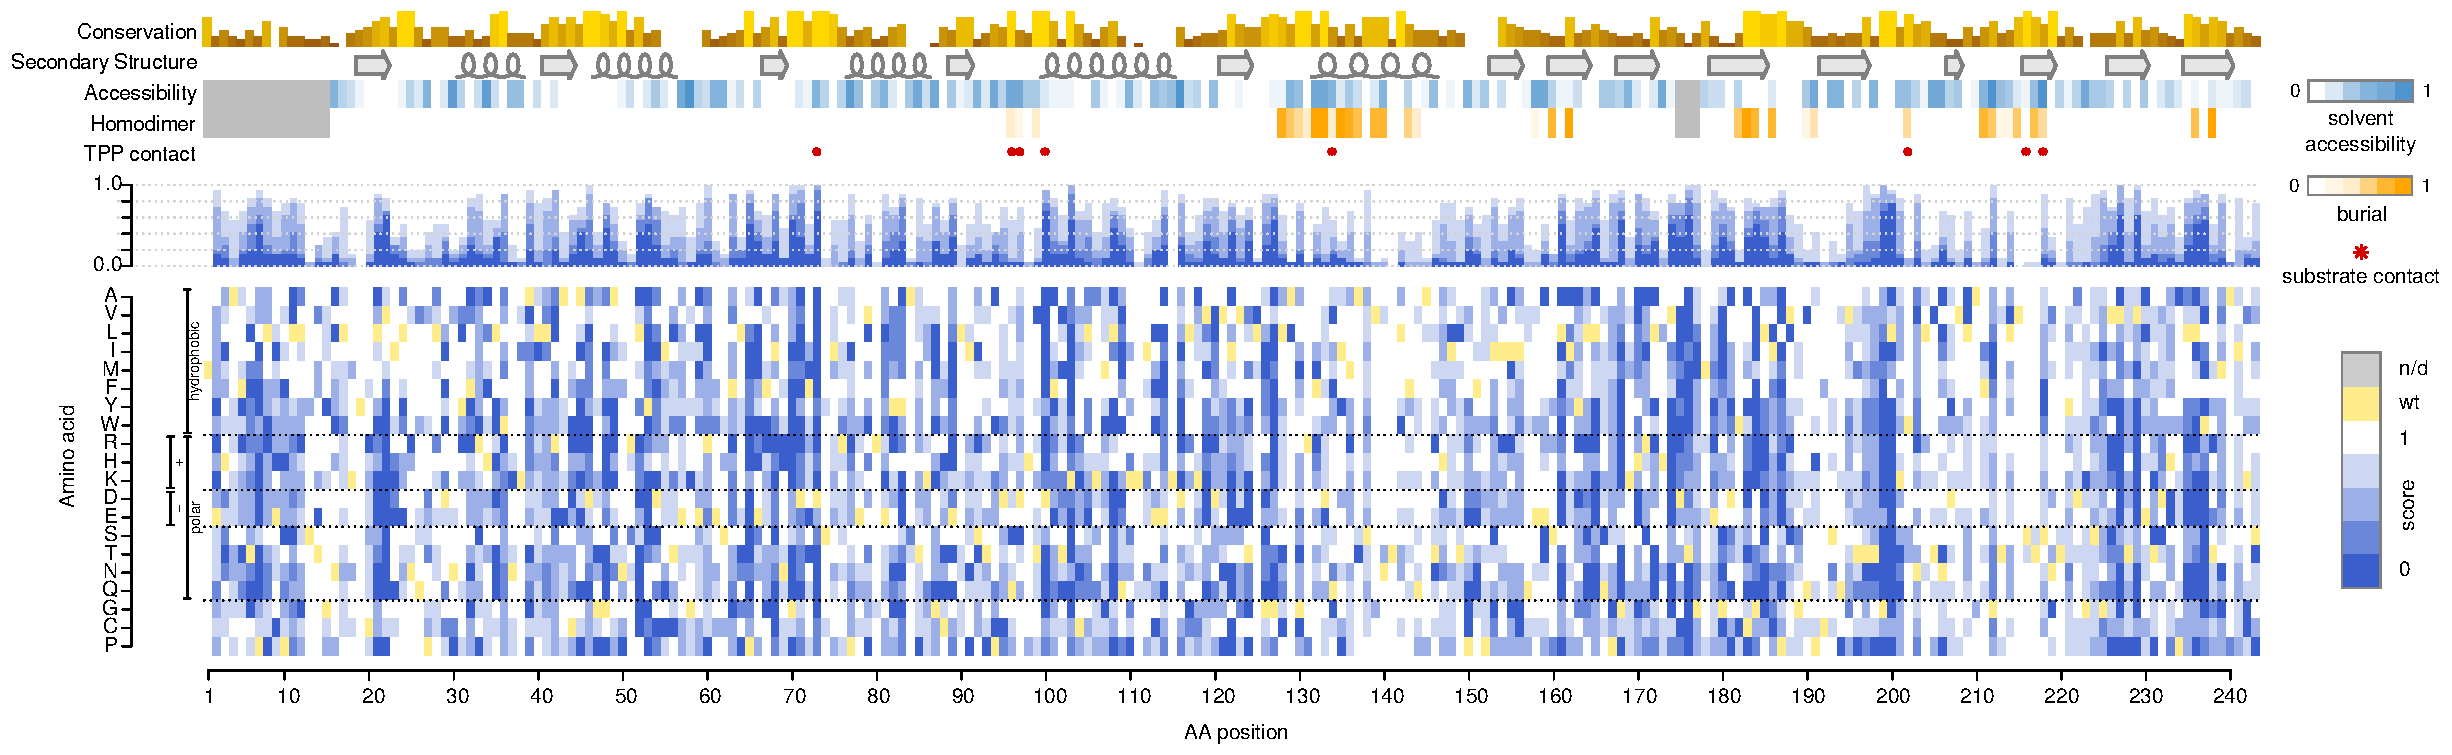
\includegraphics[width=9in]{img/tpk1-map.pdf}
	\caption{Functional map of Thiamine pyrophosphokinase 1 (TPK1). From top to bottom: Position-wise evolutionary conservation (AMAS); Secondary structure; Relative solvent accessibililty; Relative burial in homodimerization interface; Contacts with Thiamine diphosphate; Summary track showing the shares of amino acid changes resulting in varying degrees of fitness effects; Detailed heatmap showing individual amino acid change effects.}
	\label{fig:tpk1-map}
\end{figure}
\end{landscape}

\begin{figure}[h!]
	\centering
	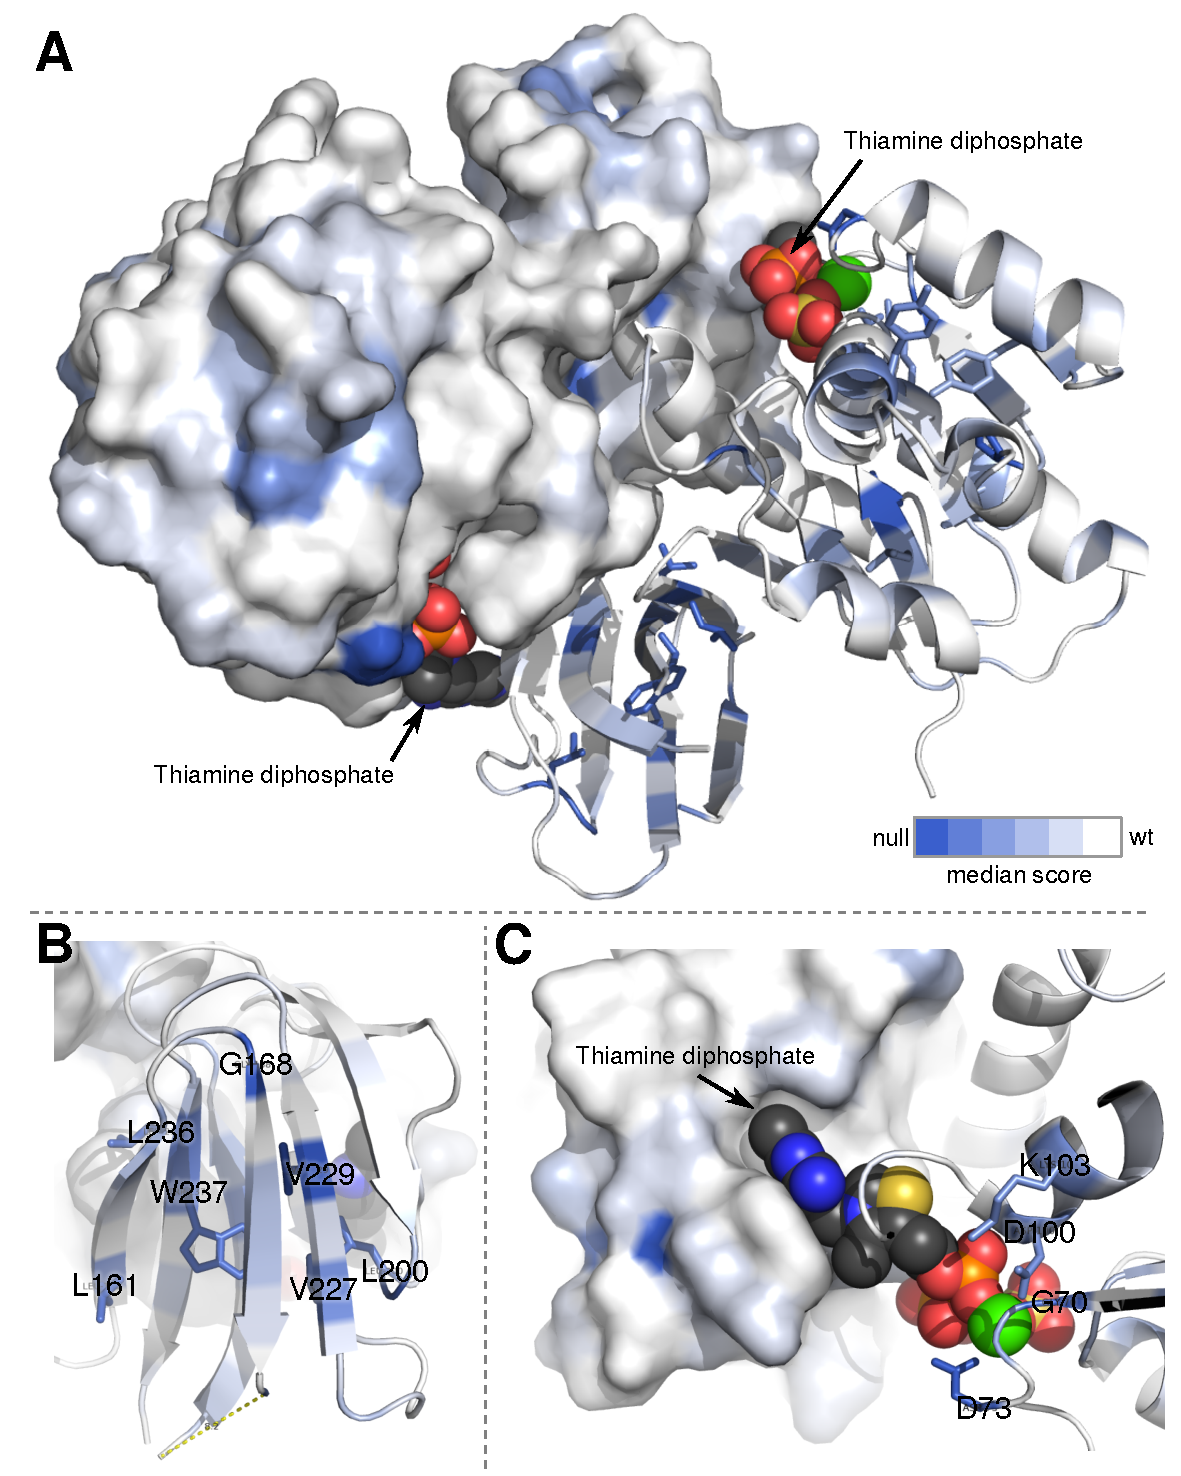
\includegraphics[width=.8\textwidth]{img/tpk1_structure.pdf}
	\caption{Thiamine pyrophosphokinase 1 colored by median complementation score. A) TPK1 homodimer structure showing one monomer as surface model, the other monomer as cartoon model. B) Hydrophobic residues facing the inside of the C-terminal $\beta$-sandwich domain are sensitive to mutation. C) Active site residues in contact with the substrate are sensitive to mutation. Structure data from \texttt{PDB:3S4Y}~\cite{timm_crystal_2001}}
	\label{fig:tpk1_structure}
\end{figure}


\subsubsection{The two calcium sensors NCS1 and Calmodulin show different profiles}

Calmodulin (CALM1/2/3) and the Neuronal Calcium Sensor protein (NCS1) are homologs (E-value $4 \cdot 10^{-5}$ when searched against the human proteome~\cite{altschul_basic_1990,the_uniprot_consortium_uniprot:_2015}) with 24\% sequence identity and 48.5\% similarity~\cite{rice_emboss:_2000}. However, they display different impact patterns despite their similar domain structure and similar molecular roles as calcium sensing proteins. Both are comprised of four Calcium-binding EF-hands, with NCS1 containing additional sequences upstream and downstream of the four hands. A comparison of previously published NMR structures reveals that the overall folds of the two proteins differ substantially~\cite{sarhan_crystallographic_2012,heidarsson_c-terminal_2012}. Calmodulin features a long central helix that separates two globular domains, called the N-lobe and the C-lobe, each comprised of two EF hands. A hydrophobic pocket serving as a binding interface for interacting proteins is nested within the C-terminal domain. NCS1, by contrast, forms a single shell-like shape, centered around a large hydrophobic crevice. This crevice acts as a binding interface for interacting proteins. Thus, the divergent DMS profiles we observed for CALM1/2/3 and NCS1 are consistent with these substantial structural differences.

The Neuronal Calcium Sensor NCS1 displays the greatest sensitivity to mutation within the N-terminal region containing the myristoylation site.  This myristoylation site is essential for anchoring NCS1 into the plasma membrane. One other residue that stands out is the tryptophan at position 30, which results in complete loss of function when replaced with any other amino acid. Like most other sensitive residues W30 is found among those contributing to the hydrophobic crevice acting as an interaction interface. Other cases include F55, F56, A104, M121, I152, and A182. An interesting observation can be made with respect to the two helices that separate the two N-terminal EF hands from the two C-terminal EF hands. A kink between the two helices brings them into an angle that allows a the globular shape of the overall protein to form. Without this kink it is conceivable that NCS1's fold would much more resemble that of Calmodulin. A glycine residue (G95) is likely responsible for forming that kink due to its helix breaking properties. This residue is also found to be quite sensitive to mutation.

Within Calmodulin, the regions most sensitive to mutation are: 1) the hydrophobic cores of the two globular domains; 2) interfacial residues for protein-protein interactions, and 3) a subset of the negatively charged residues in EF hands that contact Ca$^{2+}$ ions. Within the hydrophobic cores of the two lobes, five mutually interacting phenylalanine residues at positions 17, 69, 90, 93, and 142 stand out in particular, as all of them are found in the top 9 most sensitive residues on the map. Within the interaction interface, the residues D85, A89, F93, M100, L106, V109, L113, G114, L117, M125, V137, F142, M145, M146 are the most strongly sensitive to mutation. Regarding the four Calcium-binding EF-hand loops, we found it interesting that only a subset of the negatively-charged residues contacting Ca$^{2+}$ are even moderately sensitive. Within EF1, only D25 appears to be important, in EF2 only N61, in EF3 only D94 and D96, and in EF4 only D130 and D134. Overall, the EF3/4 in the C-lobe also appear to be more important than their N-lobe counterparts. This is in agreement with previous observations made by Sarhan and colleagues~\cite{sarhan_crystallographic_2012}, who described the C-lobe as the primary sensory mechanism. A number of unexplained sensitivities exist as well: Arginines at positions 54 and 91 show strong phenotypes despite extending from seemingly unused surfaces of the protein, offering the possibility that these residues are functionally relevant sites of interaction or modification.


\begin{landscape}
\begin{figure}[h!]
	\centering
	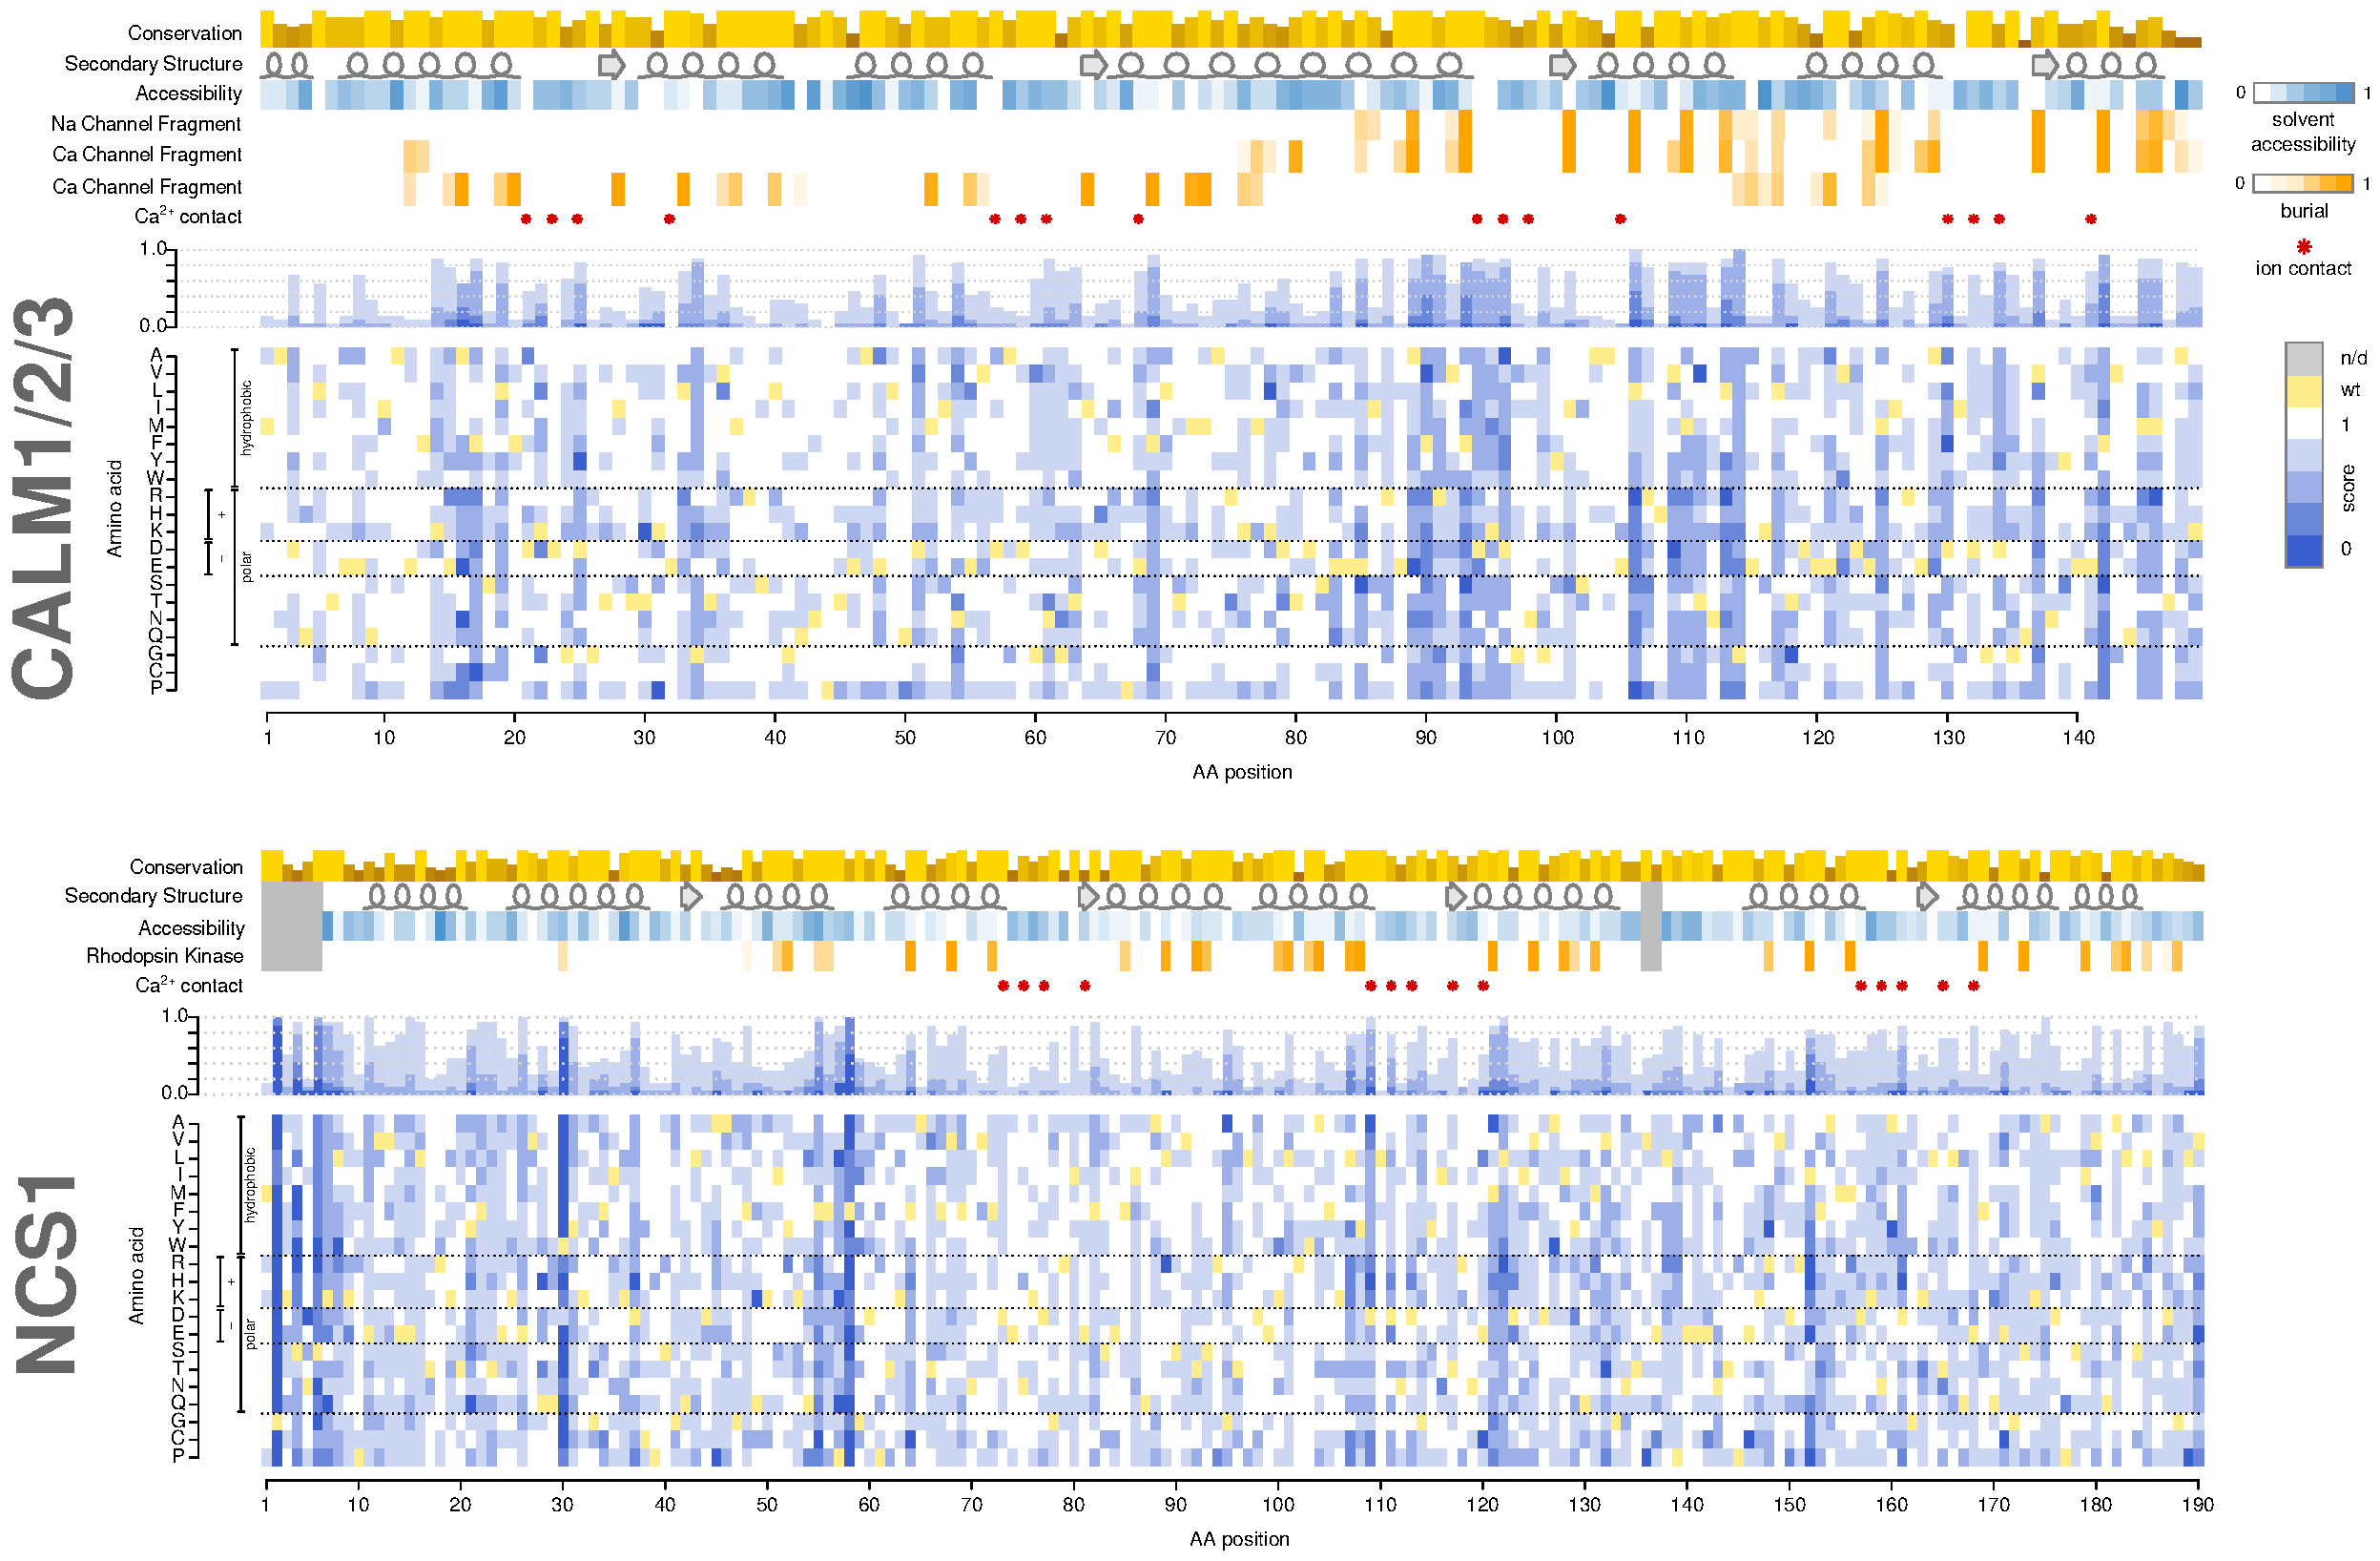
\includegraphics[width=9in]{img/calm+ncs1-maps.pdf}
	\caption{Functional map of Thiamine pyrophosphokinase 1 (TPK1). From top to bottom: Position-wise evolutionary conservation (AMAS); Secondary structure; Relative solvent accessibililty; Relative burial in homodimerization interface; Contacts with Thiamine diphosphate; Summary track showing the shares of amino acid changes resulting in varying degrees of fitness effects; Detailed heatmap showing individual amino acid change effects.}
	\label{fig:calm+ncs1-maps}
\end{figure}
\end{landscape}


\subsection{Functional maps recapitulate known disease cases}

To validate the utility of our maps in the context of human disease, we extracted known disease-associated variants from Clinvar~\cite{landrum_clinvar:_2016}, as well as rare and common polymorphisms observed independent of disease from GnomAD~\cite{lek_analysis_2016}, and somatic variants previously observed in tumors from COSMIC~\cite{forbes_cosmic:_2001}. 

For TPK1, a large number of very rare variants (minor allele frequency or $\text{MAF} < 10^{-6}$) is known from GnomAD. At first look, it appears the majority of these variants are shown to be deleterious (Figure~\ref{fig:tpk1_diploid}). This seems unlikely, given that Thiamine Metabolism Dysfunction Syndrome, reported to be caused by mutations in this gene, is a very severe disease to which patients succumb in childhood~\cite{mayr_thiamine_2011}., and that GnomAD attempts to filter out subjects with severe pediatric disease. However, the disease is also known to follow a recessive inheritance pattern, with only homozygous or compound heterozygous individuals being affected. We thus used phased sequence data from the 1000 Genomes Project~\cite{the_1000_genomes_project_consortium_global_2015} to determine the diploid genotypes in the TPK1 locus for all listed individuals and based our phenotype predictions based on the maximum fitness score of either allele. This improved prediction performance markedly, leading to complete separation between disease and non-disease genotypes. Both PROVEAN and PolyPhen-2 were also able to perfectly separate the two groups (Figure~\ref{fig:tpk1_diploid}B), so that additional compound heterozygotes with known disease status will be required to determine whether this DMS map is more useful than computational methods for classifying pathogenic TPK1 variants. 

\begin{figure}[h!]
	\centering
	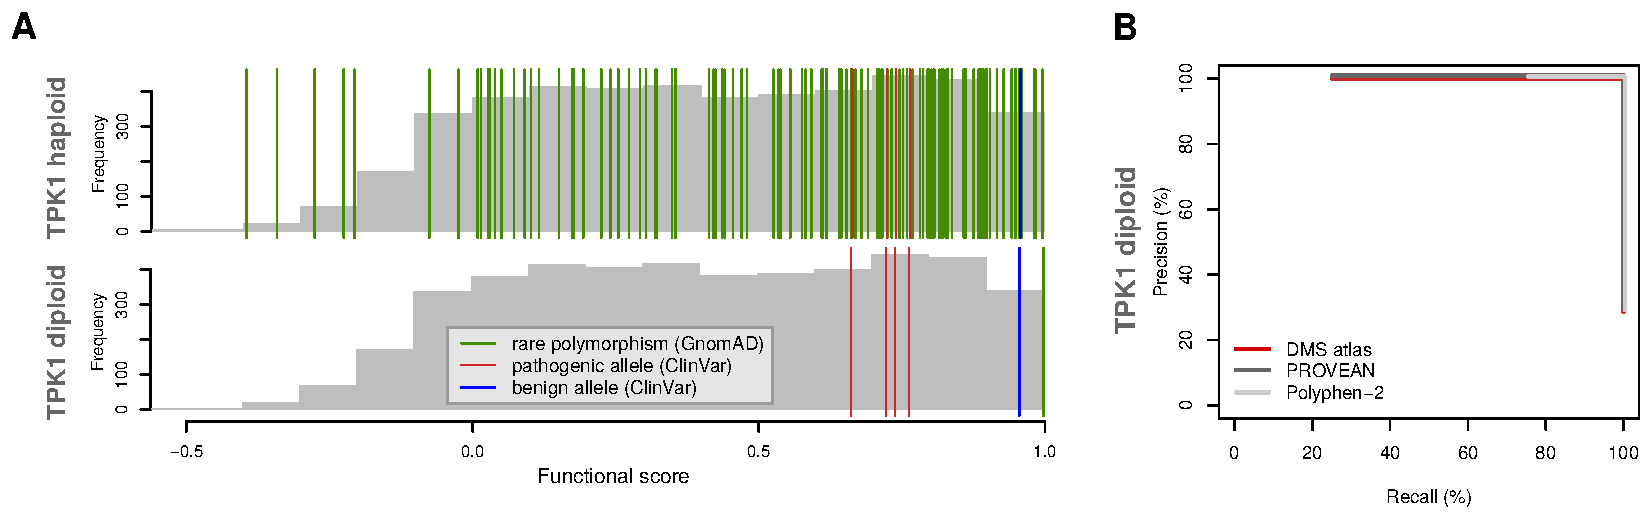
\includegraphics[width=\textwidth]{img/diploid.pdf}
	\caption{Variant classificationin TPK1. A) Distribution of functional scores for rare polymorphisms (GnomAD) (green) and pathogenic and benign variants (ClinVar) (red, blue) in TPK1 overlaid on a histogram of functional scores for all missense variant. Top panel: Haploid scores considering the phenotype based only on a single allele. Bottom panel: Diploid scores, considering the phenotype based on both alleles in each individual. B) Precision-Recall-Curve for disease variant classification using diploid scores from the atlas presented here, PROVEAN and PolyPhen-2, based on the data from (A).}
	\label{fig:tpk1_diploid}
\end{figure}


While NCS1 does not have any entries in ClinVar, a previous publication identified the variant R102Q as a \textit{de novo} variant in a single patient with autism spectrum disorder~\cite{handley_structural_2010}. While the variant did not affect overall protein folding and localization, the authors did observe that the dynamics of cytosol-membrane cycling were altered. Our complementation map did not show any functional impact for this variant.

As for NCS1, no disease-associated missense alleles are known for UBE2I and SUMO1 in ClinVar. However, a number of somatic mutations for all three genes have been observed in cancer according to COSMIC. While these can be expected to passenger mutations, one may still hypothesize that somatic variants are likely not subject to the same selection pressures as germline variants, as interference with developmental processes is not necessarily detrimental to a tumour. We thus tested whether germline polymorphisms in these three genes were enriched for being functional compared to their somatic counterparts in our maps. Indeed, we observed a significant difference between the two sets (Wilcoxon $P = 2.6 \cdot 10^{-5}$) (Figure~\ref{fig:calm_disease}C).

Finally, we examined our functional map of Calmodulin and found that it was able to distinguish disease variants from non-disease variants very well (Figure~\ref{fig:calm_disease}A). In contrast to TPK1, the Calmodulin map did not need to be corrected for diploid genotypes, as previously reported disease variants have been described as following a dominant inheritance pattern~\cite{crotti_calmodulin_2013}. A precision-recall (PRC) plot reveals a superior performance (AUC = 0.74) compared to PROVEAN (AUC = 0.47) and PolyPhen-2 (AUC = 0.47).  

\begin{figure}[h!]
	\centering
	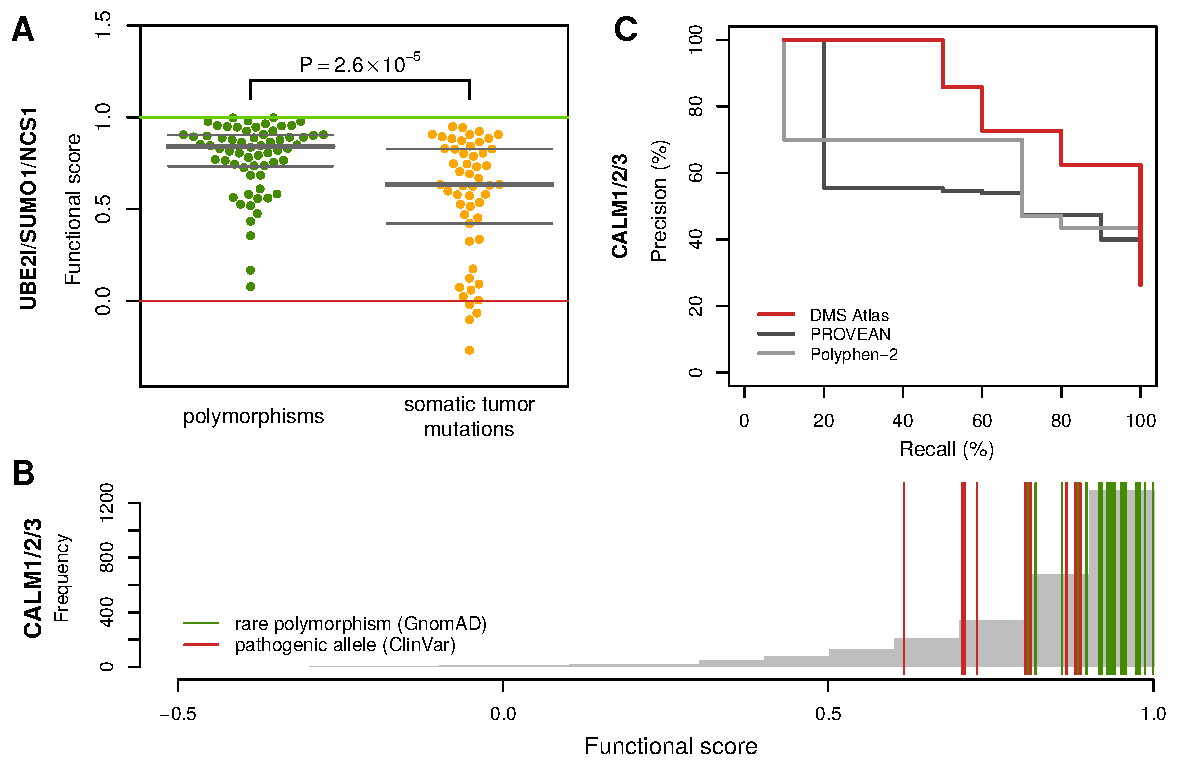
\includegraphics[width=\textwidth]{img/calm_disease.pdf}
	\caption{Detection of disease-associated variants. A) Distributions of functional scores for rare polymorphisms (GnomAD) (green) and for somatic in cancer (COSMIC) (gold) in UBE2I, SUMO1 and NCS1. B) Distribution of functional scores for rare polymorphisms (GnomAD) (green) and known pathogenic alleles (ClinVar) (red) in CALM1, CALM2 and CALM3, overlaid on a histogram of all missense variant scores (gray). C) Precision-Recall-Curves for classification of disease variants using the variant atlas presented here, PROVEAN and PolyPhen-2 in CALM1, CALM2 and CALM3 based on rare polymorphisms from GnomAD and pathogenic variants from ClinVar.}
	\label{fig:calm_disease}
\end{figure}


To further put our map to the test in a clinical scenario we inquired with Invitae, a company offering gene panel sequencing services for Long QT syndrome, including CALM1/2/3. In a blind test, we requested a list of Calmodulin variants they observed in patients but were unable to classify. After calibrating our map with respect to the above ClinVar and GnomAD datasets, we classified these 10 new variants (Table~\ref{tab:invitae}). Two were classified as damaging, six as benign, and two were too close to the threshold to be called either. In the next phase, Invitae revealed the associated patient cardiovascular phenotypes. Five out of the six patients with benign predictions were revealed to be healthy, while both patients with damaging predictions did show a positive phenotype. The two uncertain cases were revealed to be affected as well. A Mann-Whitney-U test showed these results to be statistically significant (P = 0.008).

\begin{table}[h!]
	\centering
	\caption{Re-classification attempt for variants of uncertain significance found in Invitae gene panel sequencing. MAF: Minor allele frequency in GnomAD, if known; sd/rmsd: standard error or RMSD of observation in map. imp/reg: imputed or degree of regularization; DMS score pre-regularization; DMS score post-regularization; DMS call: Classification according to DMS score; Indication: Type of sequencing panel ordered.\newline}
	%using a pdf file with individually colored cells
	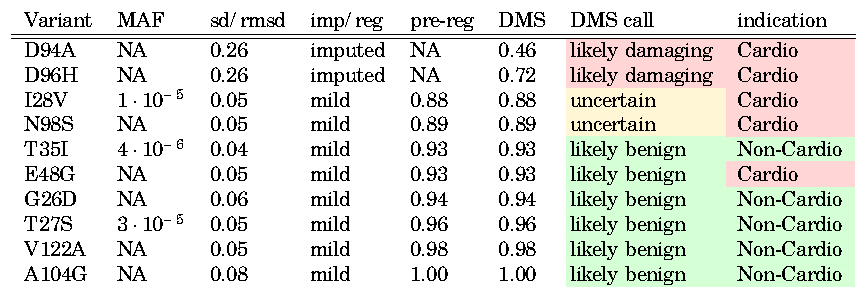
\includegraphics[width=\textwidth]{img/invitae.pdf}
	\label{tab:invitae}
\end{table}

% \begin{table}
% 	\centering
% 	\caption{}
% 	\begin{tabular}{l l l l l l l l}
% Variant & MAF & sd/rmsd & imp/reg & pre-reg & DMS & DMS call & indication \\ \hline\hline
% D94A & NA & 0.26 & imputed & NA & 0.46 & likely damaging & Cardio \\
% D96H & NA & 0.26 & imputed & NA & 0.72 & likely damaging & Cardio \\
% I28V & $1 \cdot 10^{-5}$ & 0.05 & mild & 0.88 & 0.88 & uncertain & Cardio \\
% N98S & NA & 0.05 & mild & 0.89 & 0.89 & uncertain & Cardio \\
% T35I & $4 \cdot 10^{-6}$ & 0.04 & mild & 0.93 & 0.93 & likely benign & Non-Cardio \\
% E48G & NA & 0.05 & mild & 0.93 & 0.93 & likely benign & Cardio \\
% G26D & NA & 0.06 & mild & 0.94 & 0.94 & likely benign & Non-Cardio \\
% T27S & $3 \cdot 10^{-5}$ & 0.05 & mild & 0.96 & 0.96 & likely benign & Non-Cardio \\
% V122A & NA & 0.05 & mild & 0.98 & 0.98 & likely benign & Non-Cardio \\
% A104G & NA & 0.08 & mild & 1.00 & 1.00 & likely benign & Non-Cardio
% 	\end{tabular}
% 	\label{tab:invitae}
% \end{table}



\section{Discussion}
\label{ch2discussion}

In total, this study has produced five maps with functional impacts for 15998 possible missense variants. The functional maps generated for sumoylation pathway members UBE2I and SUMO1 and disease-implicated genes NCS1, CALM1/2/3 and TPK1 using our framework were consistent with biochemical expectations while providing new hypotheses. DMS maps based on functional complementation were highly predictive of disease causing mutations, outperforming computational prediction methods such as PolyPhen-2 or PROVEAN5.  The imputation method we employed allows us to generate complete functional maps while maintaining the reliability on par with the experimental results. 

Given the prospect of personalized and precision medicine, genome sequencing is expected to become increasingly common in everyday medical practice. Current estimates suggest that every human carries an average of 200-300 rare mutations that have never before been seen in the clinic. This creates a need for fast, reliable interpretation of variant effects. Instead of generating clones and functionally testing variants of unknown significance after they are first observed, DMS technology offers to generate exhaustive maps of functional variation that enable interpretation immediately upon clinical presentation, even for rare and personal variation.

A key requirement for DMS mapping is an en masse functional assay that can be applied at the scale of 104-105 variant clones.  Among $\sim 4000$ disease genes, examination of four systematic screens and curated literature suggests that $\sim 5\%$ of human disease genes have a yeast complementation assay~\cite{5,33,34}. Complementation assays can also be carried out in human cells \todo{REF}, and \textit{en masse} transfection is achievable at the required scale \todo{REF}. Based on only three large-scale CRISPR studies~\cite{35-37}, cellular growth phenotypes have already been observed in at least one cell line for 29\% of human disease genes.  Beyond complementation, sub-functional assays, e.g. of protein interaction, can not only reveal variation that impacts the specifically assayed sub-function but also folding/stability mutations that ablate overall function. In a recent study, approximately two thirds of disease-causing variants were found to impact at least one protein interaction~\cite{38}. Although only a minority of human protein interactions have been mapped~\cite{39}, already 40\% of human genes have at least one interaction partner detectable by yeast two-hybrid assay in a recent screen~\cite{39}. Taking the union of available assays, we estimate that 57\% of known disease-associated genes already have an assay potentially amenable to DMS. Emerging protein interaction data and CRISPR screens suggests that the proportion of DMS-accessible disease genes will continue to rise. 

\section{Methods}

\subsection{DMS-TileSeq}
The DMS-TileSeq experiment for \gene{SUMO1}, \gene{TPK1}, \gene{NCS1}, and \gene{CALM1} was performed by Song Sun and Marta Verby as described in chapter~\cite{ch:data1}. The downstream sequencing data analysis, imputation and regularization was performed as described in chapter~\ref{ch:data1}.

\subsection{UBE2I interface analysis}
Co-crystal structure data for UBE2I was obtained from the PDB (Entries: \texttt{3UIP}~\cite{gareau_determinants_2012}; \texttt{4W5V}~\cite{reiter_characterization_2016}; \texttt{3KYD}~\cite{olsen_active_2010}; \texttt{2UYZ}~\cite{knipscheer_noncovalent_2007}; \texttt{4Y1L}~\cite{alontaga_rwd_2015}). A custom script was developed to obtain solvent accessibility using \texttt{GETAREA}~\cite{fraczkiewicz_exact_1998} for monomers and complexes, allowing for the calculation of relative burial of interfacial residues. Complementation fitness distributions for each interaction's interfacial residues were tallied and tested for statistically significant differences using Wilcoxon tests. Distributions were plotted using the R package `beeswarm'~\cite{eklund_bee_2016}

\subsection{Structure coloration} A custom script was developed to calculate median and maximum complementation fitness values for each residue and autogenerate coloration commands for OpenPyMol~\cite{schrodinger_pymol_2016}. 

\subsection{Complementation spotting assays} Complementation spotting assays were performed by Jennifer Knapp as described in chapter~\ref{ch:data1}. Image data was processed using PlateOrganizer and integrated and compared to the high-throughput results using custom scripts.

\subsection{Hyperactive mutation analysis}
\paragraph{Native amino acid analysis:} The UBE2I amino acid sequence was aligned to that of its orthologues in \species{S.~cerevisiae}, \species{D.~discoideum} and \species{D.~melanogaster} using \texttt{CLUSTAL}~\cite{russell_clustal_2014}. A custom script was used to extract inter-species amino acid changes and lookup the corresponding complementation fitness values in the UBE2I map. Distributions were plotted using the R package \texttt{beeswarm}~\cite{eklund_bee_2016}.

\paragraph{\textit{In vitro} sumoylation comparison} Images from \textit{in vitro} sumoylation assays performed for UBE2I variants by Bernier-Villamor~\etal~\cite{bernier-villamor_structural_2002} were scored by visual inspection while blinded to the underlying variant information. Scores were then represented as a heatmap and compared complementation scores from the UBE2I map.

\paragraph{Phylogenetic comparison of different models for hyperactive mutations}
The \texttt{phydms} software package~\cite{bloom_identification_2017} was used by Jesse Bloom to test three different models relating the effect of activity-enhancing mutations in SUMO1 and UBE2I to the actual evolutionary preference for that amino acid in a real biological context. Specifically, using the substitution models described in \cite{bloom_identification_2017}, three different ways of relating the evolutionary preference $\pi_{r,a}$ for amino-acid a at site $r$ to the fitness score $f_{r,a}$ for a given mutation were tested. 

In the first model, $$\pi_{r,a} = f_{r,a}.$$ 

In the second model, $$\pi_{r,a} = \min(f_{r,a}, f_{r,\text{wt}}),$$ where $f_{r,\text{wt}}$ is the fitness score for the wildtype amino-acid at site $r$. 

Finally, in the third model, $$\pi_{r,a} = \begin{cases} f_{r,a} &  \text{if}~ f_{r,a} \le f_{r,\text{wt}} \\ \frac{1}{f_{r,a}} & \text{otherwise} \end{cases}. $$ 

Each of these models were fit to the set of Ensemble homologues with at least 75\% sequence identity to the human protein. 

\subsection{Intragenic epistasis analysis} Genetic interactions were determined based on a previously described multiplicative model~\cite{phillips_language_1998,onge_systematic_2007}, that expects double mutant fitness to conform to the product of single mutant fitness effects in the absence of interaction between the two. Under this model, the strength of genetic interaction is defined as $$\varepsilon_{ij} = f_i \cdot f_j - f_{ij},$$ where $f_i$ and $f_j$ represent single mutant fitness and $f_{ij}$ represents double mutant fitness scores. To test for deviation from this model, all cases where double mutant and both corresponding single mutants were known in the data were extracted. The standard deviation for the expected double mutant fitness $f_i \cdot f_j$ was estimated using
$$ \mathbb{V}(XY) = \mathbb{E}(X^2Y^2)-(\mathbb{E}(XY))^2=\mathbb{V}(X)\mathbb{V}(Y) + \mathbb{V}(X)(\mathbb{E}(Y))^2+\mathbb{V}(Y)(\mathbb{E}(X))^2 $$ 
%$$ \bar{\sigma}_{i,j} = \sqrt{\sigma_i^2 \cdot \sigma_j^2 + \sigma_i^2 \cdot \mu_j^2 + \sigma_j^2 \cdot \mu_i^2},$$ 
%where $\sigma_i , \sigma_j$ are the standard deviations and $\mu_i , \mu_j$ are the means of the single mutant fitness measurements.
Using these estimates, Student t-tests were performed between the measured and expected double mutant fitnesses and corrected for multiple hypothesis testing using the  Benjamini-Hochberg~\cite{benjamini_controlling_1995} method at a 5\% FDR threshold.

To detect potential direct compensatory relationships, the genetic interactions were compared with physical distance in the protein's 3D structure. The euclidean distance between the C$_\alpha$ atoms in of each pair of residues was calculated using a custom script using structural data from \texttt{PDB:3UIP}~\cite{gareau_determinants_2012}.



\subsection{Structural analysis of disease gene maps}
Co-crystal and NMR structure data for SUMO1, TPK1, NCS1 and CALM1 was obtained from the PDB (Entries: \todo{Check Desktop HD for SUMO files that were used}). Structures were colorized using the same method described above for UBE2I.

\subsection{Disease variant analysis}
Missense variant tables for \gene{UBE2I}, \gene{SUMO1}, \gene{TPK1}, \gene{NCS1}, \gene{CALM1}, \gene{CALM2} and \gene{CALM3} were integrated ClinVar, COSMIC, and GnomAD and compared with complementation scores. To calculate diploid scores for TPK1, phased variant call files (VCF) for the TPK1 gene obtained from the 1000 genomes project database to identify homozygous, heterozygous and compound heterozygous cases for all present variants using a custom script. For each case, the diploid score was calculated as $s_\text{diploid} = \max(s_1,s_2)$, where $s_1$ and $s_2$ are the variant scores for the paternal and maternal allele.


\chapter{Conclusion}

\section{Summary}

Here we have presented a complete framework for the construction of comprehensive, high-fidelity functional maps. We have demonstrated two versions of this framework: DMS-BarSeq, a barcode-based approach that allows for high-confidence measurement of individual clones including double- and higher-order multi-mutants; and DMS-TileSeq, a fast and efficient framework that generalizes fitness effects over many different clones sharing variants of interest. Both versions use a new mutagenesis protocol, POPCode, which thanks to its accompanying webtool makes it easer than before to generate variant libraries covering the complete space of amino acid changes. At its core, the framework relies on a functional complementation assay in yeast, which can measure the overall effect of variants on protein function and has been shown to be highly predictive of variant pathogenicity in humans, outperforming common \textit{in silico} methods, despite the $\sim$ 1 billion year divergence between the two organisms. 
The DMS analysis software developed here introduces novel advances to deep mutational scanning: (i) The degree of confidence behind each measurement is carefully assessed and recorded in order to help variant classification; and (ii) variants that were missing in the complementation library or measured with low confidence were supplemented using a RandomForest-based machine learning method, whose predictions were found to be surprisingly reliable. 

We have evaluated the technical features of the framework on the two sumoylation pathway members UBE2I and SUMO1. We found that the functional maps generated with our method were able to successfully recapitulate known features of the proteins' biology and biochemistry and even hint at novel features that warrant further investigation. We found a large number genetic interactions between variants in UBE2I, some of which may be due to direct compensatory relationships of amino acid replacements. Most interactions however were found to involve residue pairs separated by larger physical distances.

Having validated the framework, we demonstrated its power to detect pathogenic variants in the disease genes \gene{TPK1}, \gene{NCS1}, \gene{CALM1}, \gene{CALM2} and \gene{CALM3}.  
We found that our Calmodulin map excelled at distinguishing disease-associated variants from benign polymorphisms and greatly outperformed the common prediction algorithms PolyPhen-2 and PROVEAN. We subsequently applied our functional map for \gene{CALM1}, \gene{CALM2} and \gene{CALM3} to classify VUS observed in patients during gene panel sequencing and found our predictions to be closely matching patient indications.

\subsubsection{Limitations of the DMS framework}
Despite these successes, there are a number of limitations the current form of our DMS framework. A fairly simple problem is the current restriction to scan relatively short genes. This is due to three reasons: (1) Longer genes would require a re-formulation of the mutagenesis protocol, as the number of mutations introduced per clone can be expected to increase linearly with gene length. This would need to be addressed by varying the concentration of mutant oligos in the amplification step. This could be tested systematically for templates of different lengths to determine the exact relationship between the factors involved. The results can then be added to the POPCode oligo design software to automatically report the most suitable protocol for each case to the experimenter.
(2) Variant clone pools for longer genes must be kept in larger volumes at all times to avoid bottlenecking the complexity of the pools.
(3) Finally, larger libraries also require more sequencing reads to cover all variants at adequate depth. Thus they either require the use of higher-throughput equipment or would have to be processed in batches. 
A relatively easy solution to all three problems would be subdivide longer genes into sections that would be scanned separately from each other, although this would be more time consuming and costly.

A more difficult problem is that currently, the number of genes amenable to functional complementation in yeast is very limited. Song Sun and other members of the Roth lab have previously determined that only 60 human disease genes can currently been examined using this assay~\cite{sun_extended_2016}. In addition, we found that some of these genes suffer from mapping quality issues. We observed this in the \gene{NCS1} map, which was of lower quality compared to other genes due to its relatively weak wildtype complementation fitness resulting in a less favourable signal-to-noise ratio. However it is possible that these assays might be improved by using different yeast strains with different backgrounds or by using different growth conditions.
Moreover, as mentioned in section~\ref{ch2discussion} of the previous chapter, we have determined that 57\% of disase genes could be assayed using DMS variants based on Y2H or human cell lines instead, as will be discussed in further detail in the next section.


\section{Outlook}

\subsection{Using DMS data in a clinical context}
%DMS in clinical contexts
As introduced in chapter 1, a major motivation factor behind the development of our framework is to address the growing problem of variants of uncertain significance observed in the clinic. While our results show that functional maps as produced by our framework can be helpful in the effort of VUS reclassification, a single line of evidence is not usually sufficient. Even though the ACMG considers functional assays among the strongest classification criteria, they require at least one additional criterium of moderate strength, such as enrichment in cases over controls, or negligible allele frequency in the general population~\cite{richards_standards_2015}. While most of the information informing the required criteria cannot be generated \textit{en masse}, other information, such as allele frequencies in the general population are available from the 1000 genomes project~\cite{the_1000_genomes_project_consortium_global_2015} and the genome and exome aggregation database (GnomAD)~\cite{lek_analysis_2016}. Thus an important goal for the future would be the construction of a public database with an underlying automatic data integration and classification system, that obtains information from available sources and automatically applies the ACMG's recommended decision-making process towards variant classification. Classification results should be presented transparently, revealing the individual underlying evidence, confidence levels and reasoning structure. 

However, the commitment towards the construction of a resource is only warranted if its primary source of information, functional maps generated using Deep Mutational Scanning can continue to be provided. The Roth Lab is planning to continue building functional maps of disease genes and to expand the list of genes amenable to deep mutational scanning. A shortlist of $\sim$100 genes is planned to be addressed in the coming years. However, this undertaking is a costly one. Per 500 amino acid positions scanned, approximately \$5500 need to be spent on consumables, primarily for sequencing and oligos for POPCode mutagenesis. Assuming 6 genes being scanned in parallel, approximately 45 full-time employee hours need to be invested per gene. Ultimately, this undertaking cannot be stemmed by one lab alone and will require outreach to other groups. As shown in chapter~1 section~\ref{dmsIntro} a fair amount of groups are already performing deep mutational scans, who may be interested in collaboration. As a first step, the Roth and Fowler labs are already planning on collaborating with respect to mapping a number of heart-disease associated genes.

\subsection{Adaptation and extentions to DMS technology}
\subsubsection{DMS in human cell lines}
As mentioned above, an important future direction is the adaptation of the deep mutational scanning framework toward directly using human cell lines in the competition assays. Recent genome-wide CRISPR screens have revealed a sizable number of genes with growth phenotypes in different human cell lines~\ref{?}~todo{REF}. While a number of DMS efforts have already been performed using human cells~\cite{forsyth_deep_2013,wagenaar_resistance_2014,doud_site-specific_2015,majithia_prospective_2016}, the underlying assays were not generalizable, for example, the most recent effort by Majithia and colleagues~\cite{majithia_prospective_2016} for PPAR$\gamma$ was only possible due to the fortuitous circumstances of having found a surface marker whose expression level directly reflects PPARG$\gamma$ activity. 
Atina Cote in the Roth Lab is currently working on establishing a generalizable growth-based assay using CRISPR in human cell lines. 
%previous work: PPARG
%atina's CRISPR lines
%fowler's stability assay

\subsubsection{Screening of other functional elements}
Another important future direction is to expand the capability of Deep Mutational Scanning to enable the assaying of variants outside of protein-coding regions of the genome. However, since the space of the human genome is simply too large to be tested in its entirety the logical choice is to concentrate on elements most likely to be functionally relevent, such as splice sites, promoters, or transcription factor binding sites.
Hanane Ennajdaoui in the Roth Lab is currently working on adapting our DMS framework to scan intron boundaries.
%spliceDMS

\subsection{Other uses of DMS functional map data}

\subsubsection{Screening for viral suppressors}
%UBE2I as viral target

\subsubsection{Advances in computational prediction of disease variants}
%extrapolation
%  -> FUNSUM

\subsubsection{Functional classification of amino acid positions}

%clustering of AA positions
% -> functional classes


\begin{appendices}
\chapter{Variant maps with hypercomplementation}
\label{apdx:maps}
As was shown in chapter 3 section~\ref{sec:hypercomp}, phylogenetic analysis of \gene{UBE2I} and \gene{SUMO1} both showed that variants with ability to complement yeast better than wild-type are likely deleterious in humans. Thus, fitness scores were transformed so that such hypercomplementing mutations are considered to be deleterious. However, since hypercomplementing substitutions may provide interesting clues about differences between yeast and human cellular contexts, the untransformed versions the maps are provided below.

\begin{landscape}
\begin{figure}[h]
	\centering
	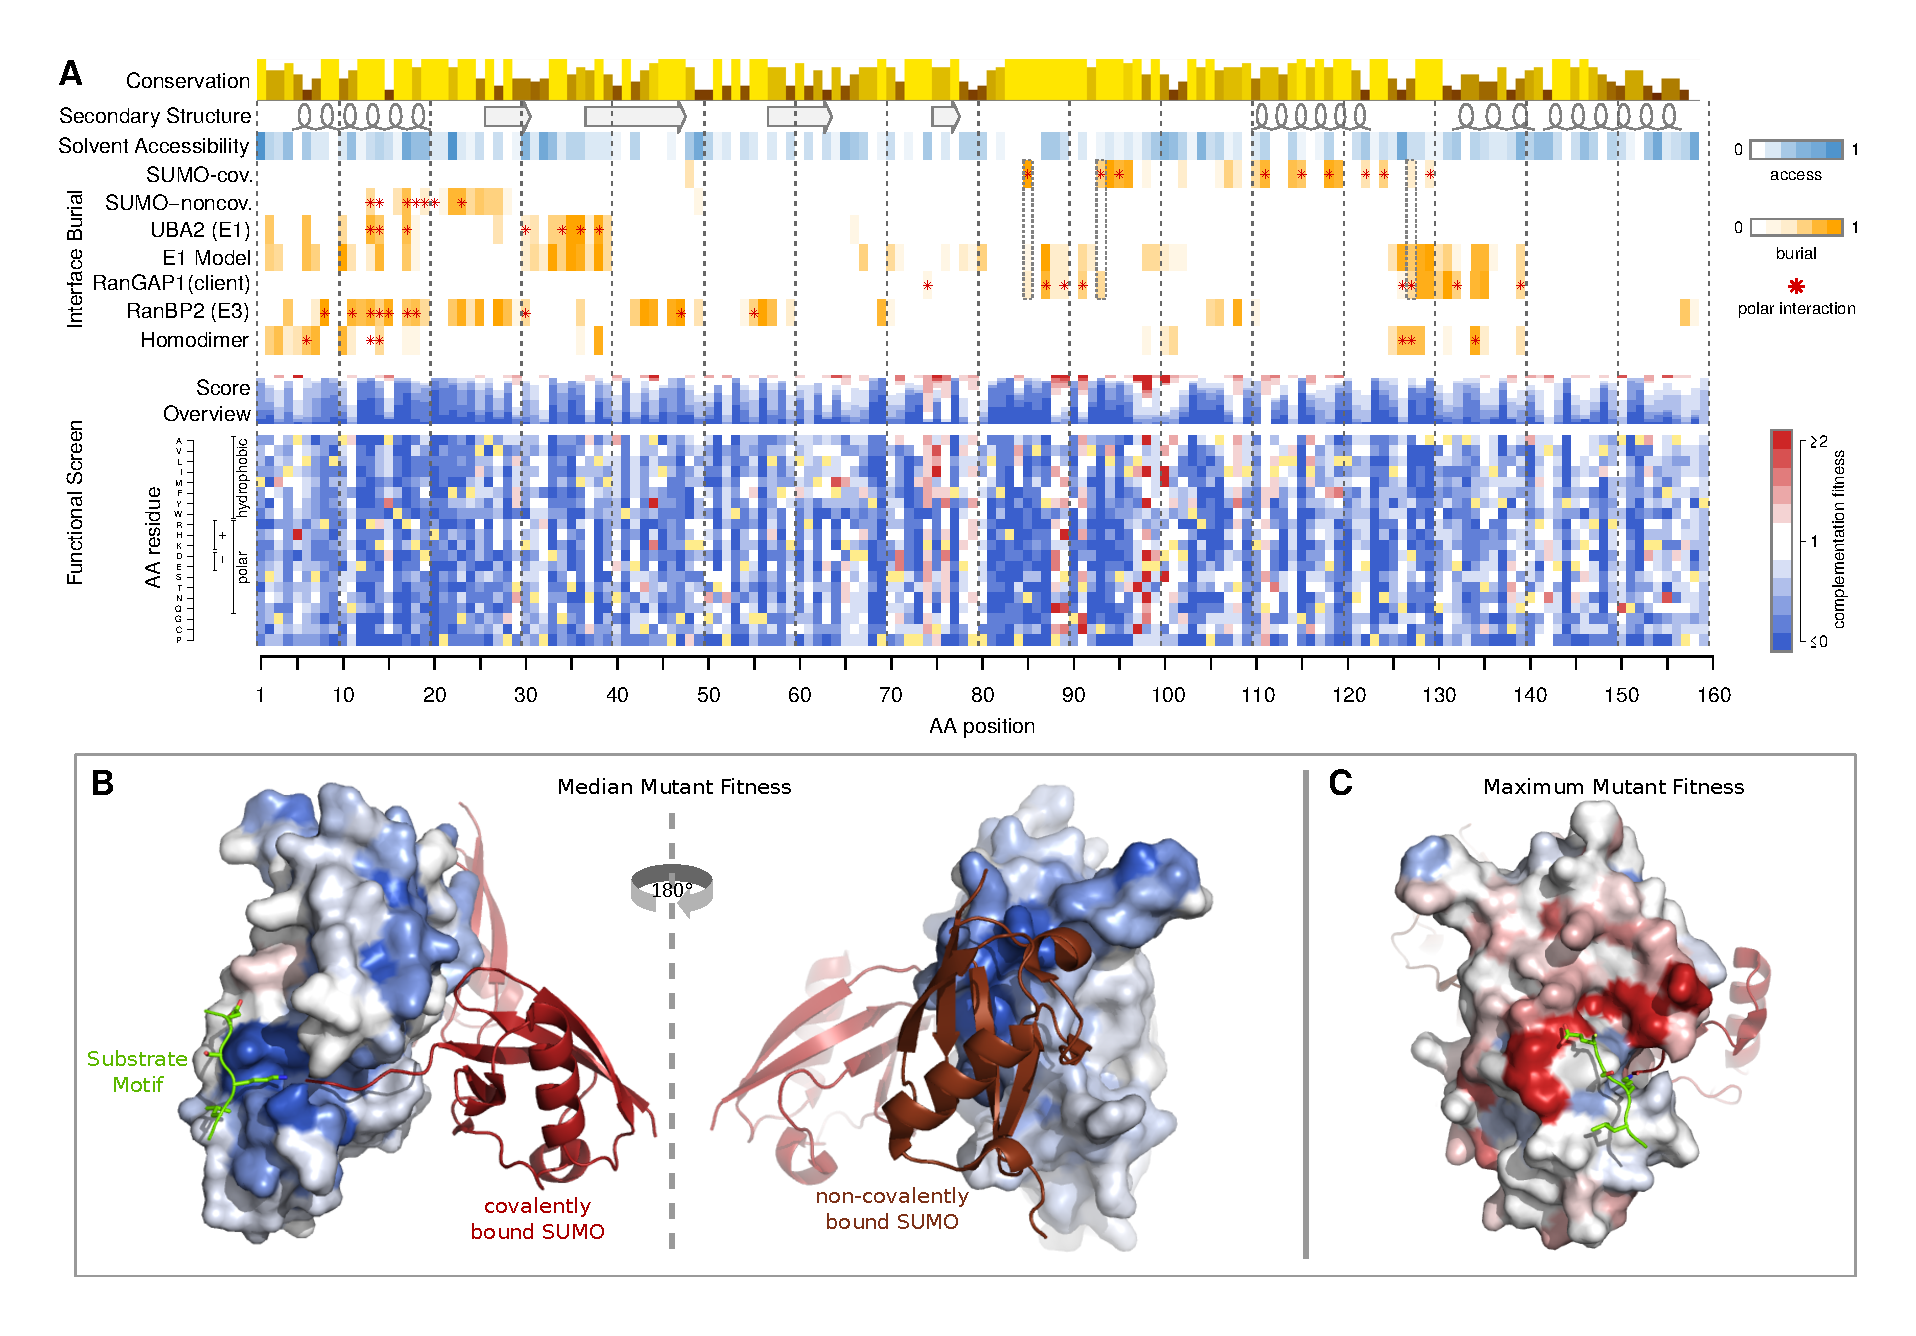
\includegraphics[width=9in]{img/ube2i_map.pdf}
	\caption{Functional map of UBE2I. From top to bottom: Position-wise evolutionary conservation (AMAS); Secondary structure; Relative solvent accessibility; Relative burial in protein-protein interaction interfaces with covalently bound SUMO, non-covalently bound SUMO, the SUMO E1 complex at two different stages of activation, the sumoylation substrate RanGAP1, the E3 RanBP2, and the UBE2I homodimer; A summary track showing the relative number of amino acid changes resulting in different fitness effects; and finally the individual amino acid change effects sorted by physicochemical groups.}
\end{figure}
\end{landscape}


\begin{landscape}
\begin{figure}[h]
	\centering
	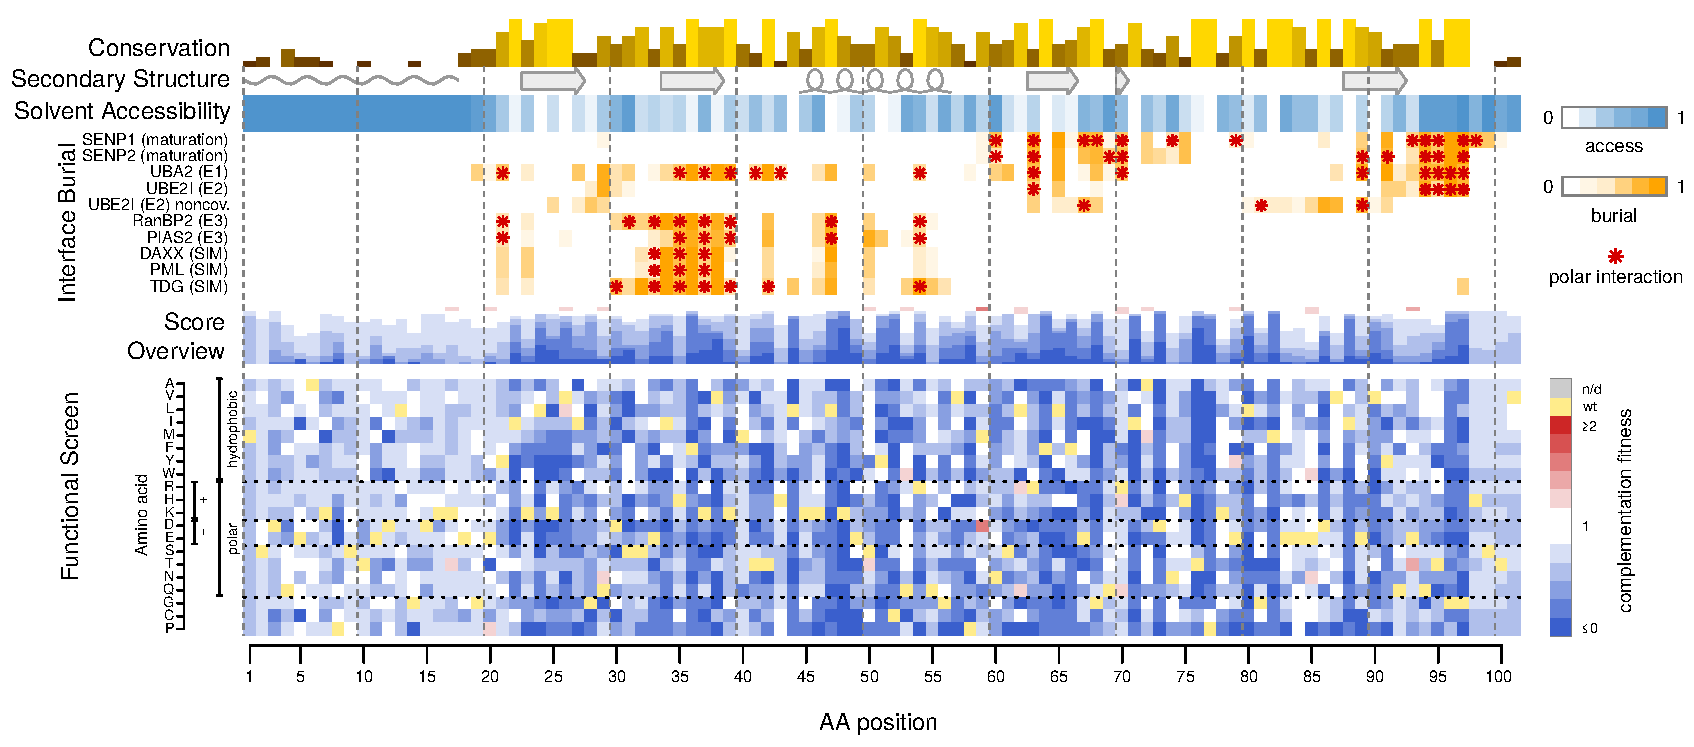
\includegraphics[width=9in]{img/sumo1_map_noflip.pdf}
	\caption{Functional map of SUMO1. From top to bottom: Position-wise evolutionary conservation (AMAS); Secondary structure; Relative solvent accessibility; Relative burial in protein-protein interaction interfaces with SENP proteases, E1 complex, covalent and noncovalent E2 binding, E3s and three different SIM motifs; A summary track showing the relative number of amino acid changes resulting in different fitness effects; and finally the individual amino acid change effects sorted by physicochemical groups.}
\end{figure}
\end{landscape}


\begin{landscape}
\begin{figure}[h]
	\centering
	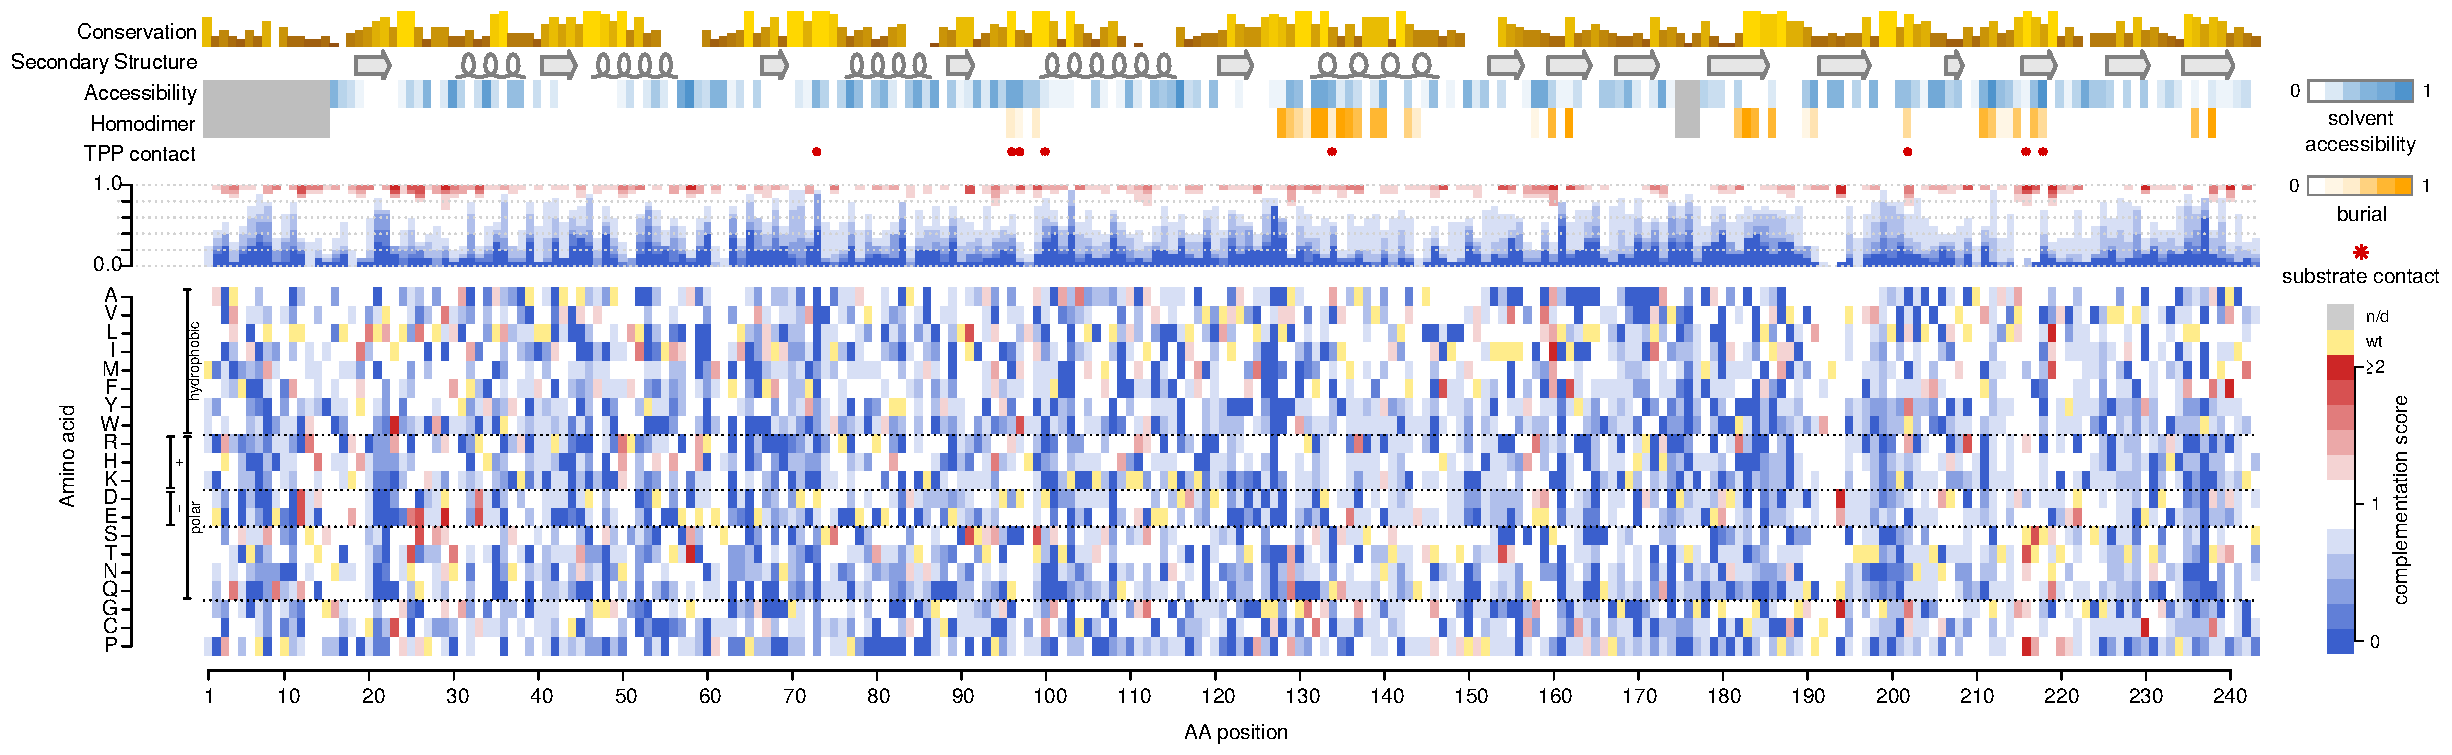
\includegraphics[width=9in]{img/tpk1_map_noflip.pdf}
	\caption{Functional map of TPK1. From top to bottom: Position-wise evolutionary conservation (AMAS); Secondary structure; Relative solvent accessibility; Relative burial in homodimerization interfaces; Positions contacting the Thiamine pyrophosphate (TPP) molecule; A summary track showing the relative number of amino acid changes resulting in different fitness effects; and finally the individual amino acid change effects sorted by physicochemical groups.}
\end{figure}
\end{landscape}


\begin{landscape}
\begin{figure}[h]
	\centering
	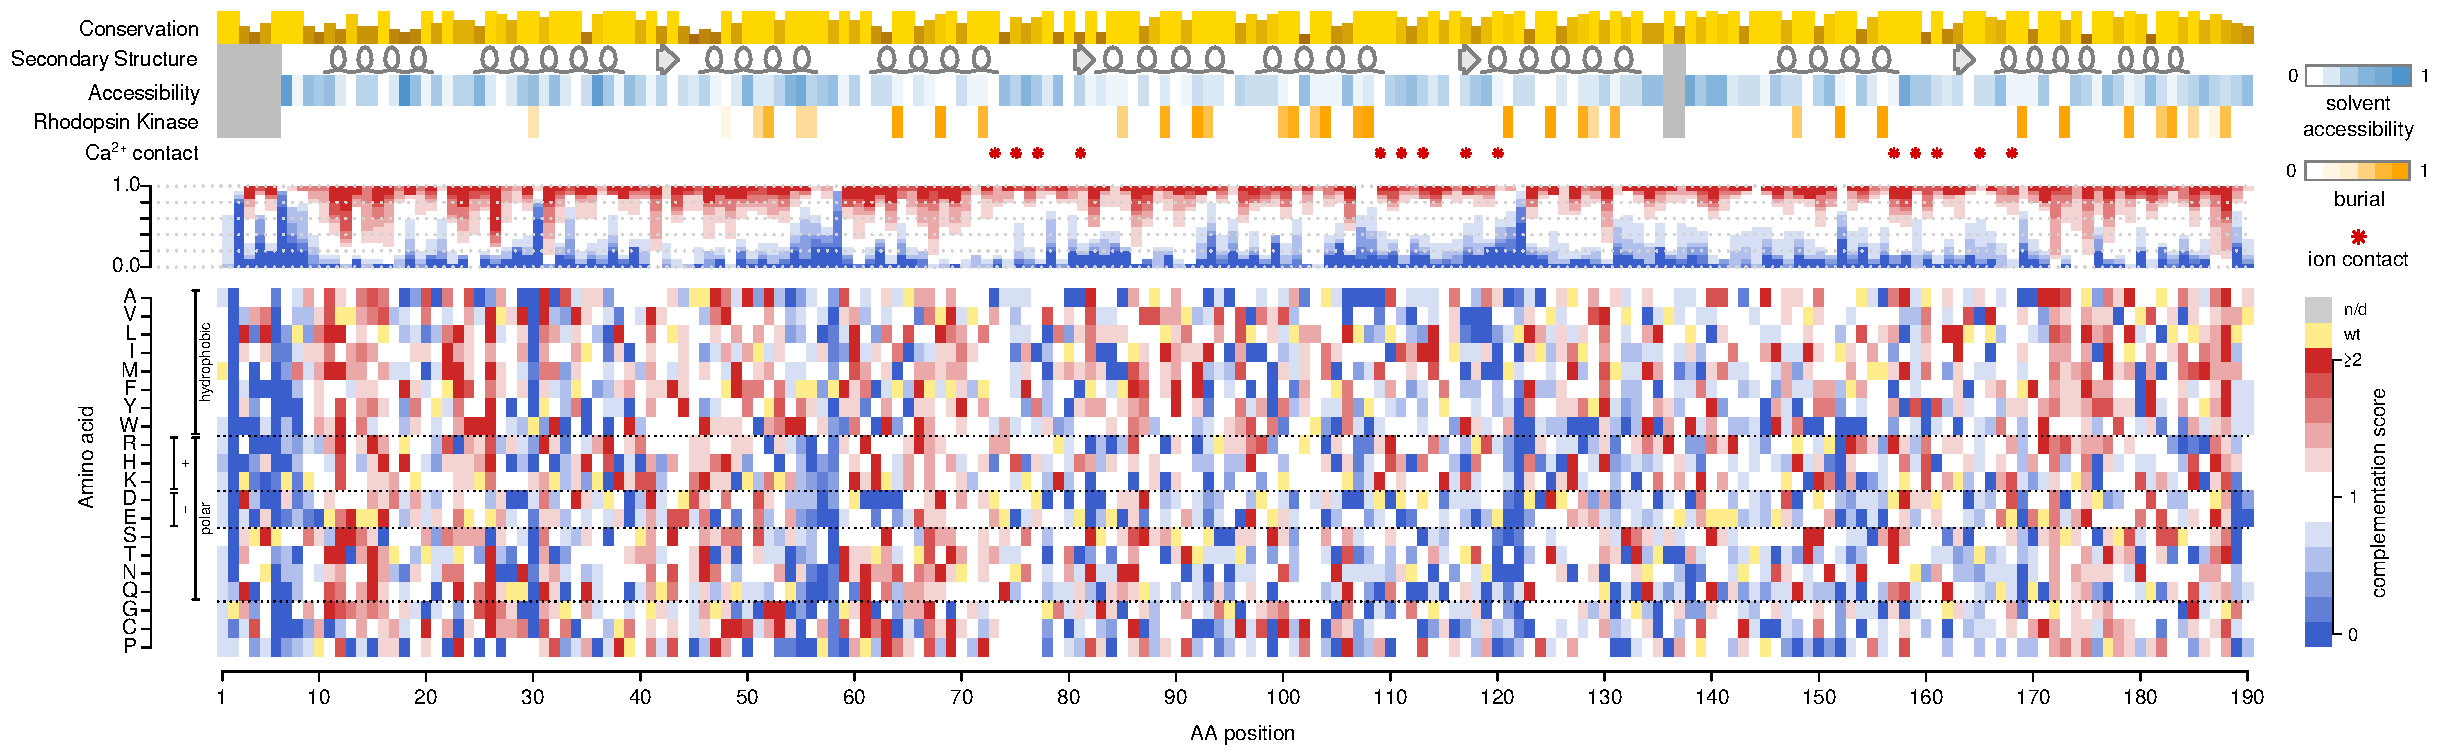
\includegraphics[width=9in]{img/ncs1_map_noflip.pdf}
	\caption{Functional map of NCS1. From top to bottom: Position-wise evolutionary conservation (AMAS); Secondary structure; Relative solvent accessibility; Relative burial in interaction interface with rhodopsin kinase; Positions contacting Calcium ions; A summary track showing the relative number of amino acid changes resulting in different fitness effects; and finally the individual amino acid change effects sorted by physicochemical groups.}
\end{figure}
\end{landscape}


\begin{landscape}
\begin{figure}[h]
	\centering
	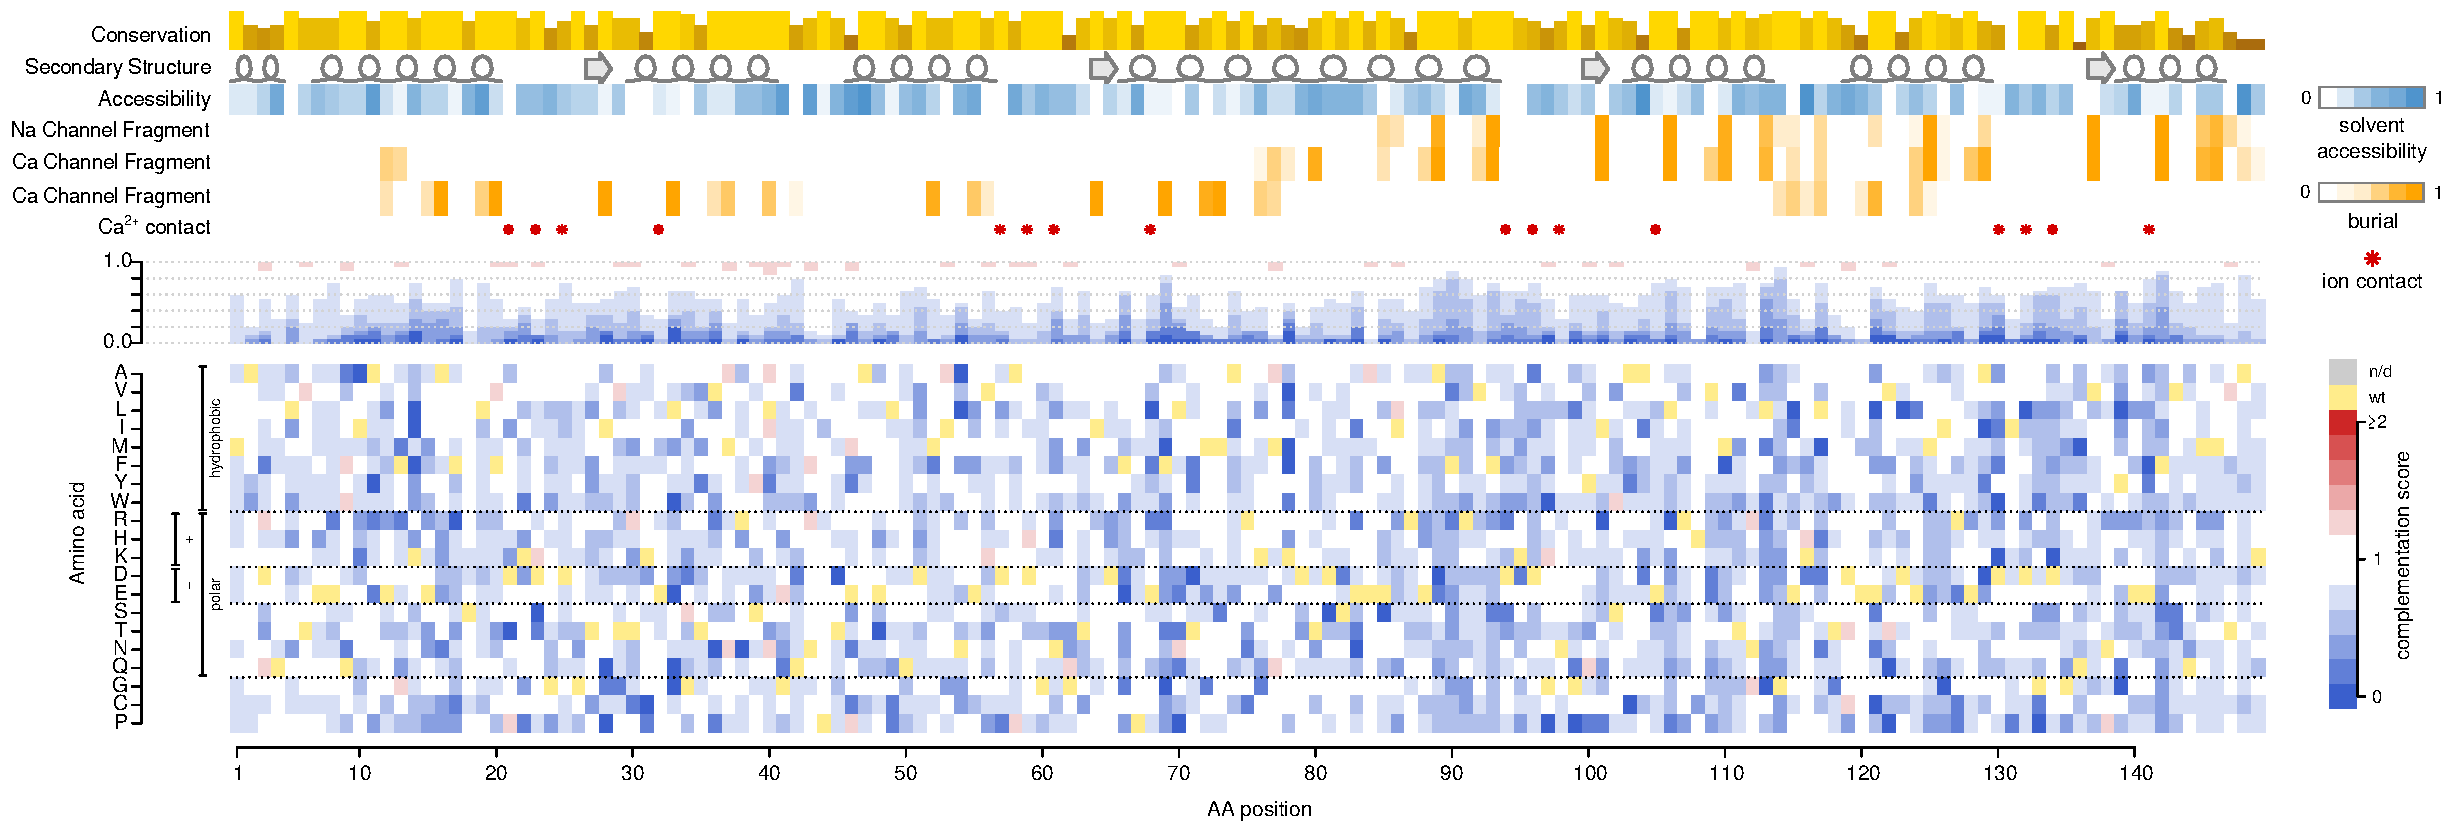
\includegraphics[width=9in]{img/calm1_map_noflip.pdf}
	\caption{Functional map of Calmodulin. From top to bottom: Position-wise evolutionary conservation (AMAS); Secondary structure; Relative solvent accessibility; Relative burial in interaction interface with ion channel fragments; Positions contacting Calcium ions; A summary track showing the relative number of amino acid changes resulting in different fitness effects; and finally the individual amino acid change effects sorted by physicochemical groups.}
\end{figure}
\end{landscape}

\end{appendices}

%% This adds a line for the Bibliography in the Table of Contents.
\addcontentsline{toc}{chapter}{Bibliography}
\bibliographystyle{unsrt}
{\small
\bibliography{thesis_ascii}
}
\end{document}
